\documentclass{beamer}
\usepackage{amsfonts,amsmath,oldgerm,algorithmic,algorithm}
\usepackage{caption} % Required for specifying captions to tables and figures
\usepackage{tikz}
\usetikzlibrary{shapes.callouts, calc}


\usepackage{geometry}
% \usepackage{subfigure, subcaption}
\usepackage{subcaption}
\usepackage[append]{beamersubframe}
% \usepackage{appendixify}
% \usepackage{hyperref}
\hypersetup{%
  colorlinks=false,% hyperlinks will be black
  urlbordercolor = black,
  % linkbordercolor=red,% hyperlink borders will be red
  pdfborderstyle={/S/U/W 1}% border style will be underline of width 1pt
}

\captionsetup{font=tiny,labelfont=bf,skip=-3pt,justification=centering}
\usepackage{booktabs}
\usetheme{CERN}
% \usetheme{Boadilla}

% \beamertemplategridbackground[1cm]
\setbeamersize
{
    text margin left=1cm,
    text margin right=1cm
}

\AtBeginSection[]{
  \begin{frame}
  \vfill
  \centering
  \begin{beamercolorbox}[sep=8pt,center,shadow=false,rounded=false]{title}
    \usebeamerfont{title}\insertsectionhead\par%
  \end{beamercolorbox}
  \vfill
  \end{frame}
}

% Directory for plots
\newcommand{\plots}{./plots}
% \newcommand{\chi2}{\chi^2}
\title{Follow Up DQ Checks of 2024 Data}
\subtitle{Track Variables}
\author{Pawan Johnson}
\institute{University of Liverpool}
\date{\today}


\begin{document}

\begingroup
\setbeamertemplate{footline}{}
\begin{frame}
    \maketitle
\end{frame}
\endgroup

\begin{frame}{Recap on Previous Talk}
    \begin{itemize}
        \small
        \item Main take away from the previous talk are [\href{https://indico.cern.ch/event/1488927/}{Link to talk}]
        \item Most variables showed discrepancies between 2023 and 2024
        \begin{itemize}
            \item Track Positions
            \begin{itemize}
                \item More centrally distributed in 2024 data
                \item Y-Position shifted in accordance with the beam angle
            \end{itemize}
            \item Track Momenta and Charges
            \begin{itemize}
                \item Much higher positively charged high momenta tracks
                \item Difference in background between 2023 and 2024.
            \end{itemize}
            \item Track Parameters showed disagreement
            \begin{itemize}
                \item Lower Track $\chi^2$ in 2024 data.
                \item Could come from higher track momenta in 2024
                \item Other parameters like longTracks were also affected
            \end{itemize}
        \end{itemize}
    \end{itemize}    
\end{frame}


\begin{frame}{Data Specification}
    \begin{itemize}
        \item 2023 data can be found in the directory
        \begin{itemize}
            \item \href{/eos/experiment/faser/phys/2023/p0010}{/eos/experiment/faser/phys/2023/p0010}
        \end{itemize}
        \item 2024 data can be found in the directories
        \begin{itemize}
            \item \href{/eos/experiment/faser/phys/2024/p0011, p0012}{/eos/experiment/faser/phys/2024/p0011, p0012}
            % \item \href{/eos/experiment/faser/phys/2024/p0012}{/eos/experiment/faser/phys/2024/p0012}
        \end{itemize}
        \item The runlist (luminosities) used are from:
        \href{/afs/cern.ch/user/t/torrence/public/faser/runlist/2024/faser runlist 2024 stable.csv}{/afs/cern.ch/user/t/torrence/public/faser/runlist/}
        \item Some runs excluded from above list [in Backup]
        \item BCID cut has been applied to the  2023 data
        \item BCID cut has been partially applied to the 2024 data
        \begin{itemize}
            \item p0012 data has the BCID cut applied
            \item p0011 data does not have the BCID cut applied
        \end{itemize}
    \end{itemize}
    
    {\scriptsize \textbf{Note}: The 2024 data is split into two parts due to possible issues in decoding the LHC Fill Pattern. The data in p0011 has issues with the distanceToCollidingBCID.}
\end{frame}

\begin{subframe}{Runs removed from List}
    \begin{columns}
        \begin{column}{0.5 \linewidth}
            \scriptsize \textbf{Problematic Runs in 2023 RunList}
            \begin{itemize}
                \setlength\itemsep{-0.1em}
                \scriptsize
                \item 11214 - 0 Lumi
            \end{itemize}
            \textbf{High Gain Events}
            \begin{itemize}
                \setlength\itemsep{-0.05em}
                \scriptsize
                \item 10417 
                \item 10419 
                \item 10422 
                \item 10424 
                \item 10426 
                \item 10443 
                \item 10526 
                \item 10538 
                \item 11461 
                \item 11463 
                \item 11471 
                \item 11478 
                \item 11480 
                \item 11486 
                \item 11488 
                \item 11491 
                \item 11504 
                \item 11506 
            \end{itemize}
        \end{column}
        \begin{column}{0.5\linewidth}
            \scriptsize \textbf{Problematic Runs in 2024 RunList}
            \begin{itemize}
                \scriptsize
                \item 16851 - Empty EOS directory
                \item 16852 - Empty EOS directory
                \item Others highlighted in Yield Plots
            \end{itemize}
        \end{column}
    \end{columns}
\end{subframe}


\begin{frame}{Introduction}
    \textbf{Objectives of this Follow up:}
    \begin{itemize}
        \item Module Level Analysis
        \item[] - Look at the DQ checks at the module level
        \item Runwise Analysis for 2024 runs
        \item[] - Look at each run-period in 2024 to identify any issues
        \item Binned Momentum Analysis
        \item[] - Looking at the data binned by momenta 
        \item[] - Should elevate any momenta-based-differences between the years
        \item Reweighed Analysis
        \item[] - Reweighing the 2024 data to match the 2023 momenta
        \item[] - Should make the data more comparable
    \end{itemize}
\end{frame}
% \begin{frame}{Module Level DQ Checks}
%     \begin{itemize}
%         \item Some new variables were introduced in the 2024 data
%         \begin{itemize}
%             \item module\_eta0, module\_phi0
%             \item which describes the first tracking module hit by the particle
%         \end{itemize}
%         \item Idea is to look at the track variables as a function of this
%         \begin{itemize}
%             \item Since, variables not present in 2023 data
%             \item Eta0 and Phi0 are estimated using Track\_x0 and Track\_y0
%         \end{itemize}
%         % \item Unfortunately, 8 modules across 2 year = 16 Histograms 
%         % \begin{itemize}
%         %     \item Hard to visualize, so we do a module level comparison
%         %     \item More detailed plots available in the backup/repo
%         % \end{itemize}
        

%     \end{itemize}
% \end{frame}

\begin{frame}{Module Numbering Schematic }
    \begin{figure}
        \hspace{-1cm}
        \begin{tikzpicture}[scale=0.24]
            % \draw[step=1cm,gray!30,very thin] (-12,-12) grid (12,12);

            \draw[-,thick] (0,-12) -- (0,12);
            \draw[-,thick] (-12,-12) -- (-12,12);
            \draw[-,thick] (12,-12) -- (12,12);


            \draw[-, thick] (-12, -12) -- (12, -12);
            \draw[-, thick] (-12, -6) -- (12, -6);
            \draw[-, thick] (-12, 0) -- (12, 0);
            \draw[-, thick] (-12, 6) -- (12, 6);
            \draw[-, thick] (-12, 12) -- (12, 12);

            \node[rectangle, draw=none, minimum size=1pt] at ( -6 , 9 )  {Module 1};
            \node[rectangle, draw=none, minimum size=1pt] at ( -6 , 3 )  {Module 2};
            \node[rectangle, draw=none, minimum size=1pt] at ( -6 , -3 ) {Module 3};
            \node[rectangle, draw=none, minimum size=1pt] at ( -6 , -9 ) {Module 4};

            \node[rectangle, draw=none, minimum size=1pt] at ( 6 , -9 )  {Module 5};
            \node[rectangle, draw=none, minimum size=1pt] at ( 6 , -3 )  {Module 6};
            \node[rectangle, draw=none, minimum size=1pt] at ( 6 , 3 )   {Module 7};
            \node[rectangle, draw=none, minimum size=1pt] at ( 6 , 9 )   {Module 8};

            \draw[->, thick] (-13, -13) -- (-13, 13.5) node[above right] {$y$};
            \draw[->, thick] (-13, -13) -- (13, -13) node[right] {$x$};
            
            \draw[- , thick] (-13, -12) -- (-12.5, -12) node[left=0.1cm] {-120}; 
            \draw[- , thick] (-13,  -6) -- (-12.5,  -6) node[left=0.1cm] {-60}; 
            \draw[- , thick] (-13,   0) -- (-12.5,   0) node[left=0.1cm] {0}; 
            \draw[- , thick] (-13,   6) -- (-12.5,   6) node[left=0.1cm] {60}; 
            \draw[- , thick] (-13,  12) -- (-12.5,  12) node[left=0.1cm] {120}; 

            \draw[- , thick] (-12, -13) -- (-12, -12.5) node[below=0.1cm] {-120};
            \draw[- , thick] (0,   -13) -- (0,   -12.5) node[below=0.1cm] {0}; 
            \draw[- , thick] (12,  -13) -- (12,  -12.5) node[below=0.1cm] {12}; 

            \node at (-17, -9) {Phi = 0};
            \node at (-17, -3) {Phi = 1};
            \node at (-17, +3) {Phi = 2};
            \node at (-17, +9) {Phi = 3};

            \node at (-6, -14.7) {Eta = -1};
            \node at (+6, -14.7) {Eta = +1};

            % \node[rectangle, draw=none, minimum size=1pt] at ( -6 , 9 )  {Module 1};
        \end{tikzpicture}
        \caption{Module Boundaries Schematic. Numbering borrowed from Angela's Schematic}
    \end{figure}
\end{frame}

% \begin{frame}{Module Level Splitting}
%     \begin{columns}
%         \begin{column}{1.2\linewidth}
%             \begin{figure}
%                 \centering
%                 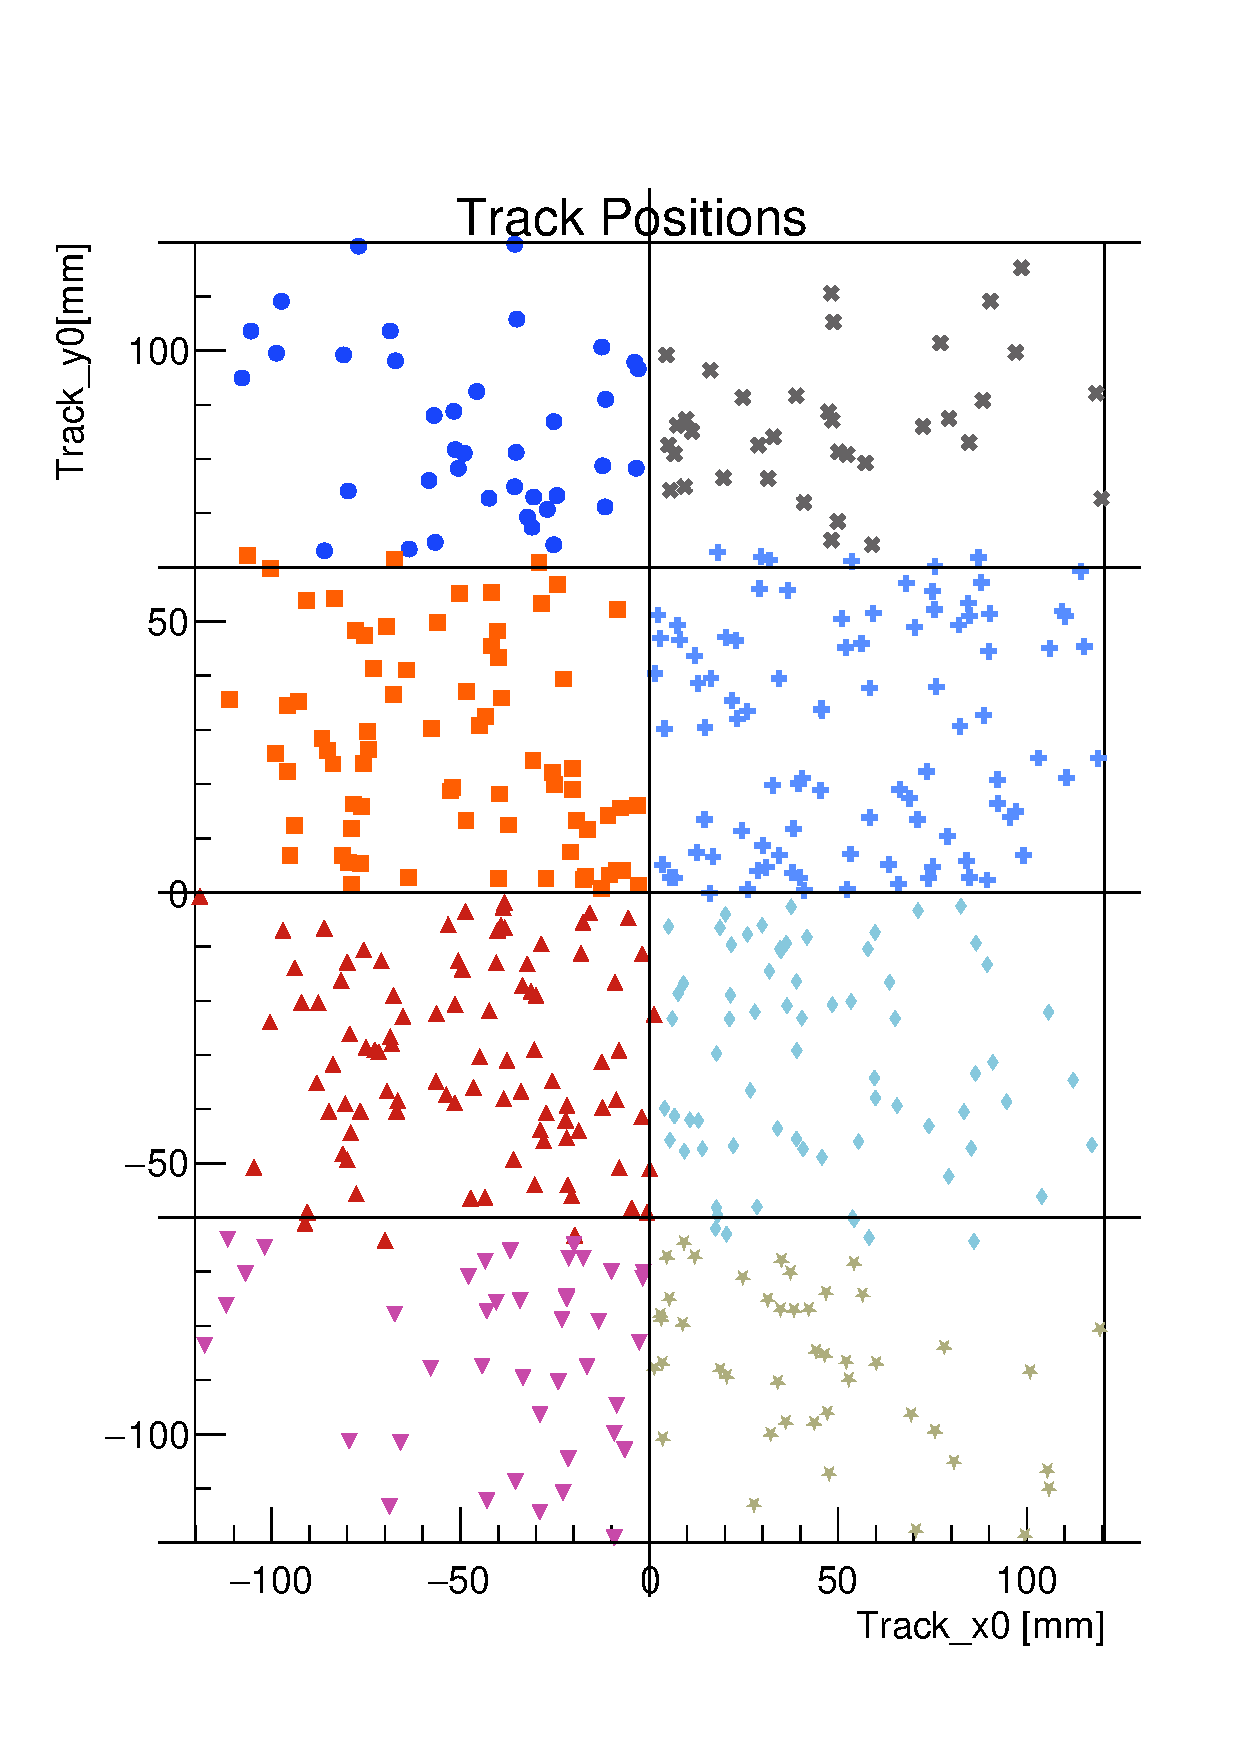
\includegraphics[height=0.8\textheight]{./ModuleLevelPlots/Positions_st0_truemodule0.pdf}
%                 \caption{500 Points at Station-1 colored according to module-variables in 2024 data}
%             \end{figure}
%         \end{column}
%         \begin{column}{0.2\linewidth}
%             \begin{figure}
%                 \hspace{-7cm}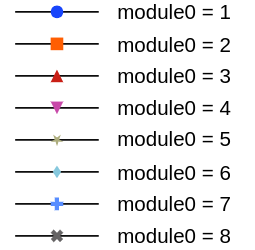
\includegraphics[scale=0.25]{./assets/image.png}
%             \end{figure}
%         \end{column}
%     \end{columns}
% \end{frame}

% \begin{frame}{Where are the Module Boundaries?}
%     \begin{columns}
%         \begin{column}{0.5 \linewidth}
%             \begin{figure}
%                 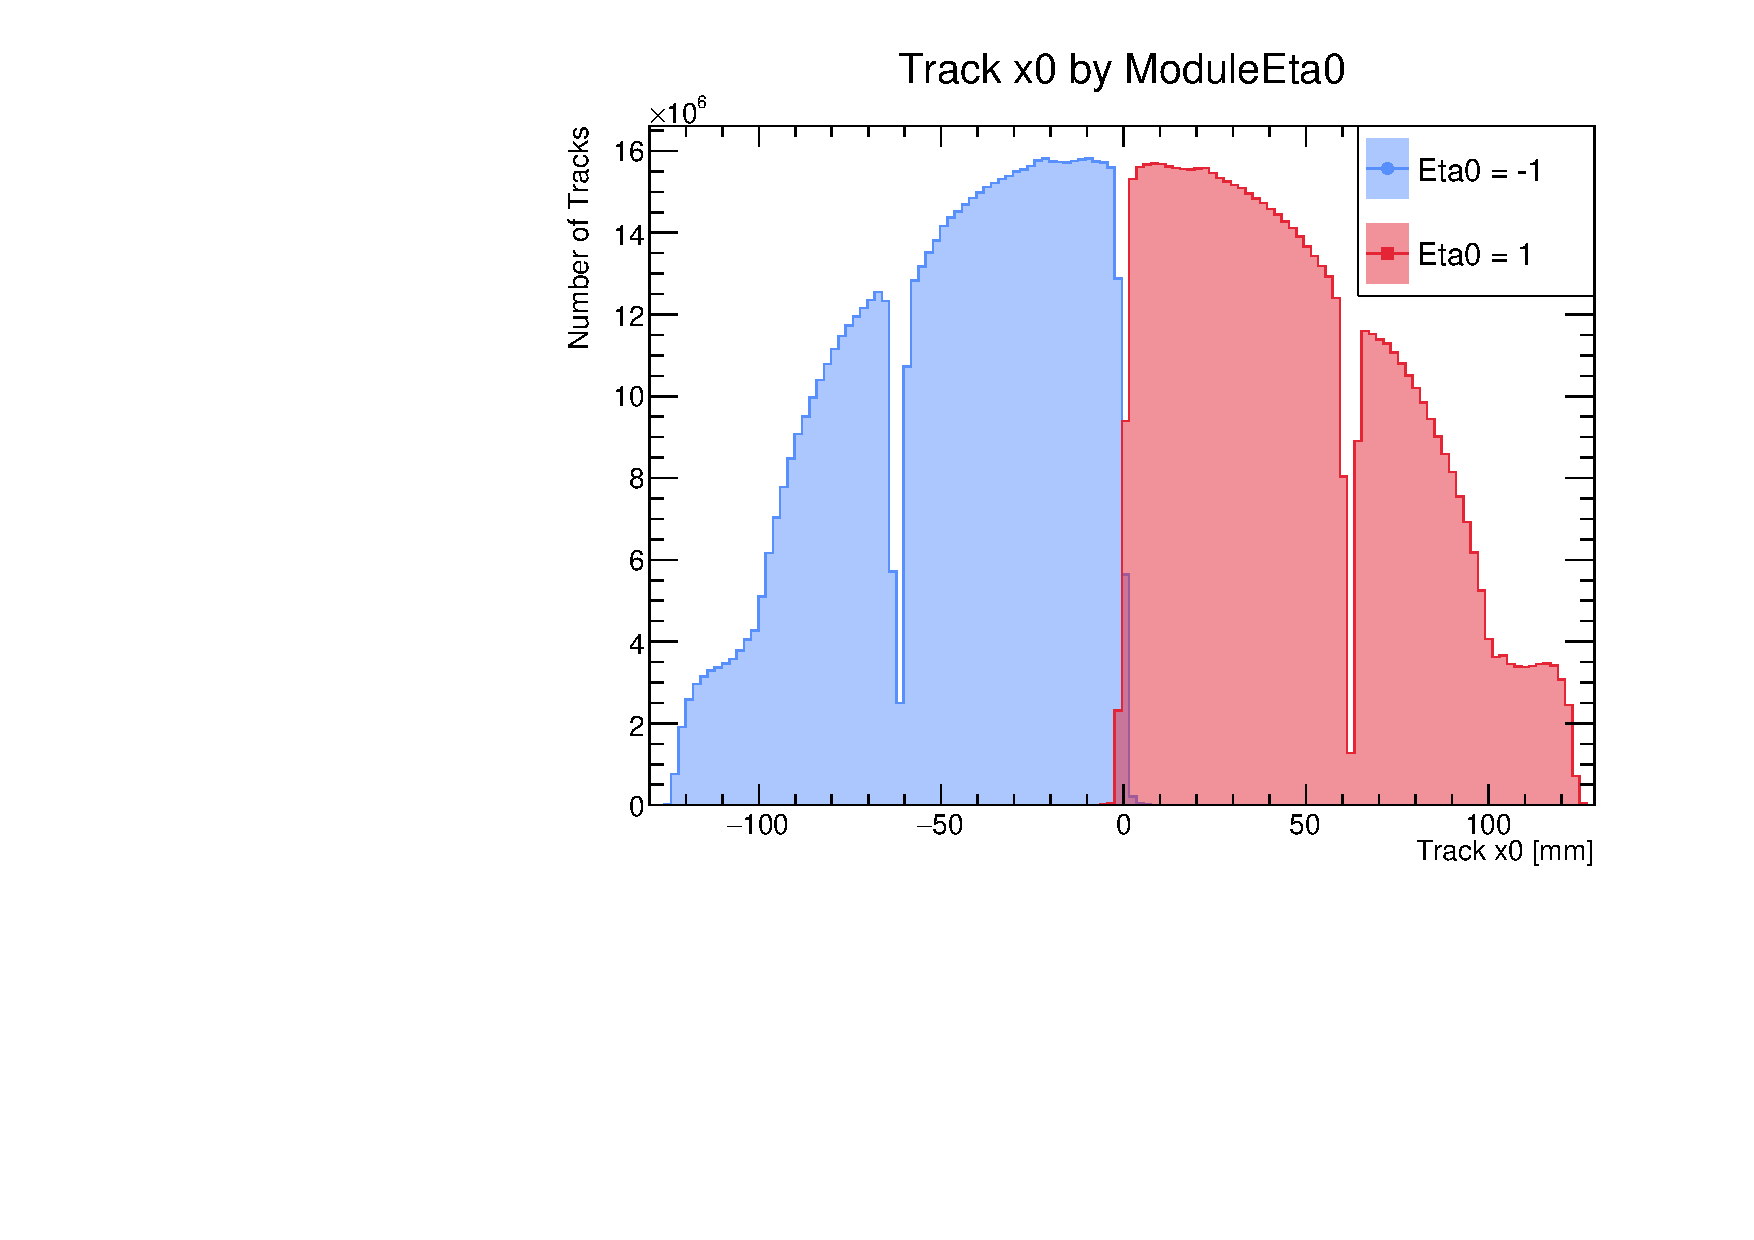
\includegraphics[width=\linewidth]{./ModuleLevelPlots/Track_x0_eta0.pdf}
%                 \caption{Track Positions at Station 1 colored by module\_eta0}
%             \end{figure}
%         \end{column}
%         \begin{column}{0.5 \linewidth}
%             \begin{figure}
%                 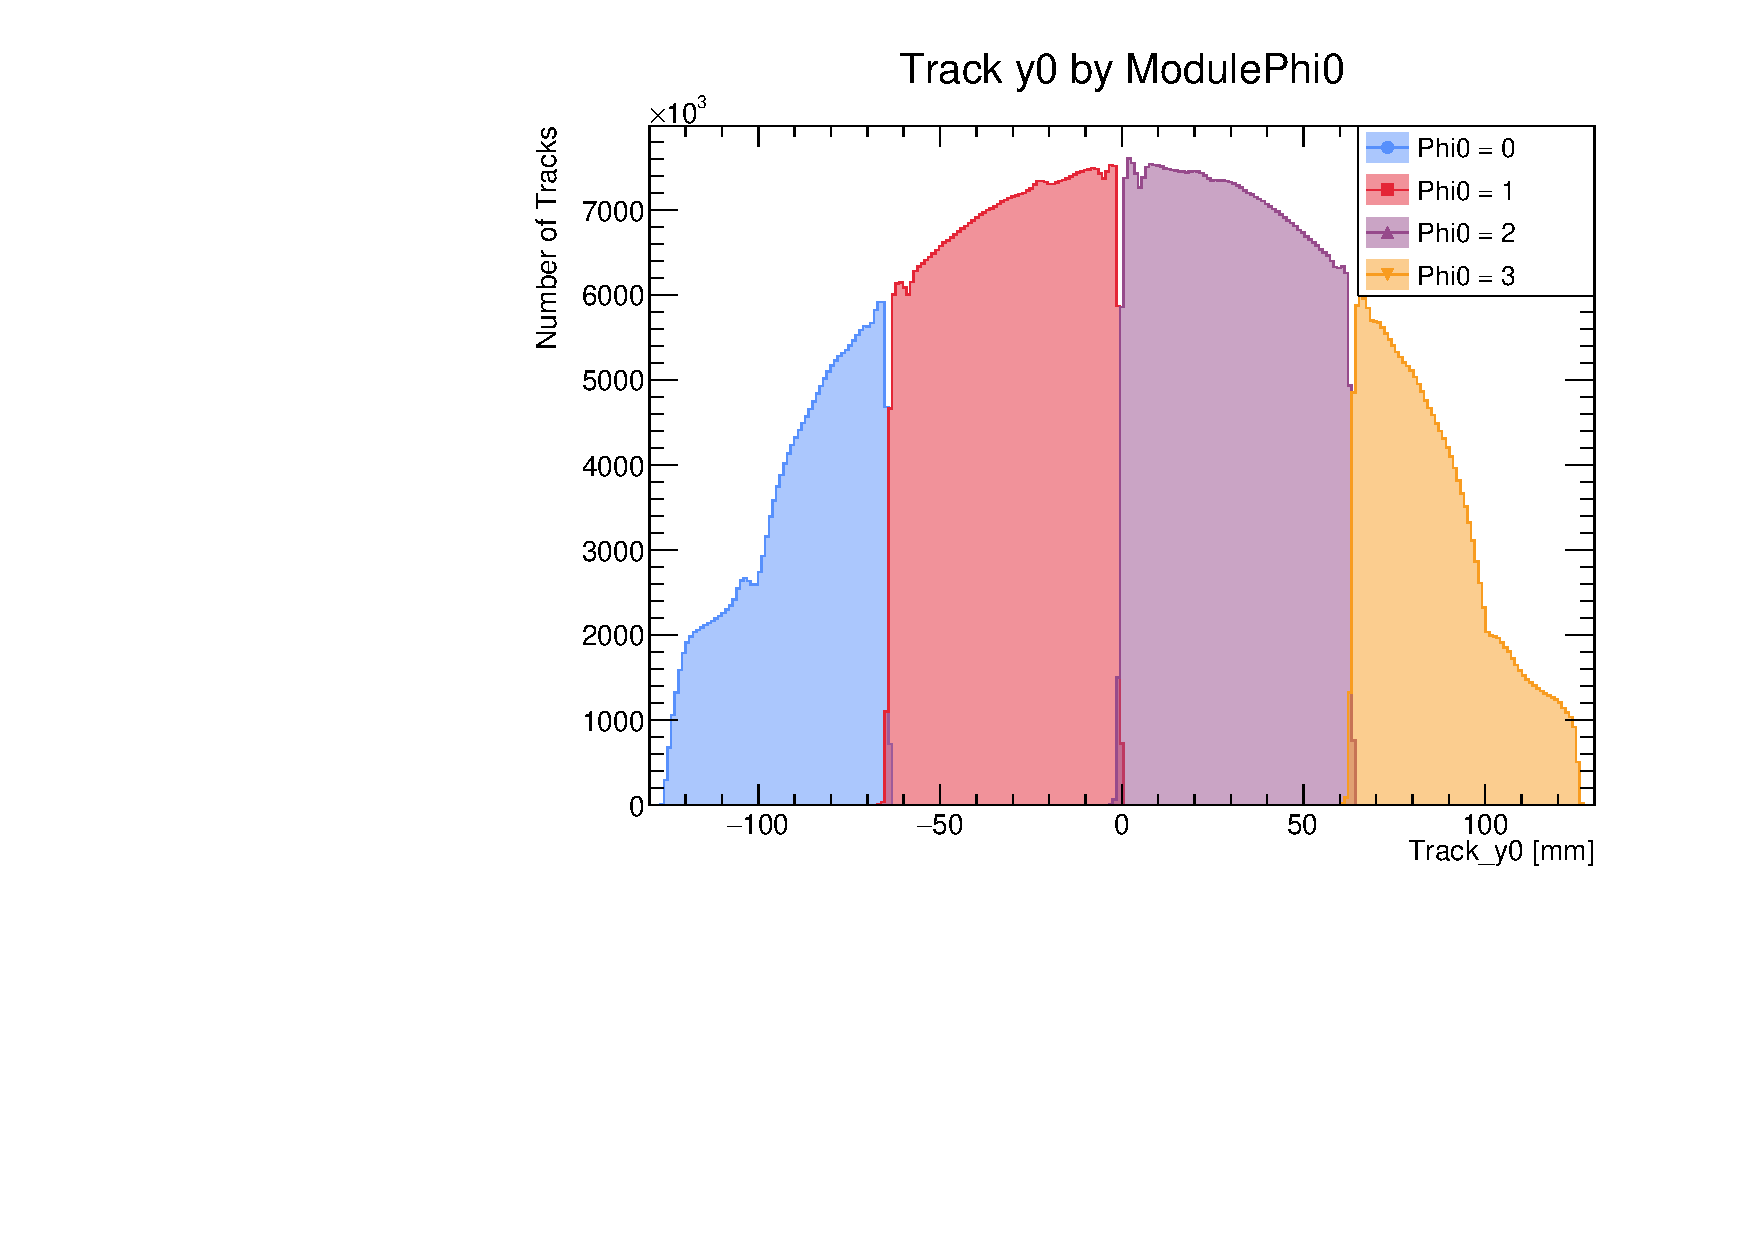
\includegraphics[width=\linewidth]{./ModuleLevelPlots/Track_y0_phi0.pdf}
%                 \caption{Track Positions at Station 1 colored by module\_phi0}
%             \end{figure}
%         \end{column}
%      \end{columns}
% \end{frame}




% \begin{frame}{Accuracy of Module Splits}
%     \begin{itemize}
%         \item Since 2023 does not have the module\_eta0 / phi0 entries we approximate them using the above schematic.
%     \end{itemize}
%     \begin{figure}
%         \centering
%         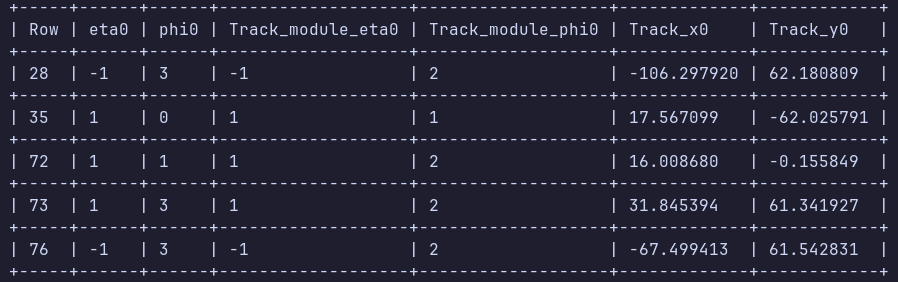
\includegraphics[width=1.0\linewidth]{./assets/ModuleMismatch.png}
%         \caption{Module Calculation mismatch in run 016635}
%     \end{figure}   
%     \begin{itemize}
%         \item Mismatch are within $\pm$ 5 mm of the borders
%         \item Number of Mismatches:  587982  out of  13601766 i.e 4.3\%
%     \end{itemize}
% \end{frame}

% \begin{frame}{Revisiting Positions at Station 1}
%     \begin{columns}
%         \begin{column}{1.2\linewidth}
%             \begin{figure}
%                 \centering
%                 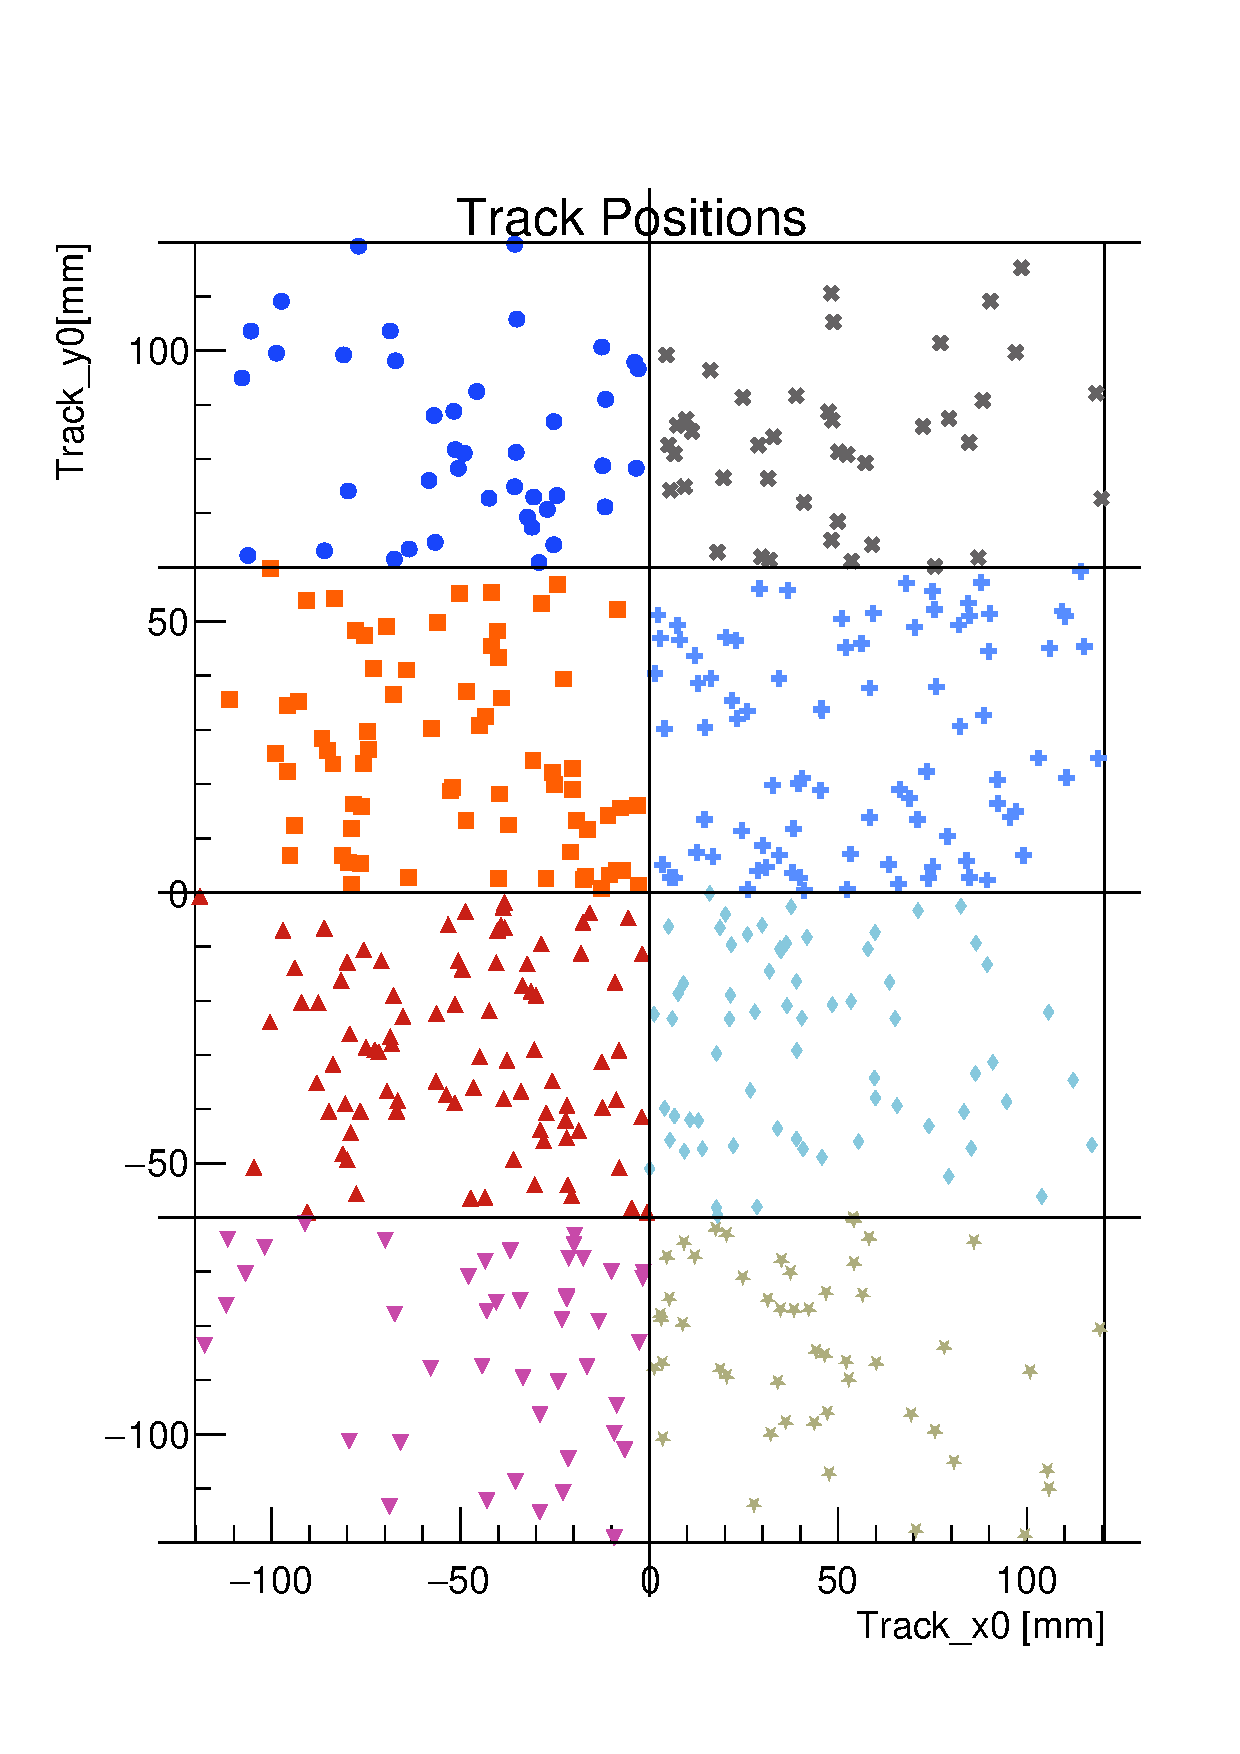
\includegraphics[height=0.8\textheight]{./ModuleLevelPlots/Positions_st0_module0.pdf}
%                 \caption{500 Points at Station 1 colored by Module number (estimated) at Station 1 for 2024 data}
%             \end{figure}
%         \end{column}
%         \begin{column}{0.2\linewidth}
%             \begin{figure}
%                 \hspace{-7cm}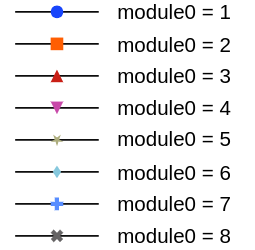
\includegraphics[scale=0.25]{./assets/image.png}
%             \end{figure}
%         \end{column}
%     \end{columns}
% \end{frame}

% \begin{frame}{Where do they end up in Station 3?}
%     \begin{columns}
%         \begin{column}{1.2\linewidth}
%             \begin{figure}
%                 \centering
%                 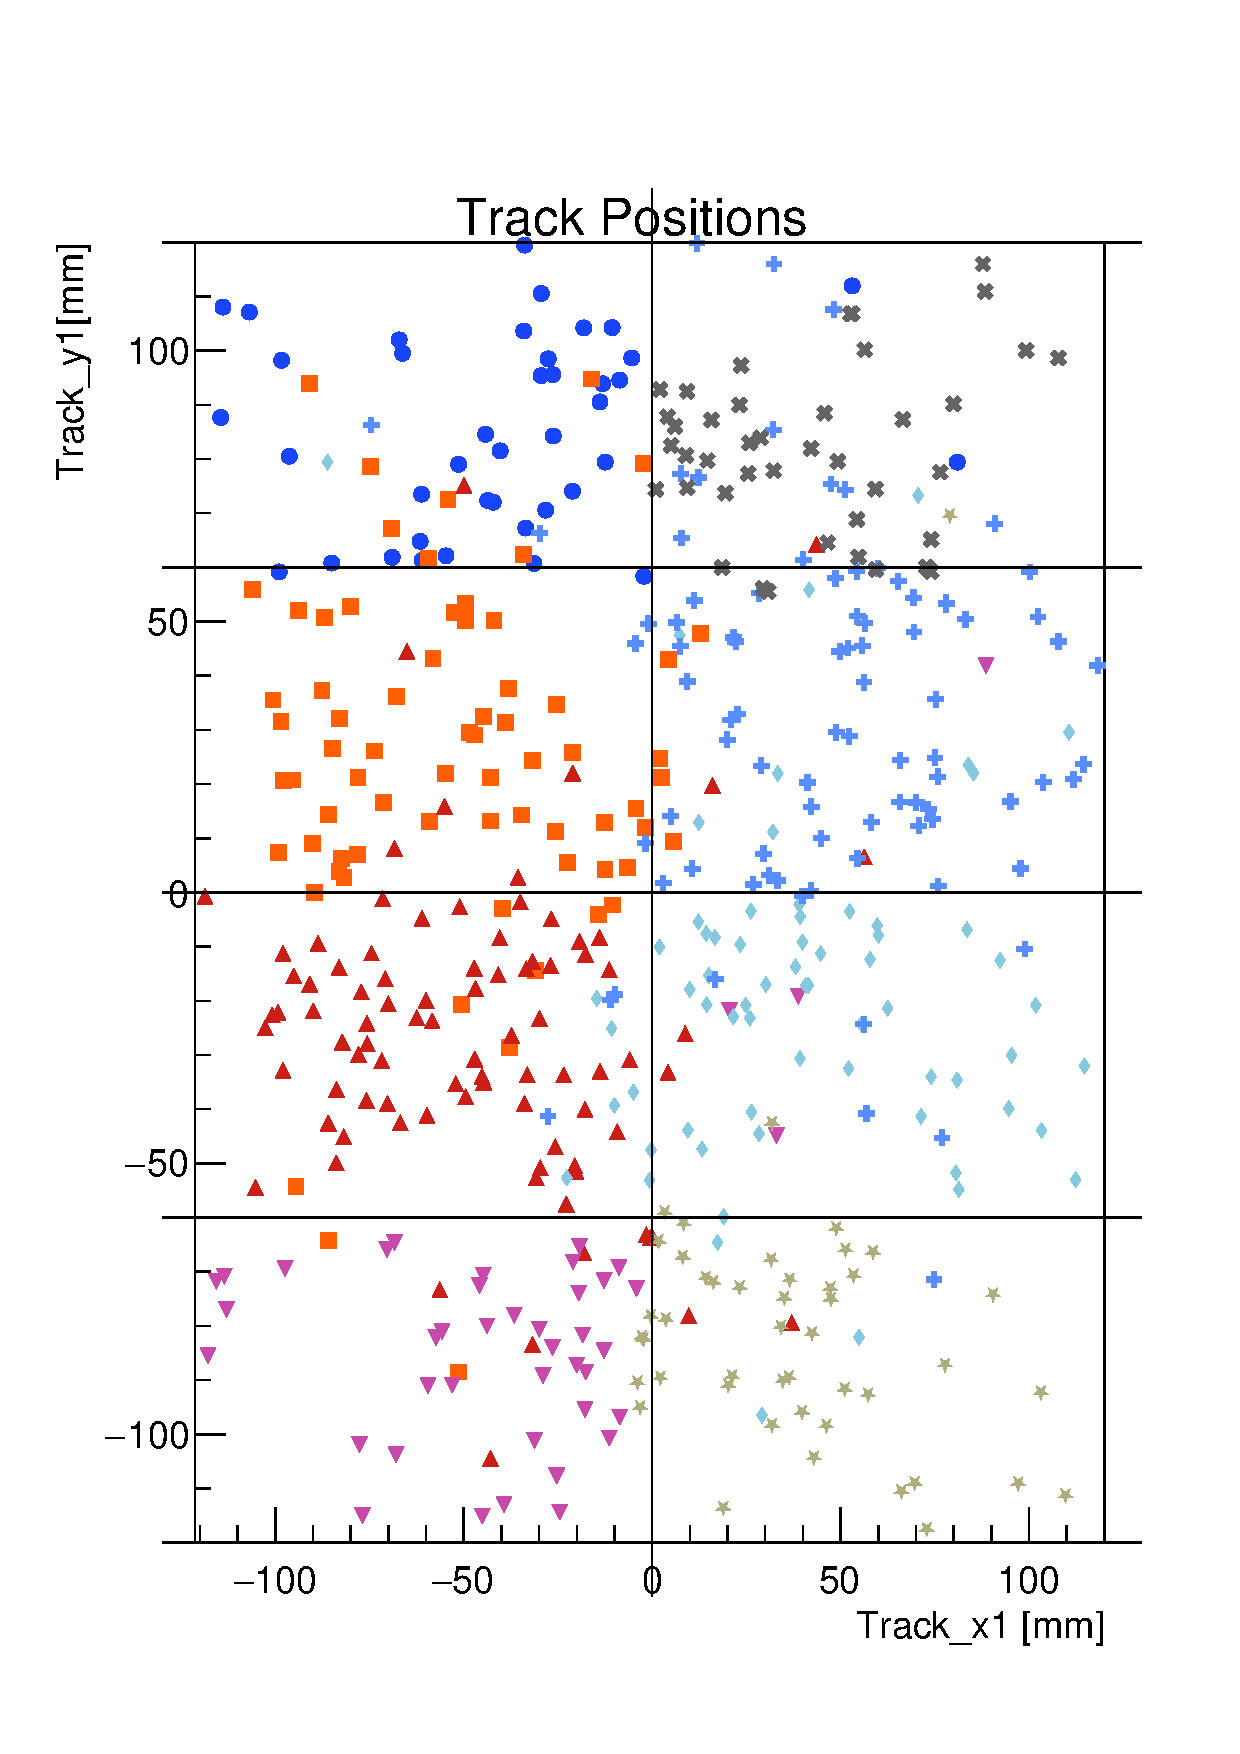
\includegraphics[height=0.8\textheight]{./ModuleLevelPlots/Positions_st1_module0.pdf}
%                 \caption{500 Points at Station 3 colored by Module number at Station 1 for 2024 data [Same tracks as previous slide]}
%             \end{figure}
%         \end{column}
%         \begin{column}{0.2\linewidth}
%             \begin{figure}
%                 \hspace{-7cm}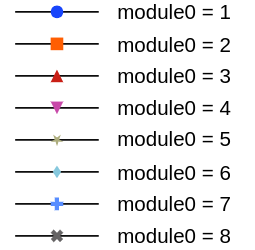
\includegraphics[scale=0.25]{./assets/image.png}
%             \end{figure}
%         \end{column}
%     \end{columns}
% \end{frame}

% \begin{subframe}{Transfer Heatmap in 2023}
%     \begin{columns}
%         \begin{column}{0.85\linewidth}
%             \begin{figure}
%                 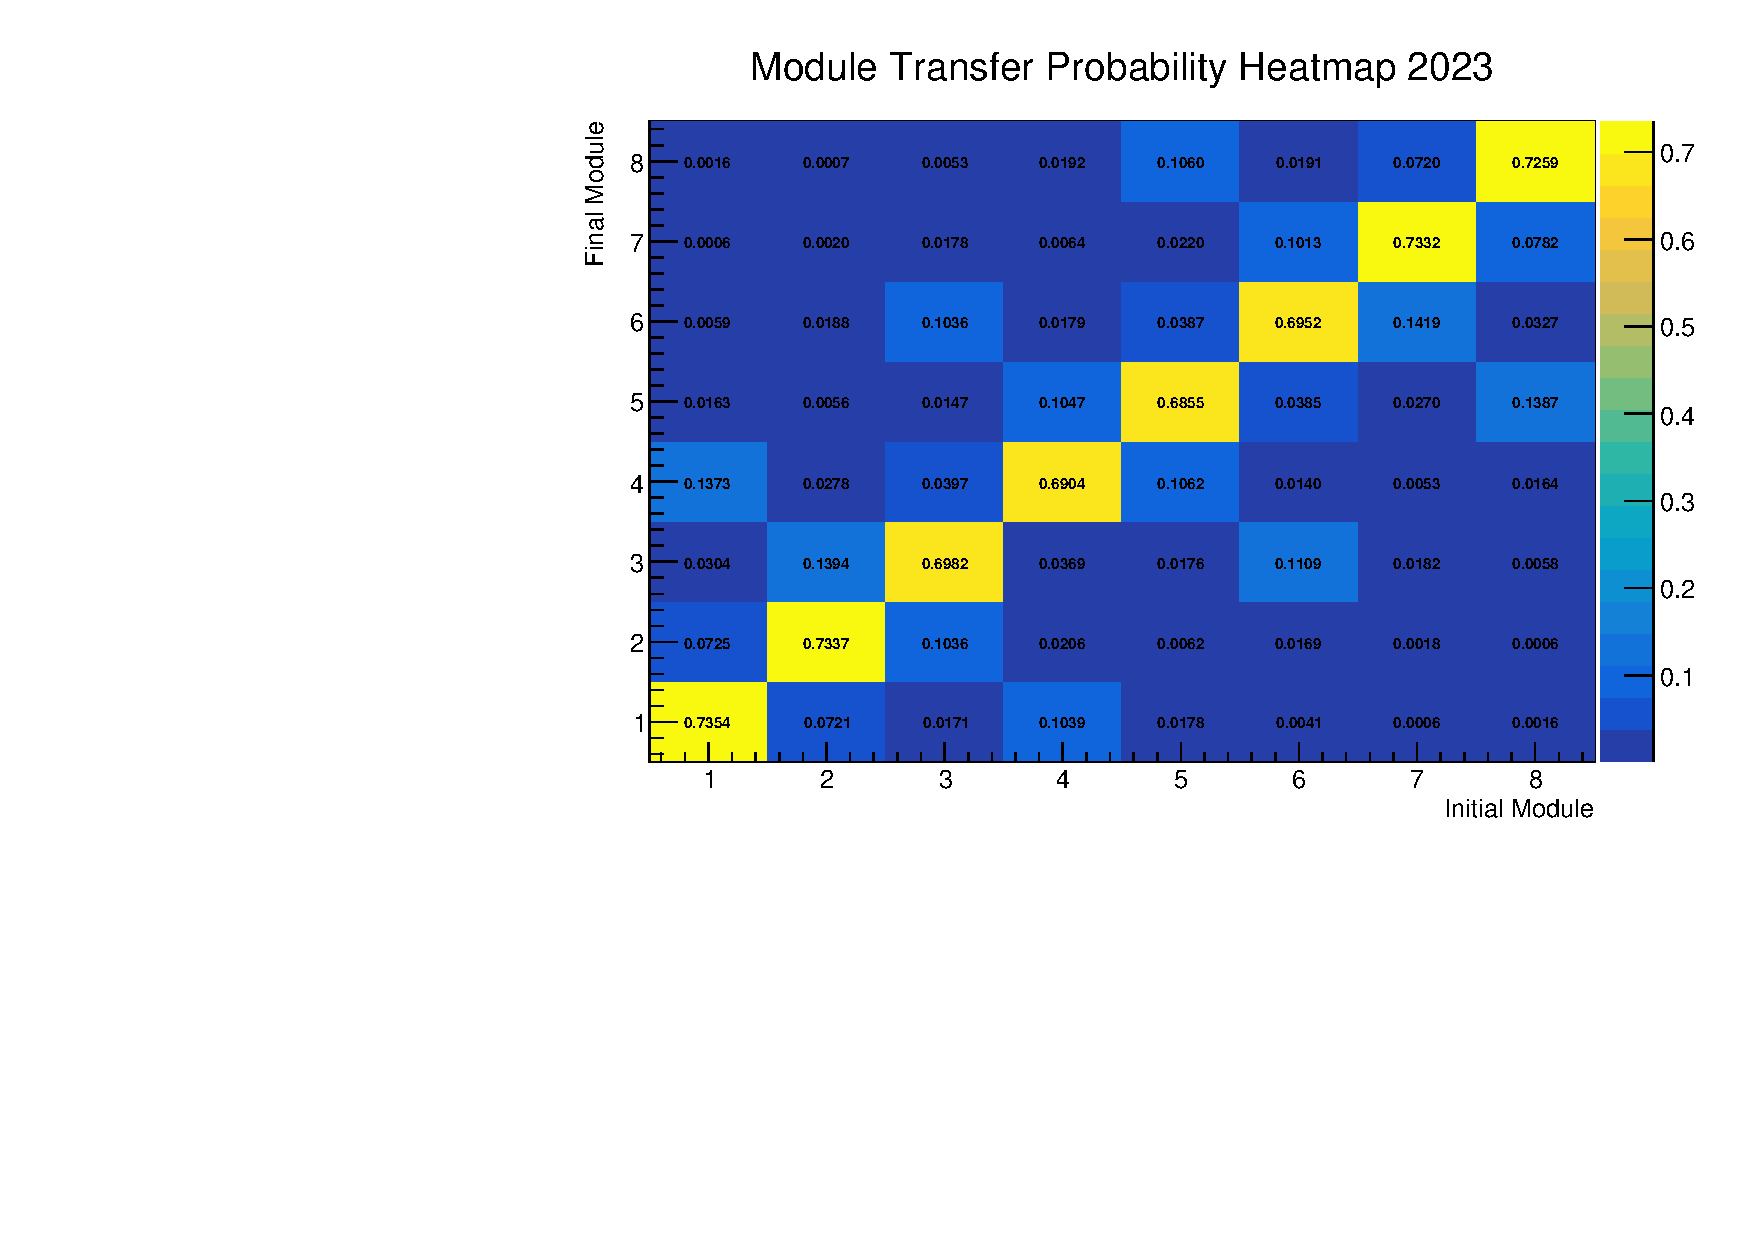
\includegraphics[width=0.9\linewidth]{./ModuleLevelPlots/st0_module_number vs st1_module_number_prob_2023.pdf}
%                 \caption{Probability of Transfer from Initial Module (at Station 1) to Final Module (at Station 2) based on 2023 Data}
%             \end{figure}
%         \end{column}
%         \begin{column}{0.2\linewidth}
%             \begin{figure}
%                 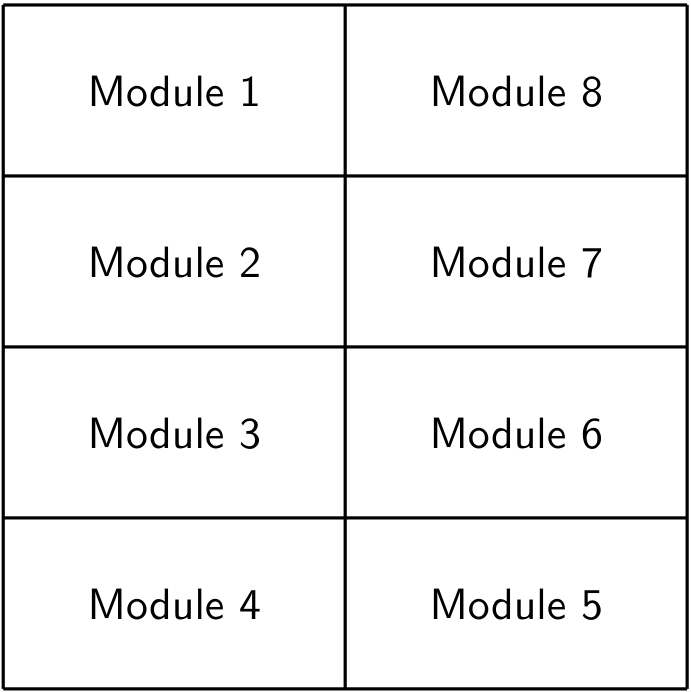
\includegraphics[width=\linewidth]{./assets/ModuleThumbnail.png}
%             \end{figure}
%         \end{column}
%     \end{columns}
%     \begin{itemize}
%         \small
%         \item Most probable transfer is to the same module followed by adjacent.
%         \item Module 2,3,6,7 (central) are more likely to transfer to another central module. 
%     \end{itemize}
% \end{subframe}

% \begin{subframe}{Transfer Heatmap in 2024}
%     \begin{figure}
%         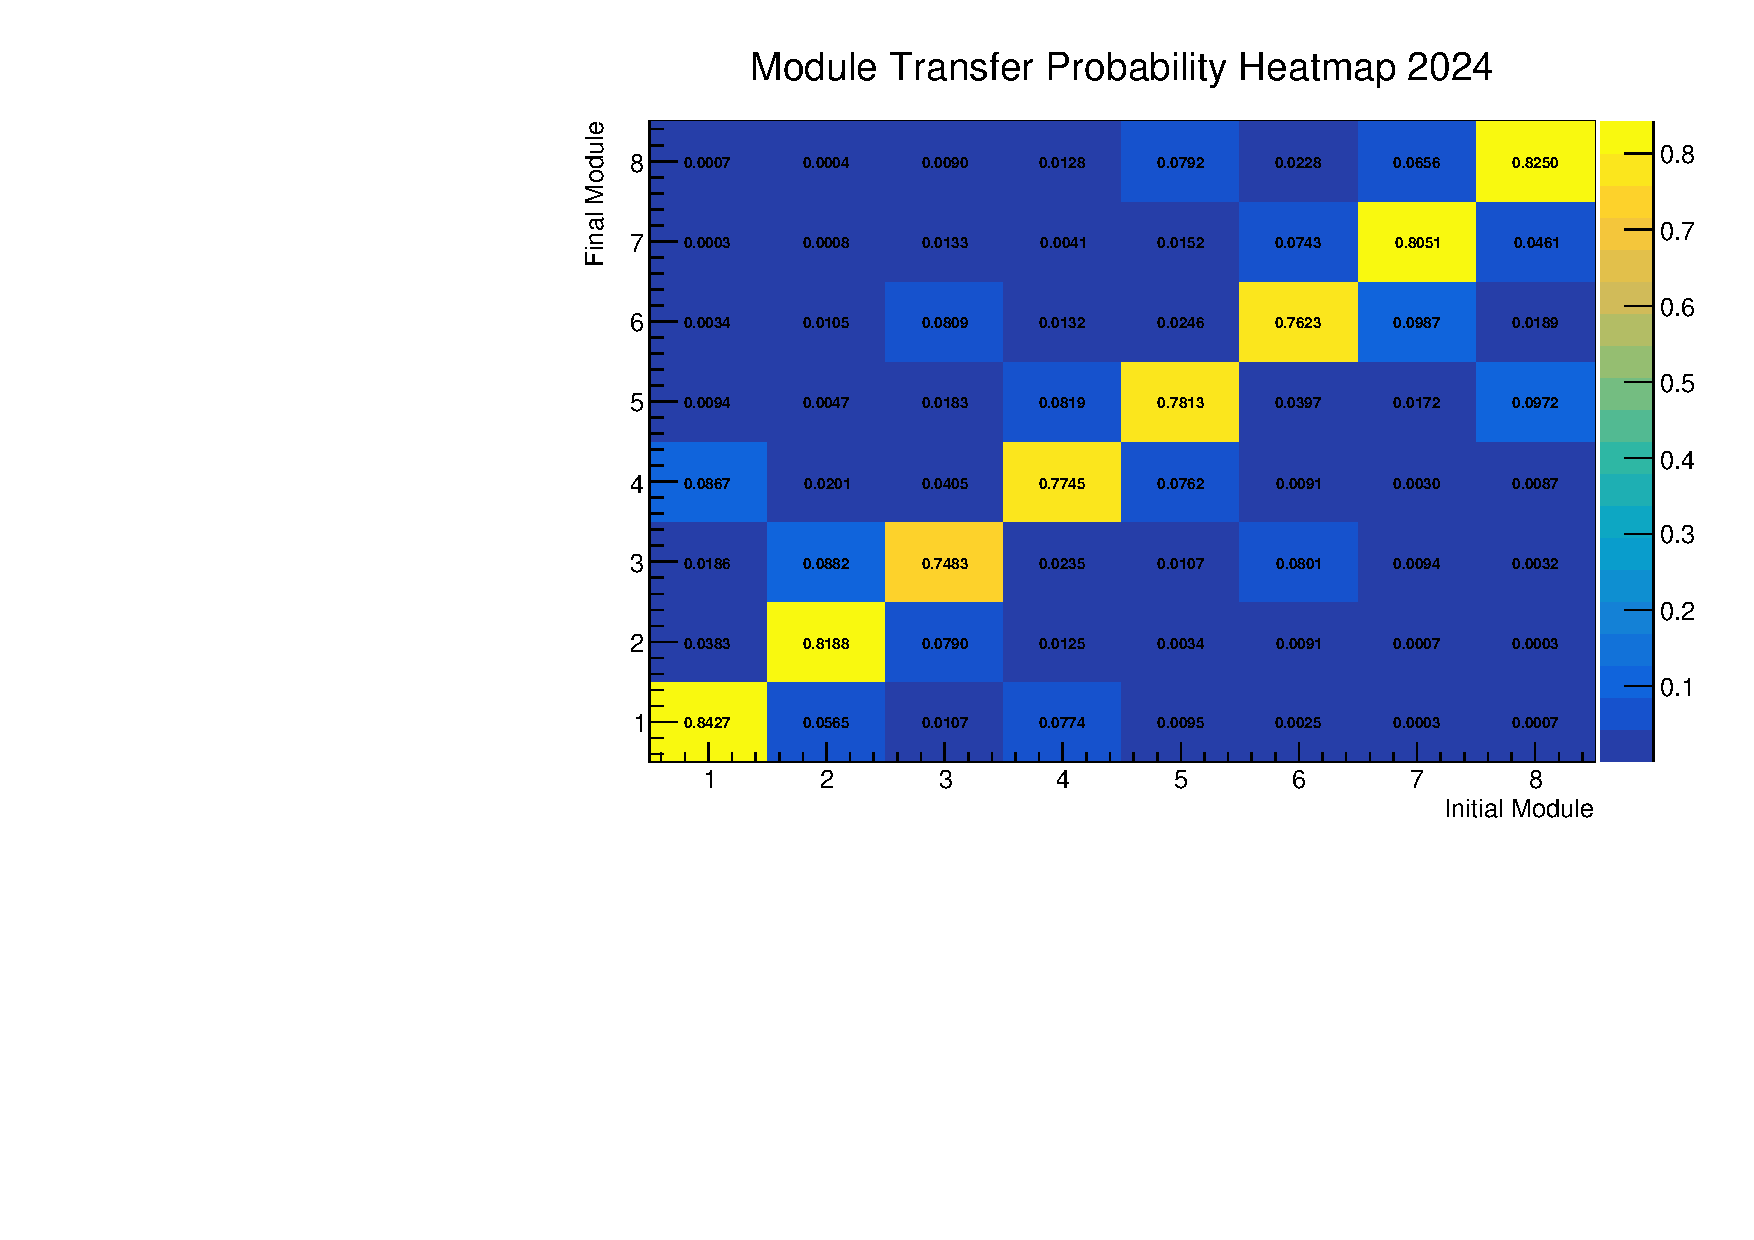
\includegraphics[width=0.8\linewidth]{./ModuleLevelPlots/st0_module_number vs st1_module_number_prob_2024.pdf}
%         \caption{Probability of Transfer from Initial Module (at Station 1) to Final Module (at Station 2) based on 2024 data}
%     \end{figure}
%     \begin{itemize}
%         \small
%         \item Much higher Probability of Transfer to the same module
%         \item In general less module transfers in 2024. [Higher Momentum Tracks]
%     \end{itemize}
% \end{subframe}

% \begin{subframe}{Transfer Heatmap Ratio }
%     \begin{figure}
%         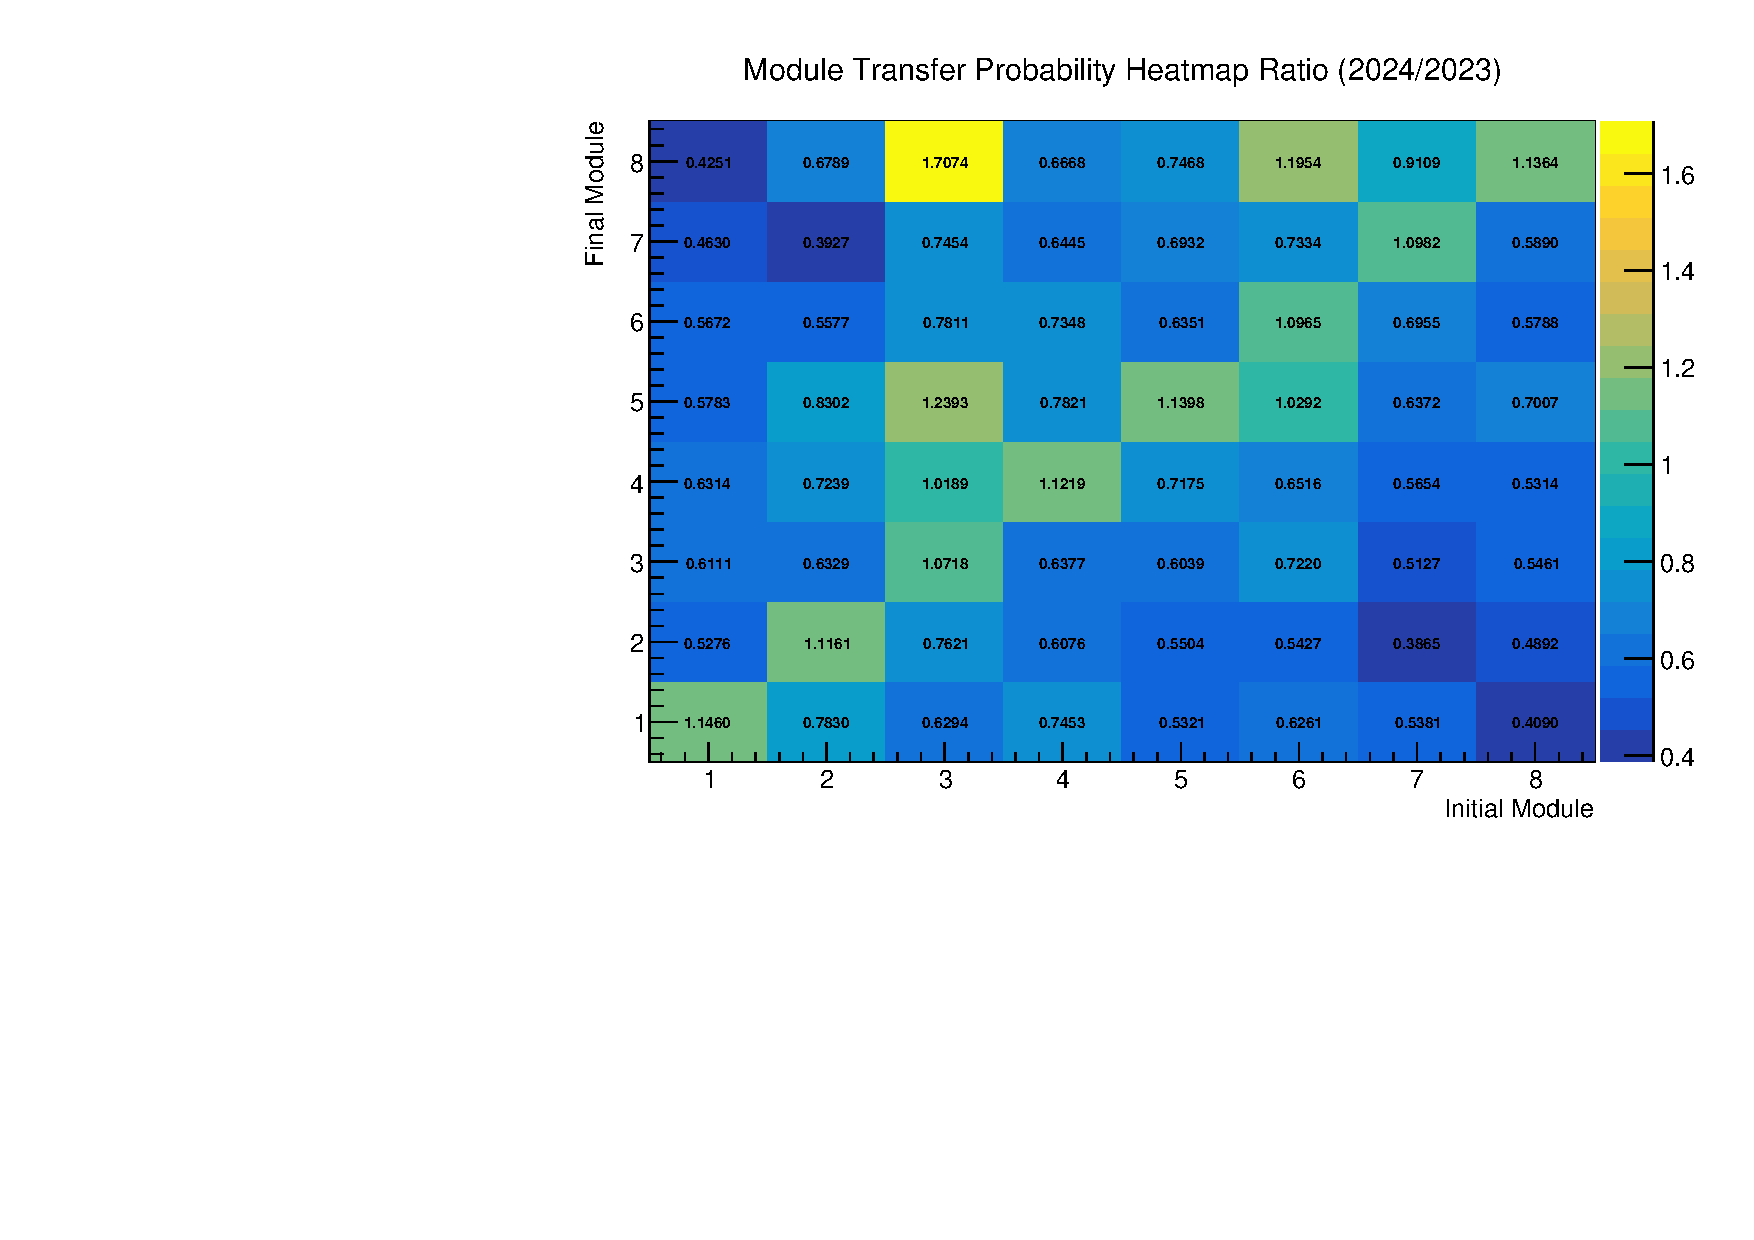
\includegraphics[width=0.86\linewidth]{./ModuleLevelPlots/st0_module_number vs st1_module_number_prob_ratio.pdf}
%         \caption{Ratio of Probability of Transfer from Initial Module (at Station 1) to Final Module (at Station 2) }
%     \end{figure}
%     \begin{itemize}
%         \small
%         \item 2024 has a higher probability of transfer to the same module
%         \item Module 3 and 6 seem to be transferring into 8 more [Why?]
%     \end{itemize}
% \end{subframe}

% \begin{frame}{Transfer Histograms}
%     \begin{figure}
%         \centering
%         \begin{subfigure}[t]{0.49\linewidth}
%             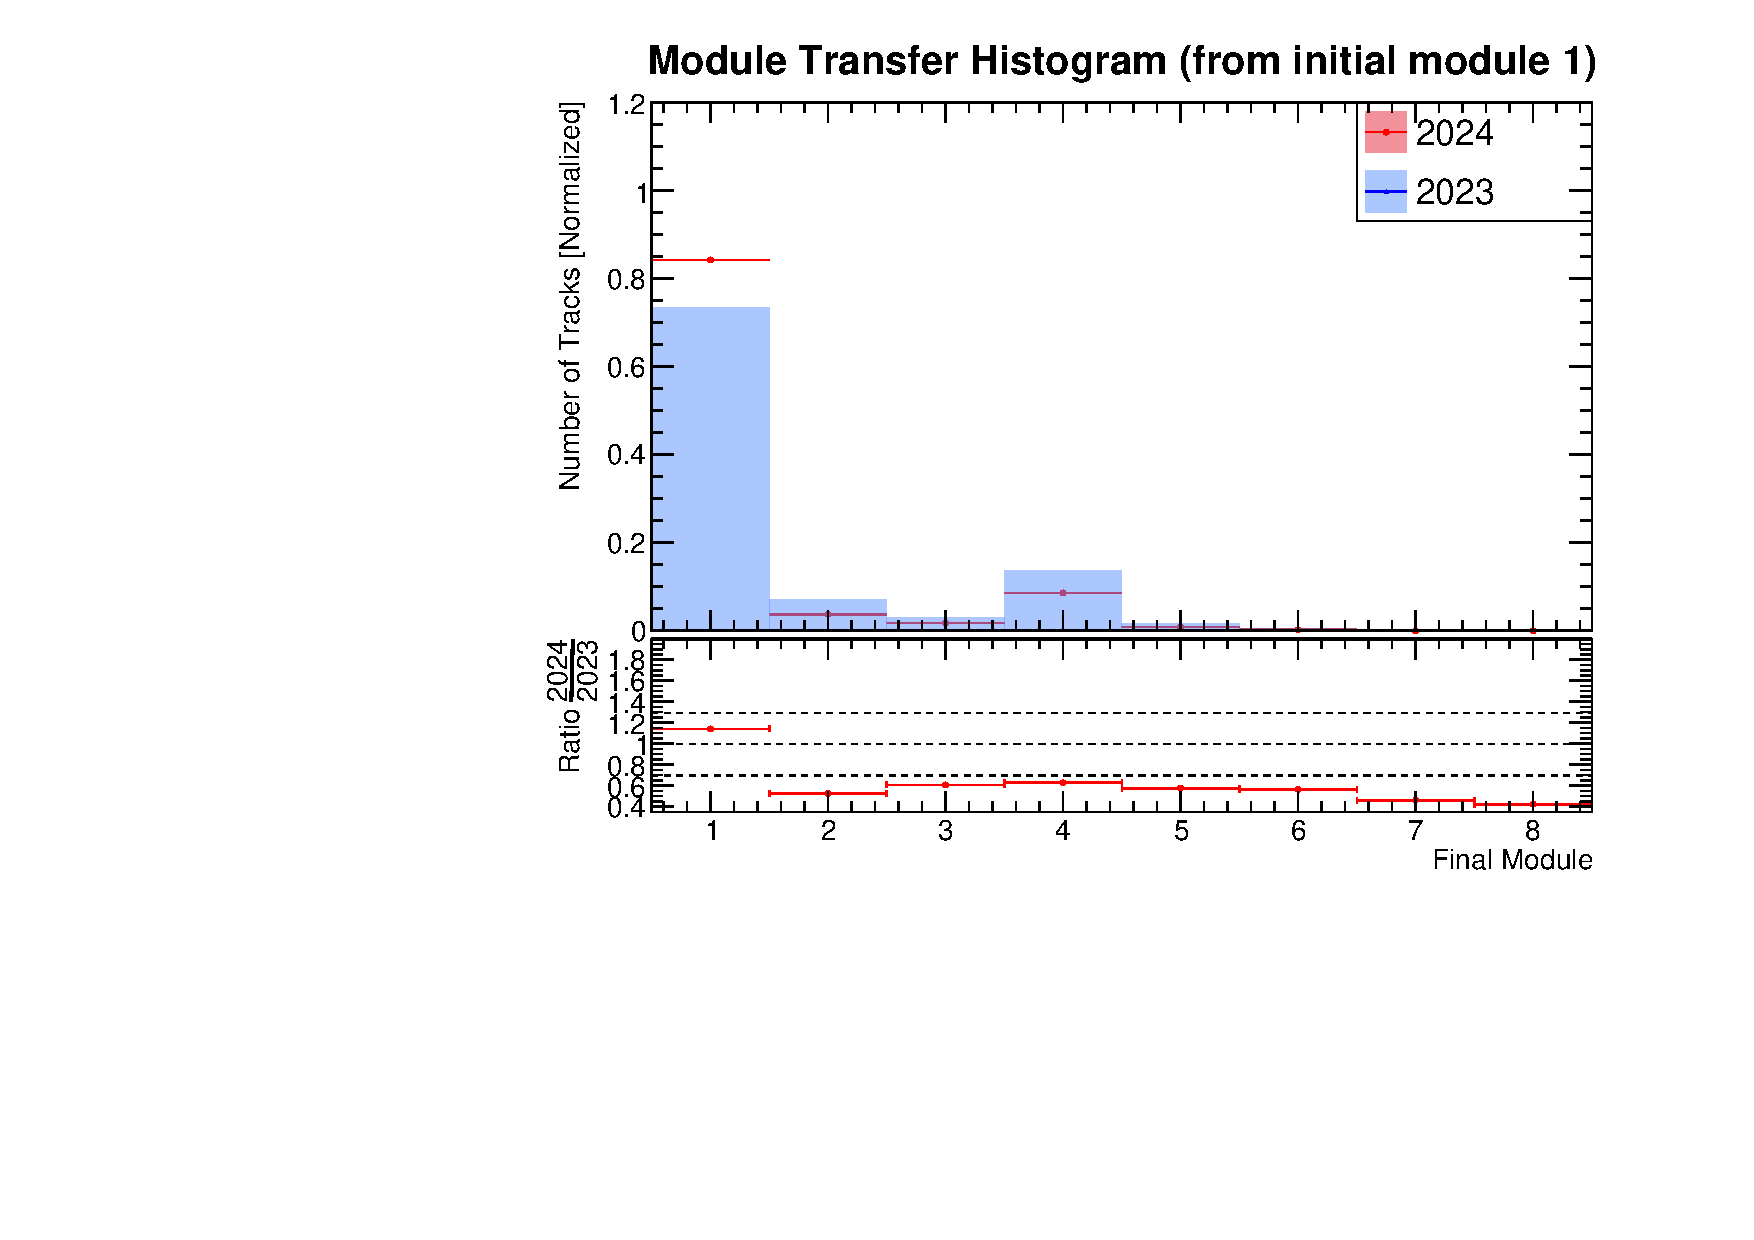
\includegraphics[width=\linewidth]{./ModuleLevelPlots/final_module_from_st0_module1.pdf}
%         \end{subfigure}
%         \begin{subfigure}[t]{0.49\linewidth}
%             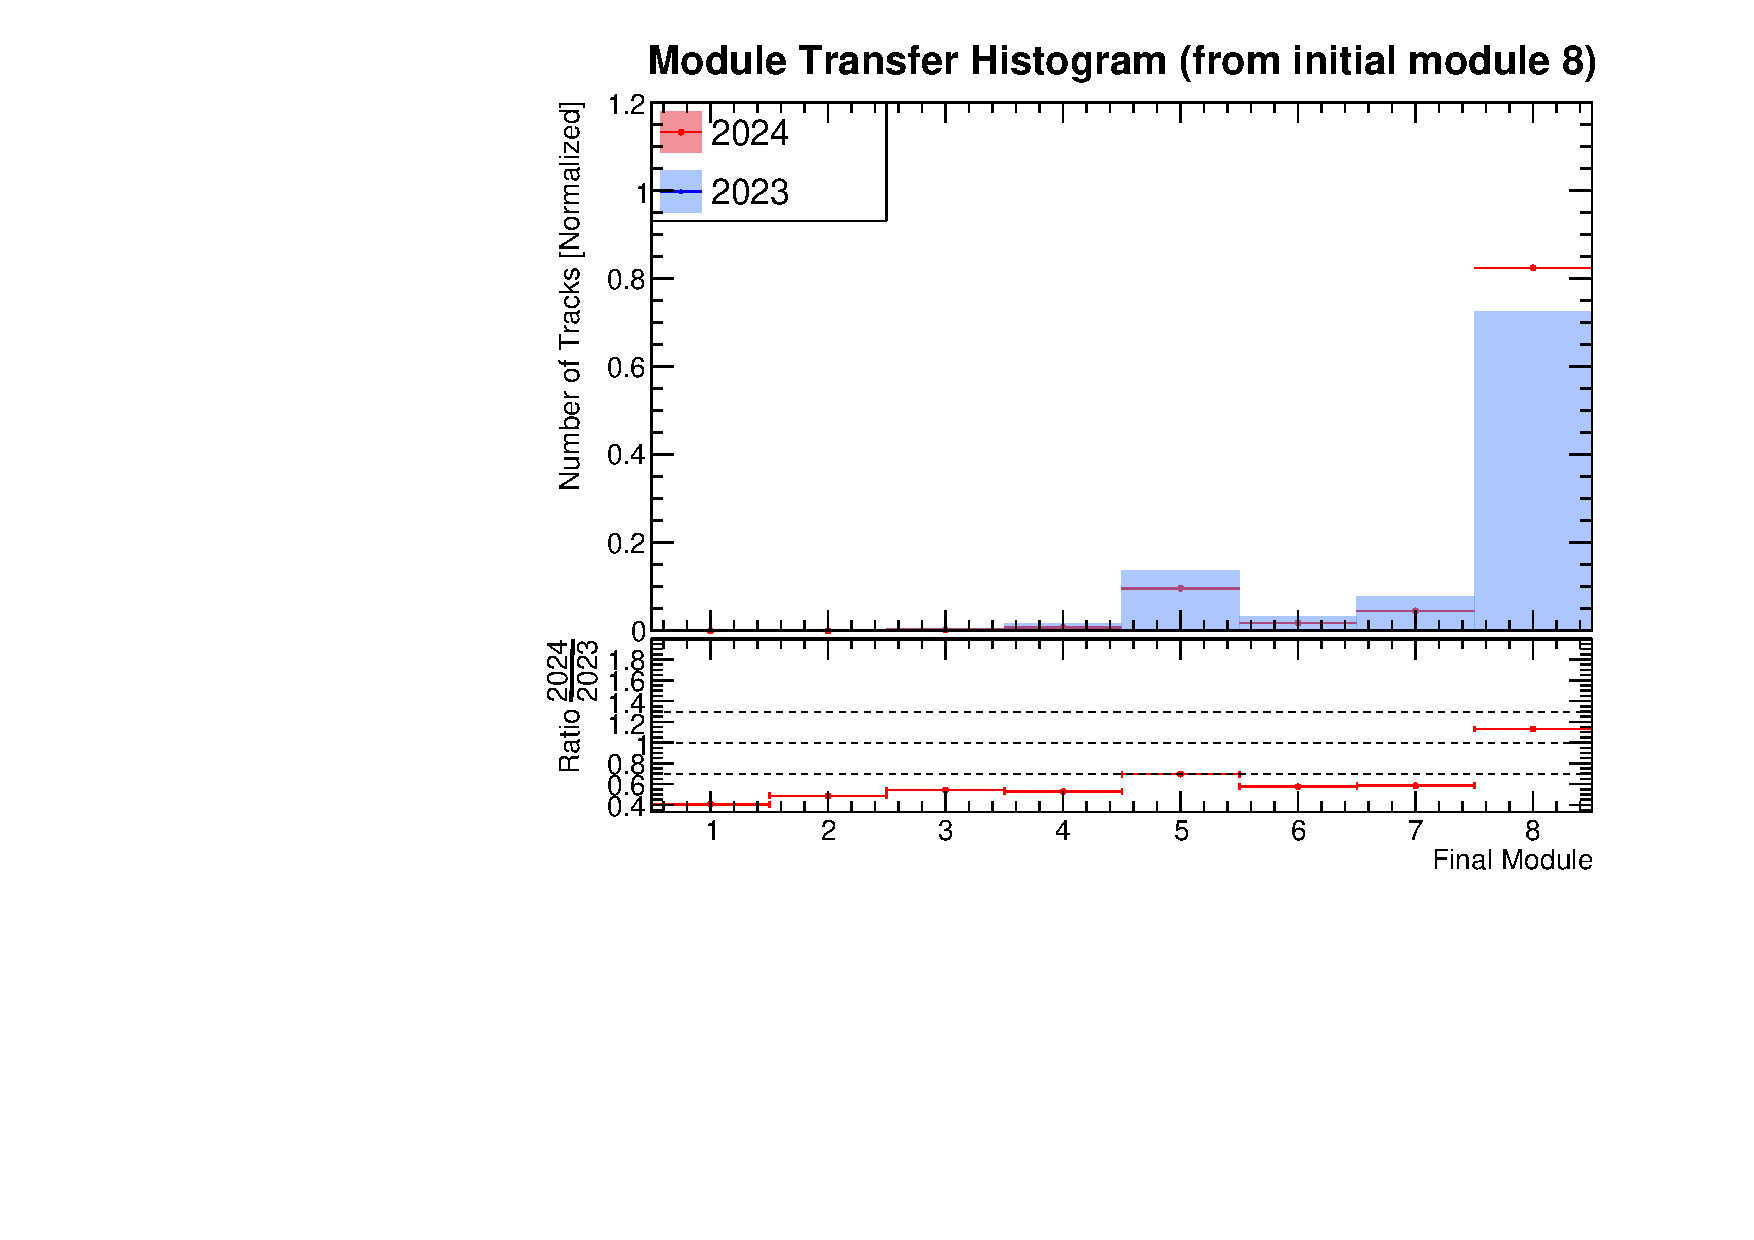
\includegraphics[width=\linewidth]{./ModuleLevelPlots/final_module_from_st0_module8.pdf}
%         \end{subfigure}

%         \begin{subfigure}[t]{0.49\linewidth}
%             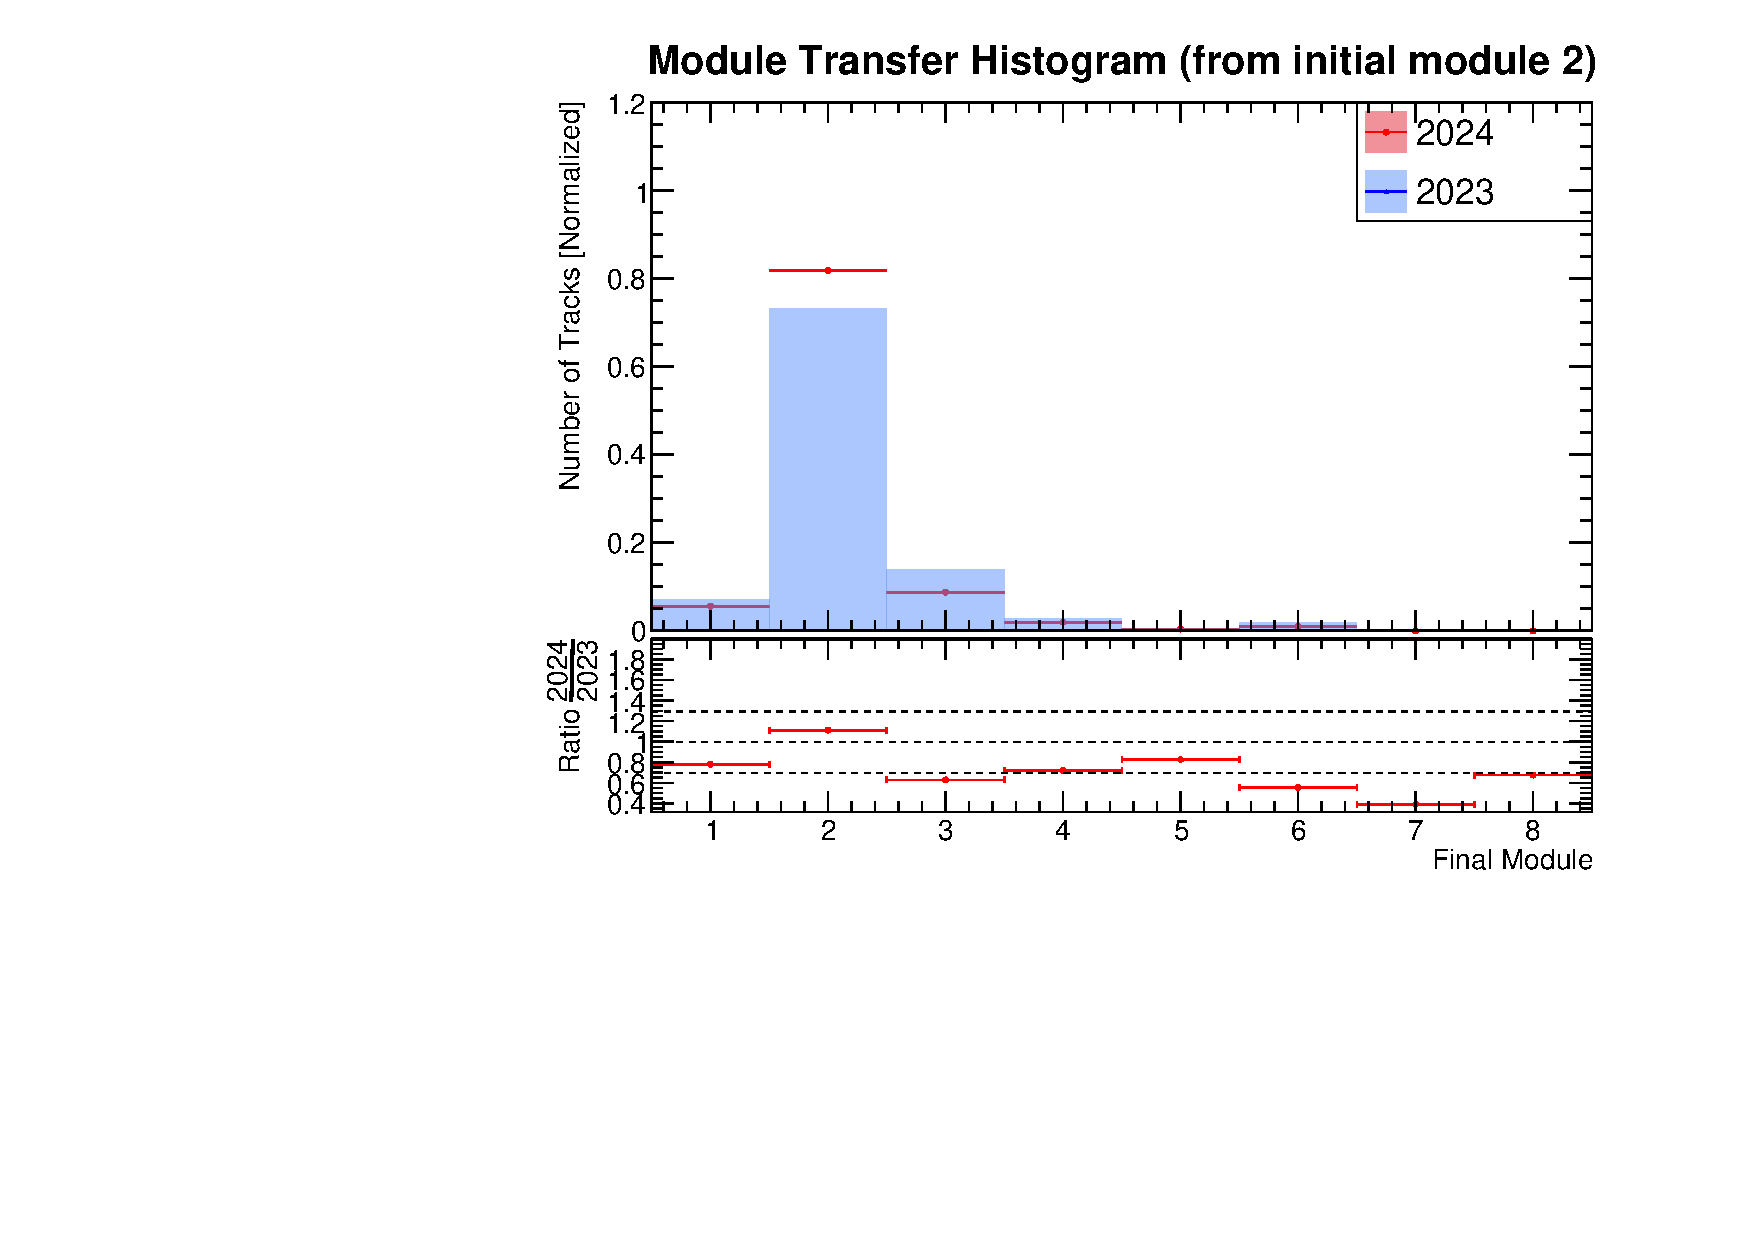
\includegraphics[width=\linewidth]{./ModuleLevelPlots/final_module_from_st0_module2.pdf}
%         \end{subfigure}
%         \begin{subfigure}[t]{0.49\linewidth}
%             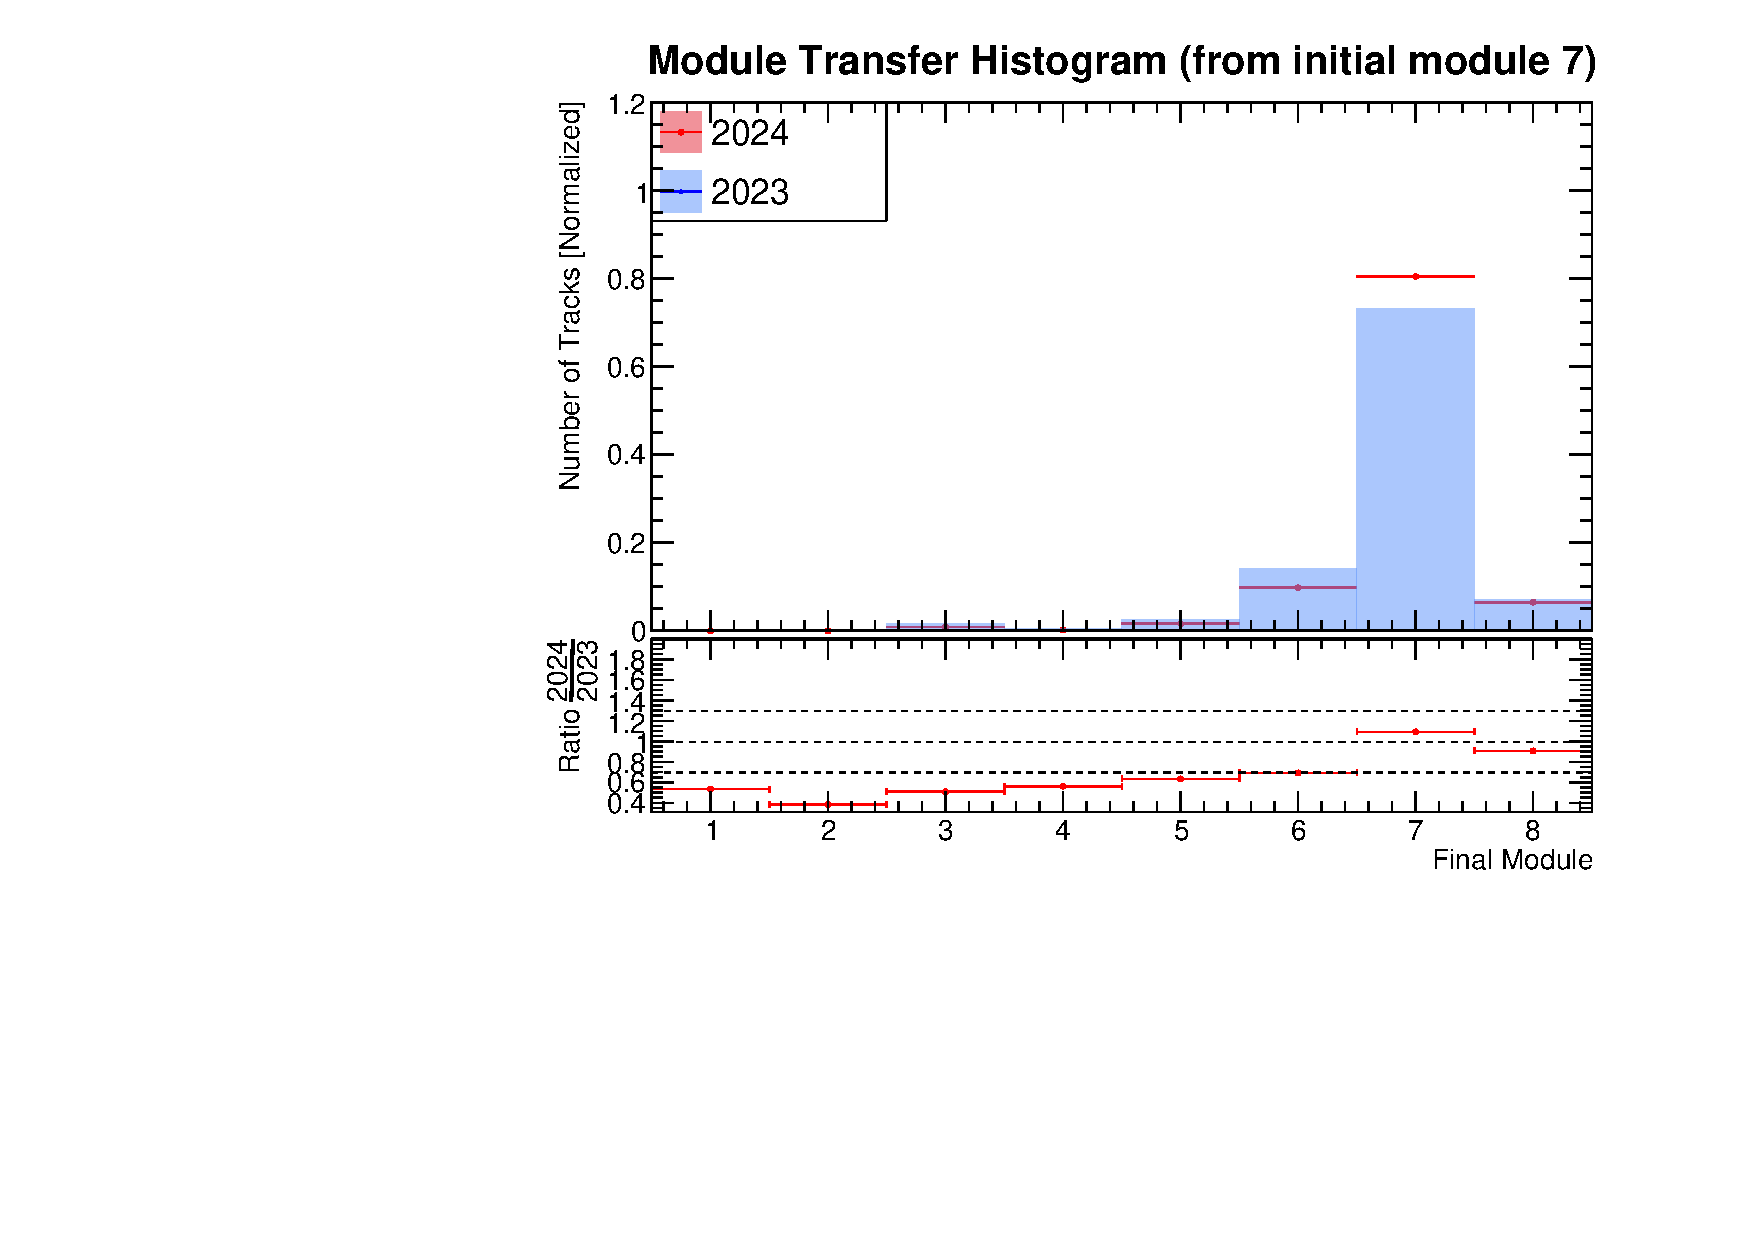
\includegraphics[width=\linewidth]{./ModuleLevelPlots/final_module_from_st0_module7.pdf}
%         \end{subfigure}
%     \end{figure}
%     \vspace{-0.3cm}
%     \scriptsize Note: 1-4 transfer seem significant? and 8-5 transfer seem significant?
% \end{frame}

% \begin{frame}{Transfer Histograms [Contd.]}
%     \begin{figure}
%         \centering
%         \begin{subfigure}[t]{0.49\linewidth}
%             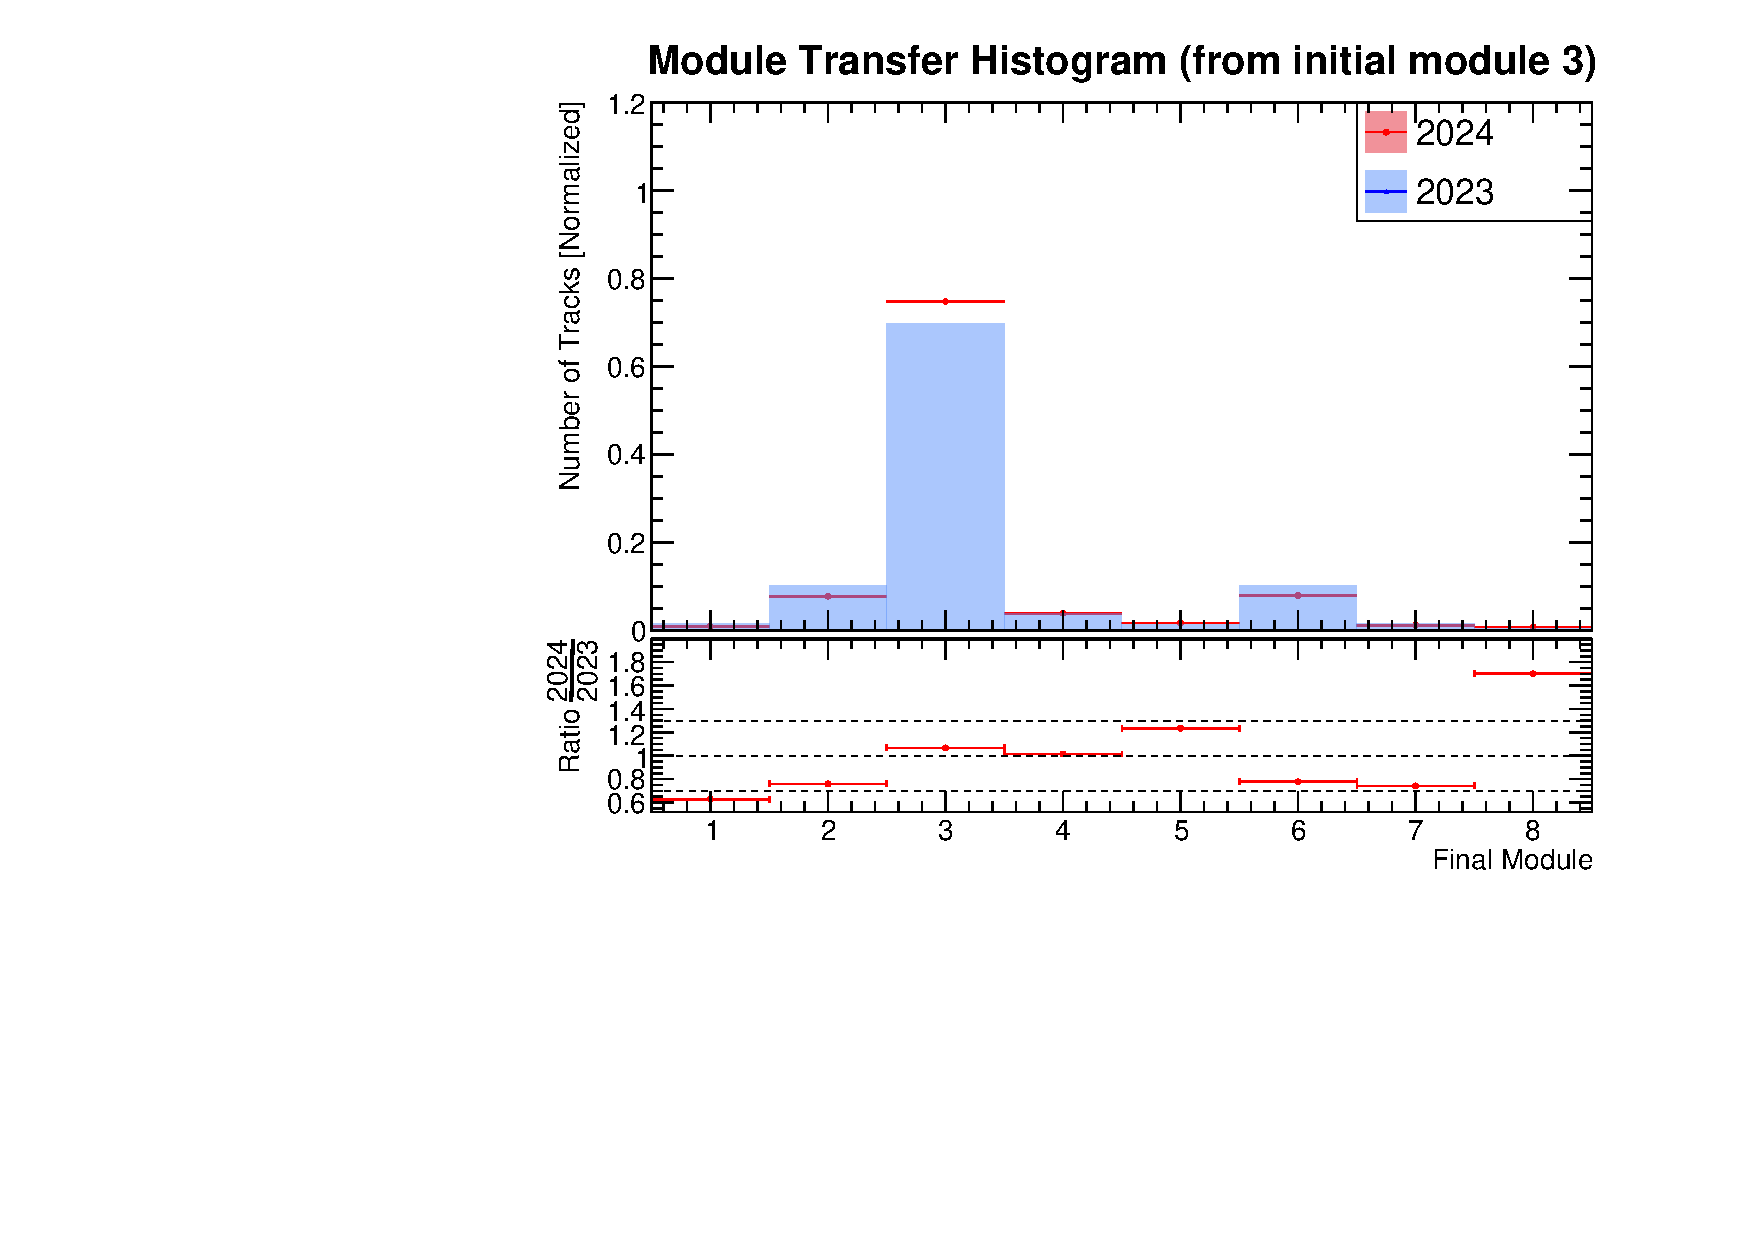
\includegraphics[width=\linewidth]{./ModuleLevelPlots/final_module_from_st0_module3.pdf}
%         \end{subfigure}
%         \begin{subfigure}[t]{0.49\linewidth}
%             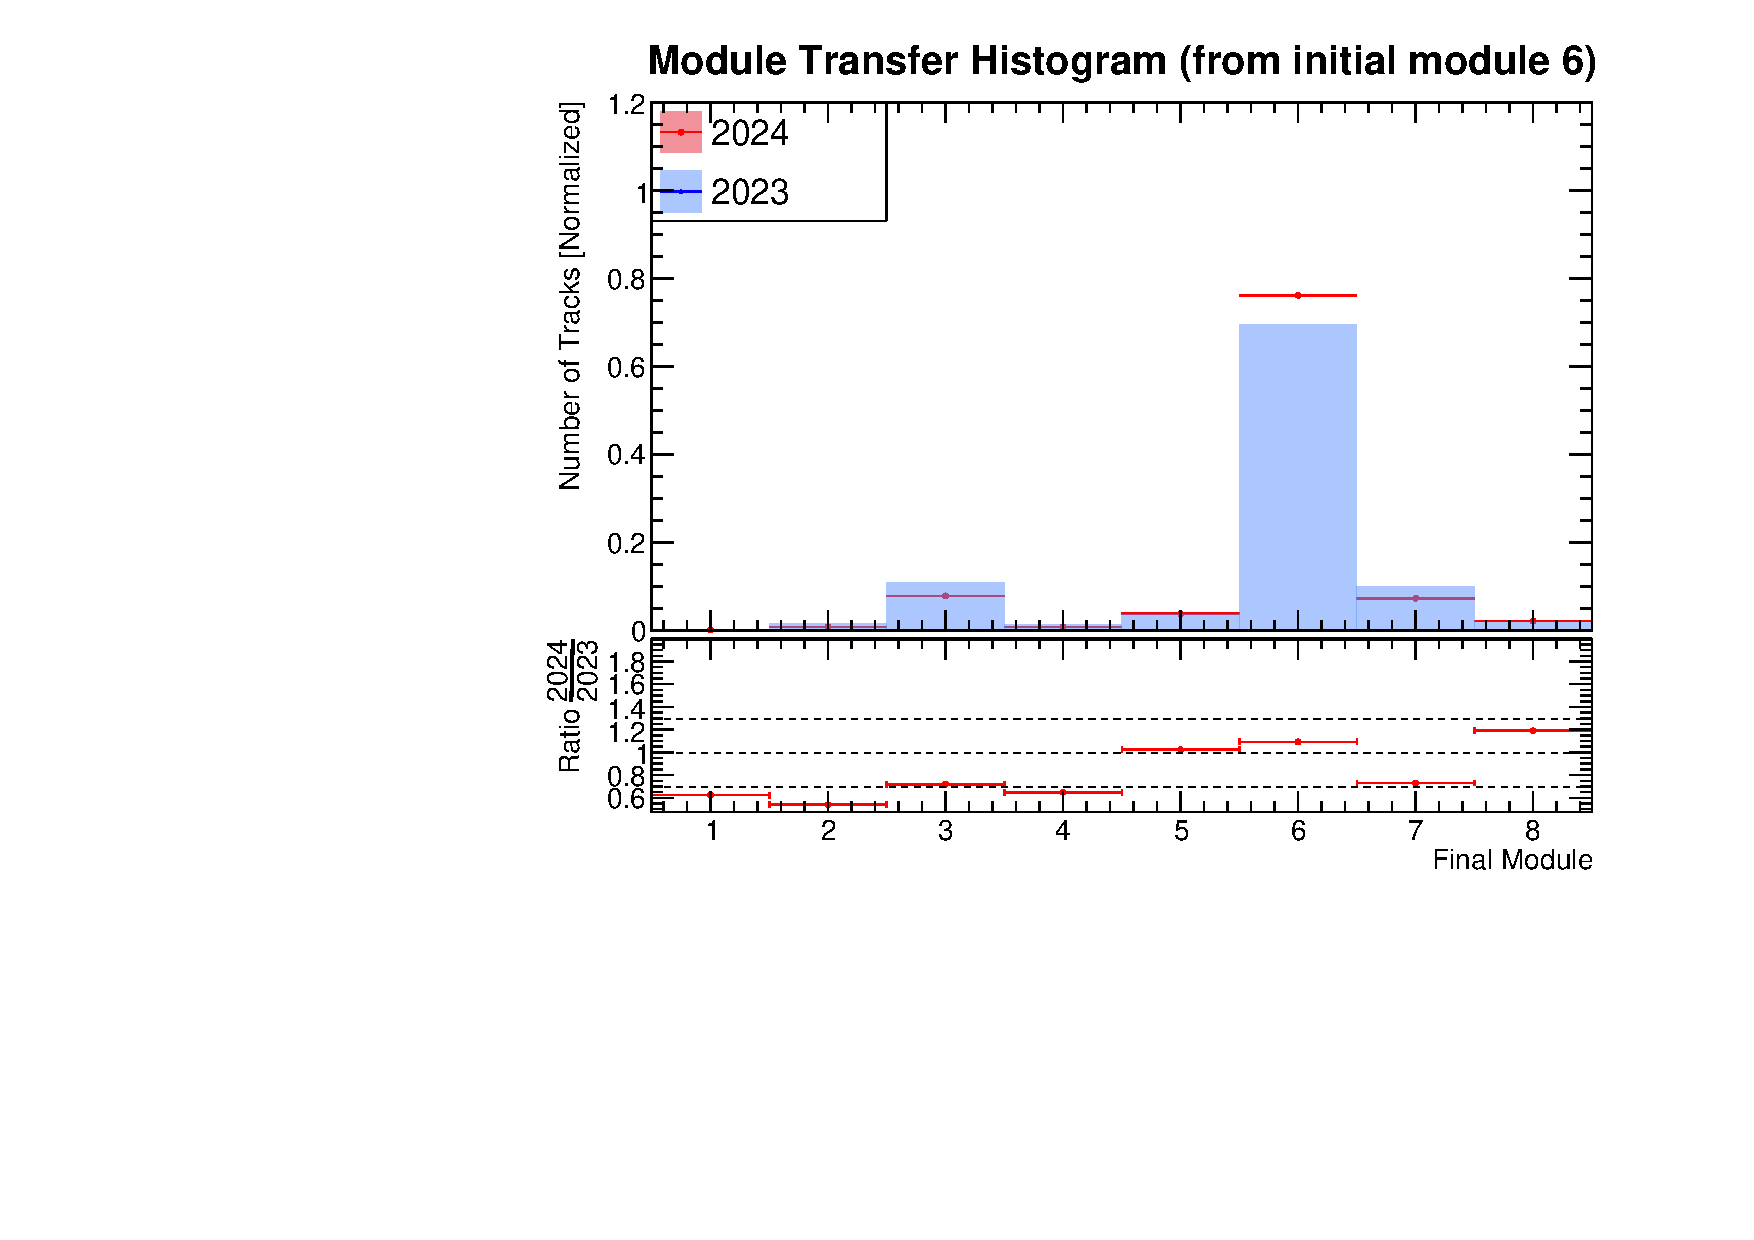
\includegraphics[width=\linewidth]{./ModuleLevelPlots/final_module_from_st0_module6.pdf}
%         \end{subfigure}

%         \begin{subfigure}[t]{0.49\linewidth}
%             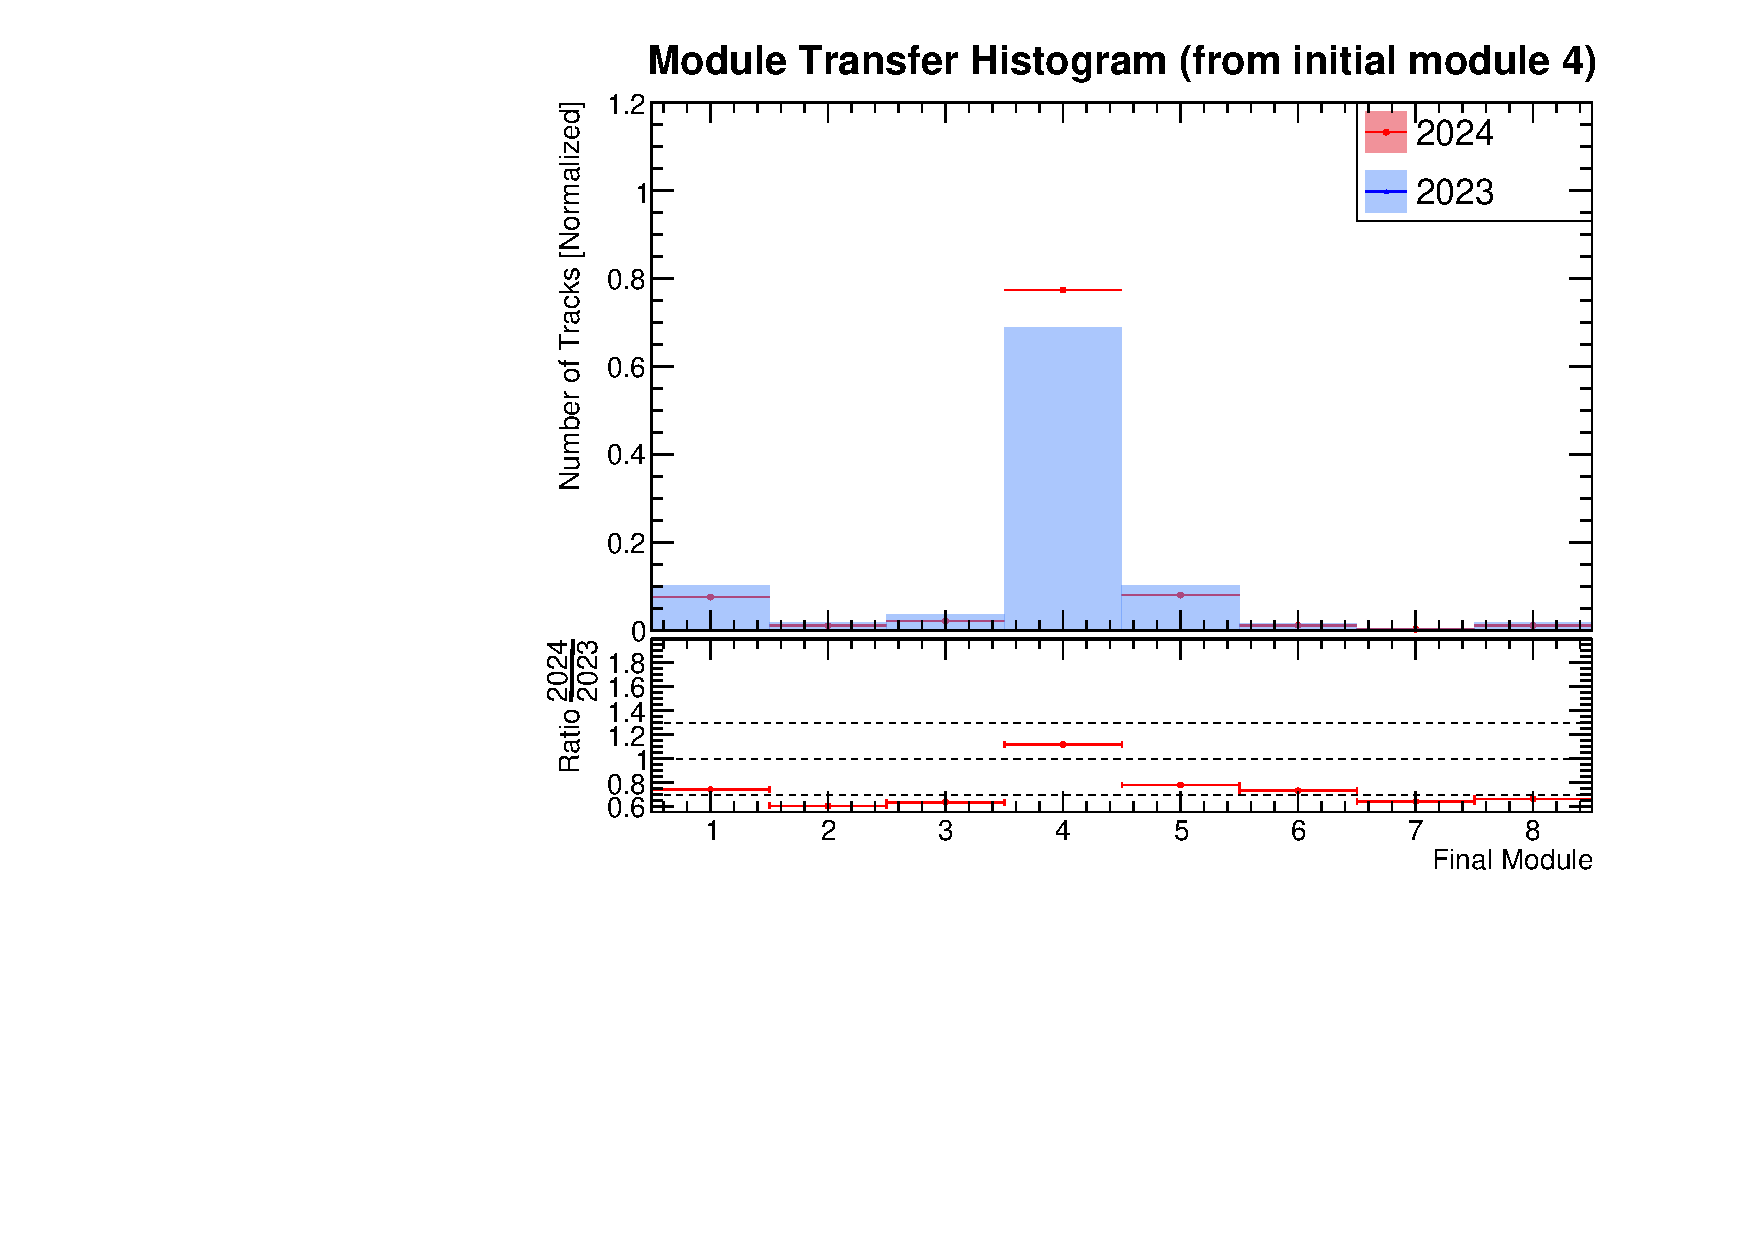
\includegraphics[width=\linewidth]{./ModuleLevelPlots/final_module_from_st0_module4.pdf}
%         \end{subfigure}
%         \begin{subfigure}[t]{0.49\linewidth}
%             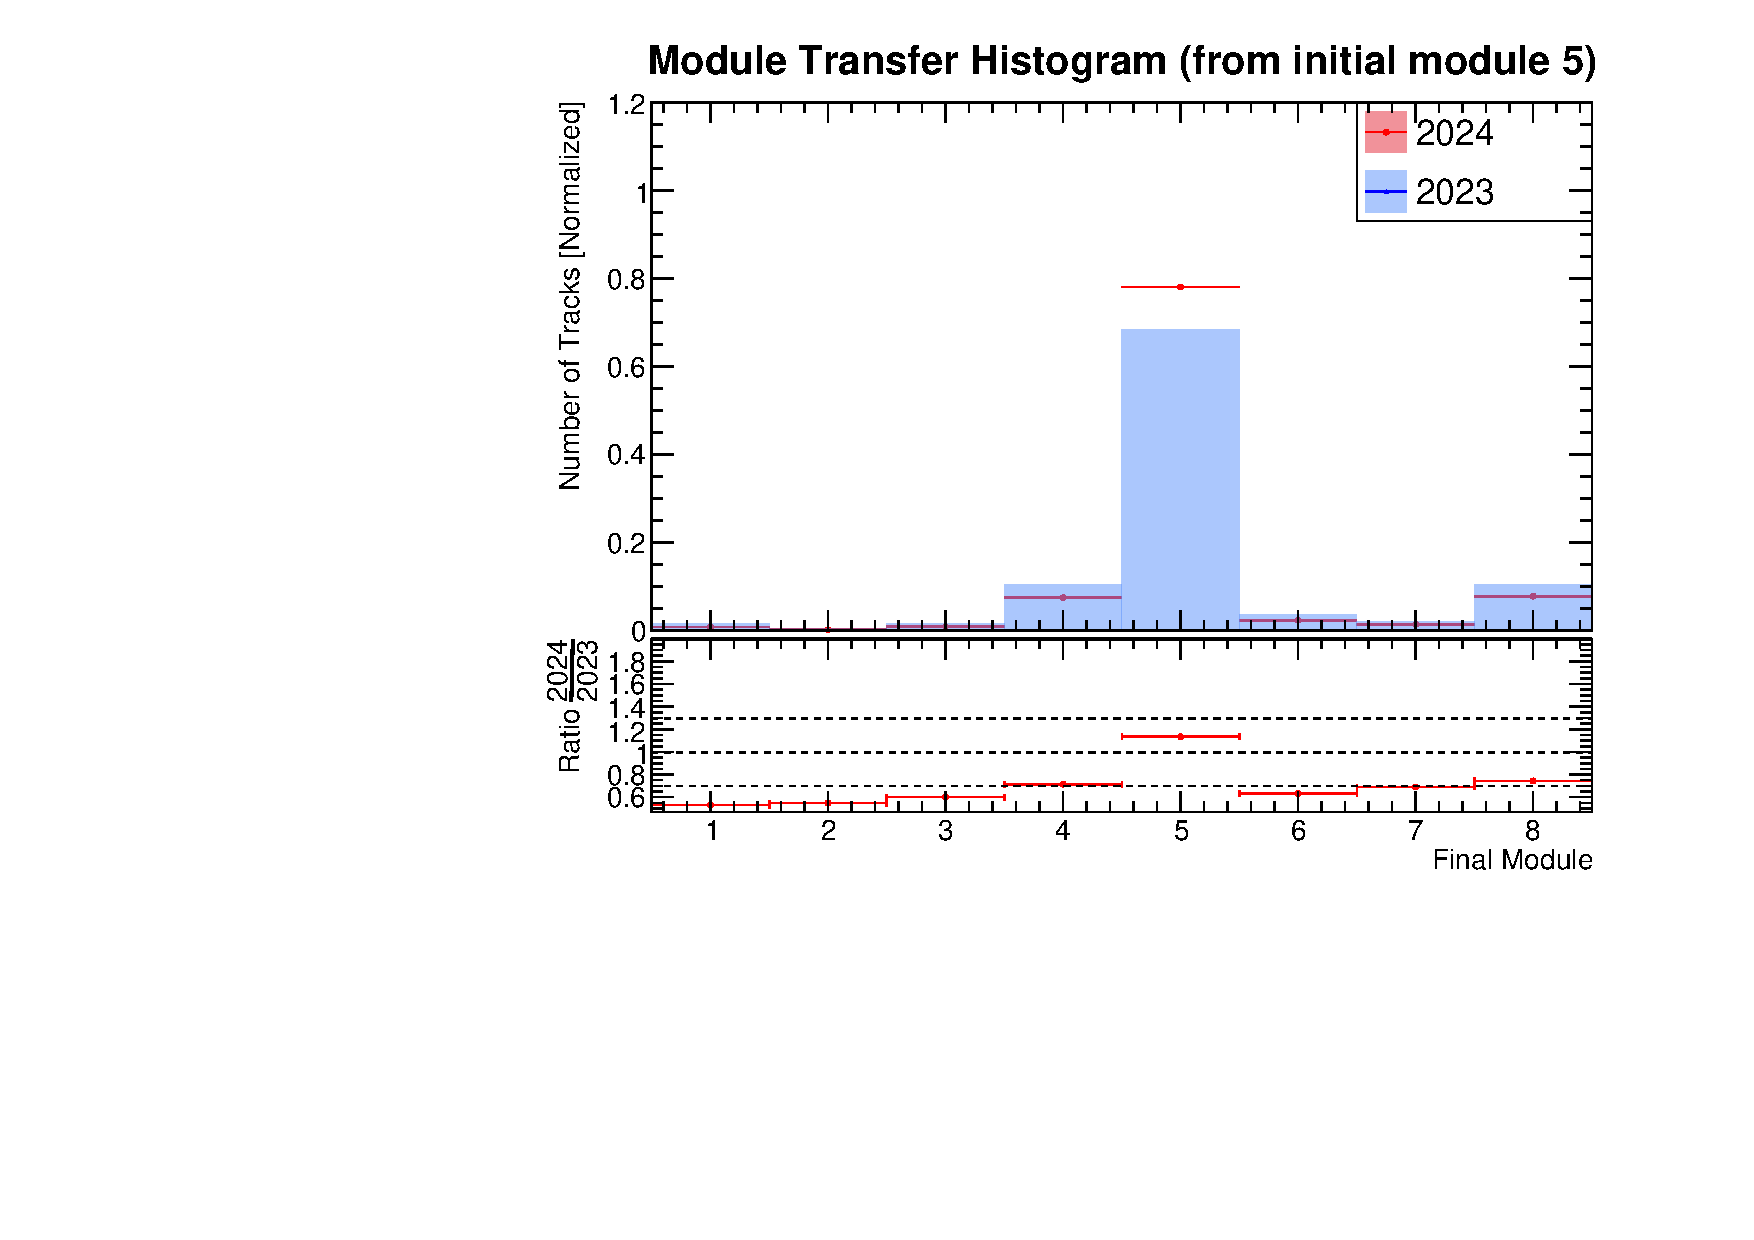
\includegraphics[width=\linewidth]{./ModuleLevelPlots/final_module_from_st0_module5.pdf}
%         \end{subfigure}
%     \end{figure}
% \end{frame}

% \section{Track Parameters Modulewise}    

\begin{frame}{Modulewise Track Parameters}
    
    \begin{itemize}
        \item The module\_eta0/phi0 variables exist only in the 2024 data
        \item For uniformity we define the module numbers using the x and y positions for both the 2023 and 2024 data
        \item The agreement is not good, both module-wise or year-wise.
        \item Possibly from the Momenta being different between them
        \item Although modules tend to group together for some parameters based on their relative position.
    \end{itemize}
    % Recap of the Track Parameters:
    % \begin{itemize}
    %     \item Number of longTracks
    %     \item Track Charge
    %     \item TracK Momenta 
    %     \item Track Chi2 
    %     \item Track nDoF
    %     \item Track Chi2perDoF [SKIP]
    %     \item Track In Station [SKIP]
    %     \item Track nLayers [SKIP]
    %     \item Track Propagation Error [SKIP]
    % \end{itemize}
    \vspace{0.3 cm}
    \small{    
    \textbf{Note:} Unfortunately, 8 modules across 2 year = 16 Histograms \\
    An year wise for each module would be too long.
    So we do a module level comparison, year wise plots available in the slides linked to in backup.\\ 
    
    Module transfer plots are also available in the detailed slides in the backup.  
    }
    % \begin{itemize}
    %     \item Hard to visualize, so we do a module level comparison
    %     \item More detailed plots available in the backup/repo
    % \end{itemize}
\end{frame}




\newcommand{\makemodulewiseframes}[2]{
    \begin{frame}{#2}
        \newcommand{\colname}{#1}
        \begin{figure}
            \centering
            \begin{subfigure}[t]{0.49\linewidth}
                \includegraphics[width=\linewidth]{./ModuleLevelPlots/\colname_st0_module1.pdf}
            \end{subfigure}
            \begin{subfigure}[t]{0.49\linewidth}
                \includegraphics[width=\linewidth]{./ModuleLevelPlots/\colname_st0_module8.pdf}
            \end{subfigure}
    
            \begin{subfigure}[t]{0.49\linewidth}
                \includegraphics[width=\linewidth]{./ModuleLevelPlots/\colname_st0_module2.pdf}
            \end{subfigure}
            \begin{subfigure}[t]{0.49\linewidth}
                \includegraphics[width=\linewidth]{./ModuleLevelPlots/\colname_st0_module7.pdf}
            \end{subfigure}
        \end{figure}
    \end{frame}
    \begin{frame}{#2 [Contd.]}
        \newcommand{\colname}{#1}
        \begin{figure}
            \centering
            \begin{subfigure}[t]{0.49\linewidth}
                \includegraphics[width=\linewidth]{./ModuleLevelPlots/\colname_st0_module3.pdf}
            \end{subfigure}
            \begin{subfigure}[t]{0.49\linewidth}
                \includegraphics[width=\linewidth]{./ModuleLevelPlots/\colname_st0_module6.pdf}
            \end{subfigure}
    
            \begin{subfigure}[t]{0.49\linewidth}
                \includegraphics[width=\linewidth]{./ModuleLevelPlots/\colname_st0_module4.pdf}
            \end{subfigure}
            \begin{subfigure}[t]{0.49\linewidth}
                \includegraphics[width=\linewidth]{./ModuleLevelPlots/\colname_st0_module5.pdf}
            \end{subfigure}
        \end{figure}
    \end{frame}

}



% \makemodulewiseframes{longTracks}{Distribution longTracks Modulewise}
% \begin{frame}{Distribution longTracks Modulewise}
%     \newcommand{\colname}{longTracks}
%     \begin{columns}
%         \begin{column}{0.6\linewidth}
%             \begin{figure}
%                 \centering
%                 \includegraphics[width=\linewidth]{./ModuleLevelPlots/\colname_st0_2023.pdf}
%             \end{figure}
%         \end{column}
%         \begin{column}{0.6\linewidth}
%             \begin{figure}
%                 \centering
%                 \includegraphics[width=\linewidth]{./ModuleLevelPlots/\colname_st0_2024.pdf}
%             \end{figure}
%         \end{column}
%     \end{columns}
%     \begin{itemize}
%         \item 2024 has more events in the tail
%         \item Seem to form two groups with [for other Parameters as well]
%         \begin{itemize}
%             \item Modules 2,7,8 having lower long tracks [pronounced in bin2]
%             \item Separation between groups worse with higher longTracks
%         \end{itemize}
%     \end{itemize}
% \end{frame}


% \makemodulewiseframes{Track_Chi2}{Track Chi2 Modulewise}
% \begin{frame}{Track Chi2 Modulewise}
%     \newcommand{\colname}{Track_Chi2}
%     \begin{columns}
%         \begin{column}{0.6\linewidth}
%             \begin{figure}
%                 \centering
%                 \includegraphics[width=\linewidth]{./ModuleLevelPlots/\colname_st0_2023.pdf}
%             \end{figure}
%         \end{column}
%         \begin{column}{0.6\linewidth}
%             \begin{figure}
%                 \centering
%                 \includegraphics[width=\linewidth]{./ModuleLevelPlots/\colname_st0_2024.pdf}
%             \end{figure}
%         \end{column}
%     \end{columns}

%     \begin{itemize}
%         \small
%         \item Better Agreement in 2024 amongst modules
%         \item Module 2 shows higher Track Chi2 in 2023
%     \end{itemize}
% \end{frame}

% \makemodulewiseframes{Track_nDoF}{Track Degrees of Freedom Modulewise}
% \begin{frame}{Track Degrees of Freedom Modulewise}
%     \newcommand{\colname}{Track_nDoF}
%     \begin{columns}
%         \begin{column}{0.6\linewidth}
%             \begin{figure}
%                 \centering
%                 \includegraphics[width=\linewidth]{./ModuleLevelPlots/\colname_st0_2023.pdf}
%             \end{figure}
%         \end{column}
%         \begin{column}{0.6\linewidth}
%             \begin{figure}
%                 \centering
%                 \includegraphics[width=\linewidth]{./ModuleLevelPlots/\colname_st0_2024.pdf}
%             \end{figure}
%         \end{column}
%     \end{columns}

%     \begin{itemize}
%         \small
%         \item Module 2 has significantly higher nDoF in 2024
%         \item In 2024 more tracks have nDof $\geq 20$
%         \item Track NDoF split into two groups
%         \begin{itemize}
%             \item Higher nDoF Modules : 2, 1, 8, 7 [Modules with y $\geq$ 0]
%             \item Lower nDoF Modules \ : 3, 4, 5, 6  [Modules with y $\leq$ 0]
%         \end{itemize}
%     \end{itemize}
% \end{frame}

% \makemodulewiseframes{Track_Chi2perDoF}{Track Chi2perDoF Modulewise}
% \begin{frame}{Track Chi2perDoF Modulewise}
%     \newcommand{\colname}{Track_Chi2perDoF}
%     \begin{columns}
%         \begin{column}{0.6\linewidth}
%             \begin{figure}
%                 \centering
%                 \includegraphics[width=\linewidth]{./ModuleLevelPlots/\colname_st0_2023.pdf}
%             \end{figure}
%         \end{column}
%         \begin{column}{0.6\linewidth}
%             \begin{figure}
%                 \centering
%                 \includegraphics[width=\linewidth]{./ModuleLevelPlots/\colname_st0_2024.pdf}
%             \end{figure}
%         \end{column}
%     \end{columns}

%     \begin{itemize}
%         \small
%         \item In 2023, the Track Chi2 seem to split into two groups
%         \begin{itemize}
%             \item Higher Chi2 Modules : 2, 1, 8, 7 [Modules with y $\geq$ 0]
%             \item Lower Chi2 Modules \ : 3, 4, 5, 6  [Modules with y $\leq$ 0]
%         \end{itemize}
%     \end{itemize}
% \end{frame}

% \makemodulewiseframes{Track_nLayers}{Distribution of Track\_nLayers Modulewise}
% \begin{frame}{Distribution of Track\_nLayers Modulewise}
%     \newcommand{\colname}{Track_nLayers}
%     \begin{columns}
%         \begin{column}{0.6\linewidth}
%             \begin{figure}
%                 \centering
%                 \includegraphics[width=\linewidth]{./ModuleLevelPlots/\colname_st0_2023.pdf}
%             \end{figure}
%         \end{column}
%         \begin{column}{0.6\linewidth}
%             \begin{figure}
%                 \centering
%                 \includegraphics[width=\linewidth]{./ModuleLevelPlots/\colname_st0_2024.pdf}
%             \end{figure}
%         \end{column}
%     \end{columns}

%     \begin{itemize}
%         \small
%         \item Again seem to split into two groups
%         \begin{itemize}
%             \item Higher nLayer Modules : 2, 1, 8, 7 [Modules with y $\geq$ 0]
%             \item Lower nLayer Modules \ : 3, 4, 5, 6  [Modules with y $\leq$ 0]
%         \end{itemize}
%     \end{itemize}
% \end{frame}

% \begin{frame}{Track Momenta Modulewise}
%     \begin{figure}
%         \centering
%         \begin{subfigure}[t]{0.49\linewidth}
%             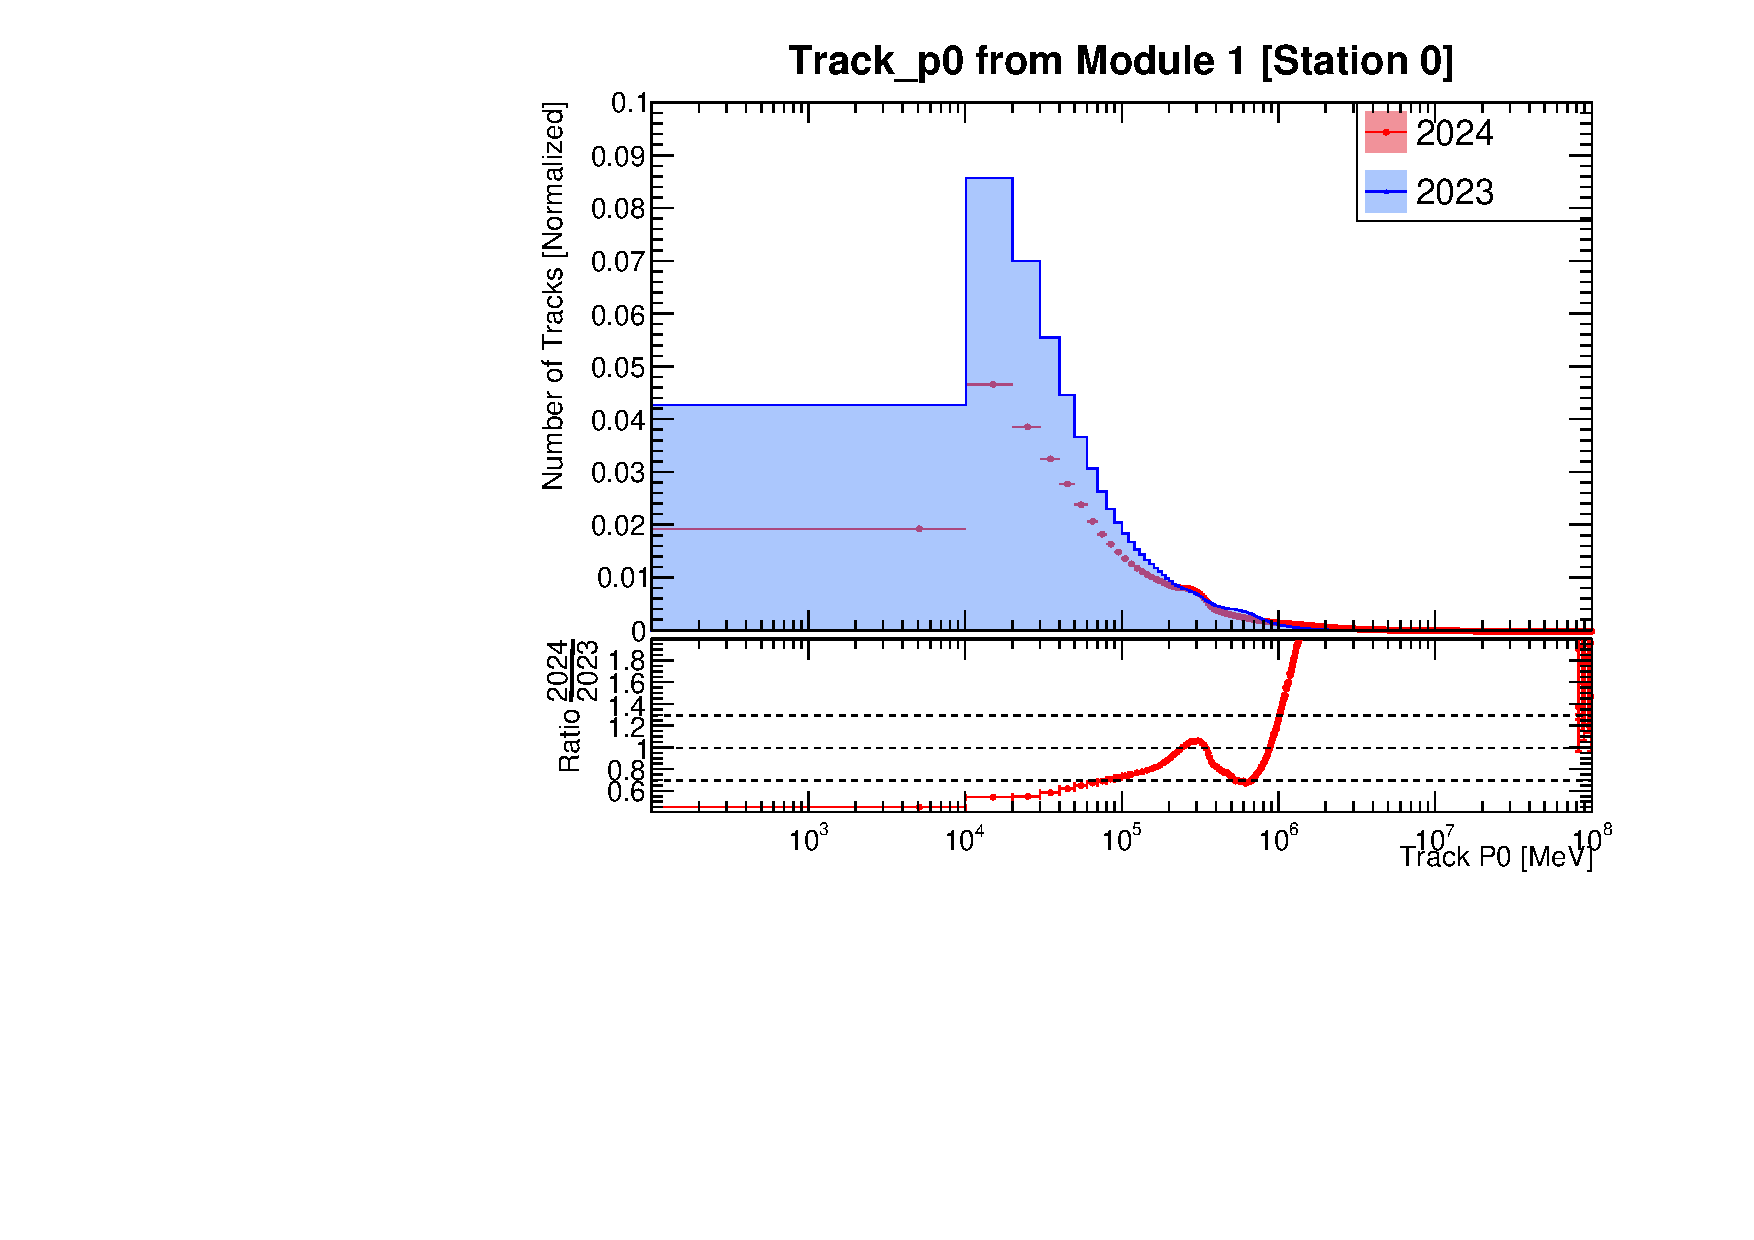
\includegraphics[width=\linewidth]{./ModuleLevelPlots/Track_p0_st0_module1_linear.pdf}
%         \end{subfigure}
%         \begin{subfigure}[t]{0.49\linewidth}
%             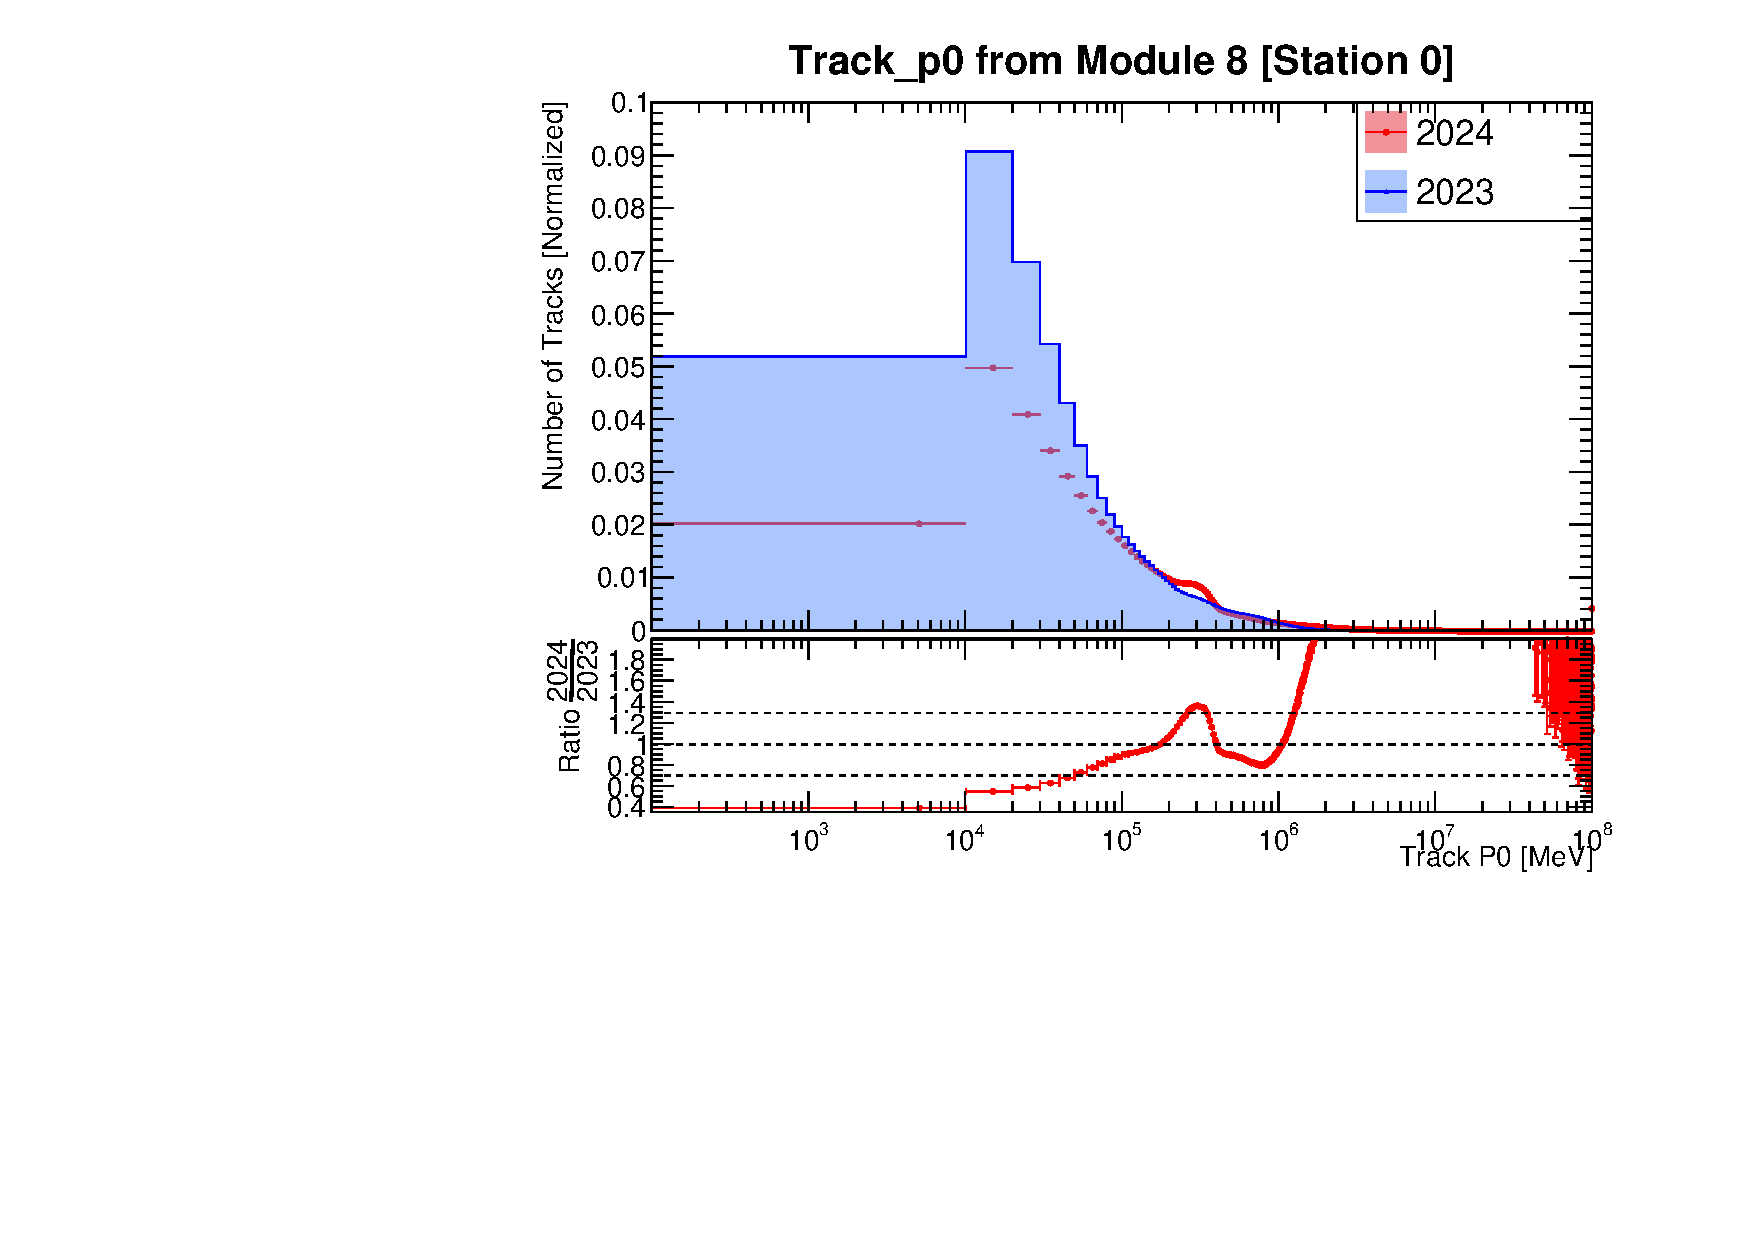
\includegraphics[width=\linewidth]{./ModuleLevelPlots/Track_p0_st0_module8_linear.pdf}
%         \end{subfigure}

%         \begin{subfigure}[t]{0.49\linewidth}
%             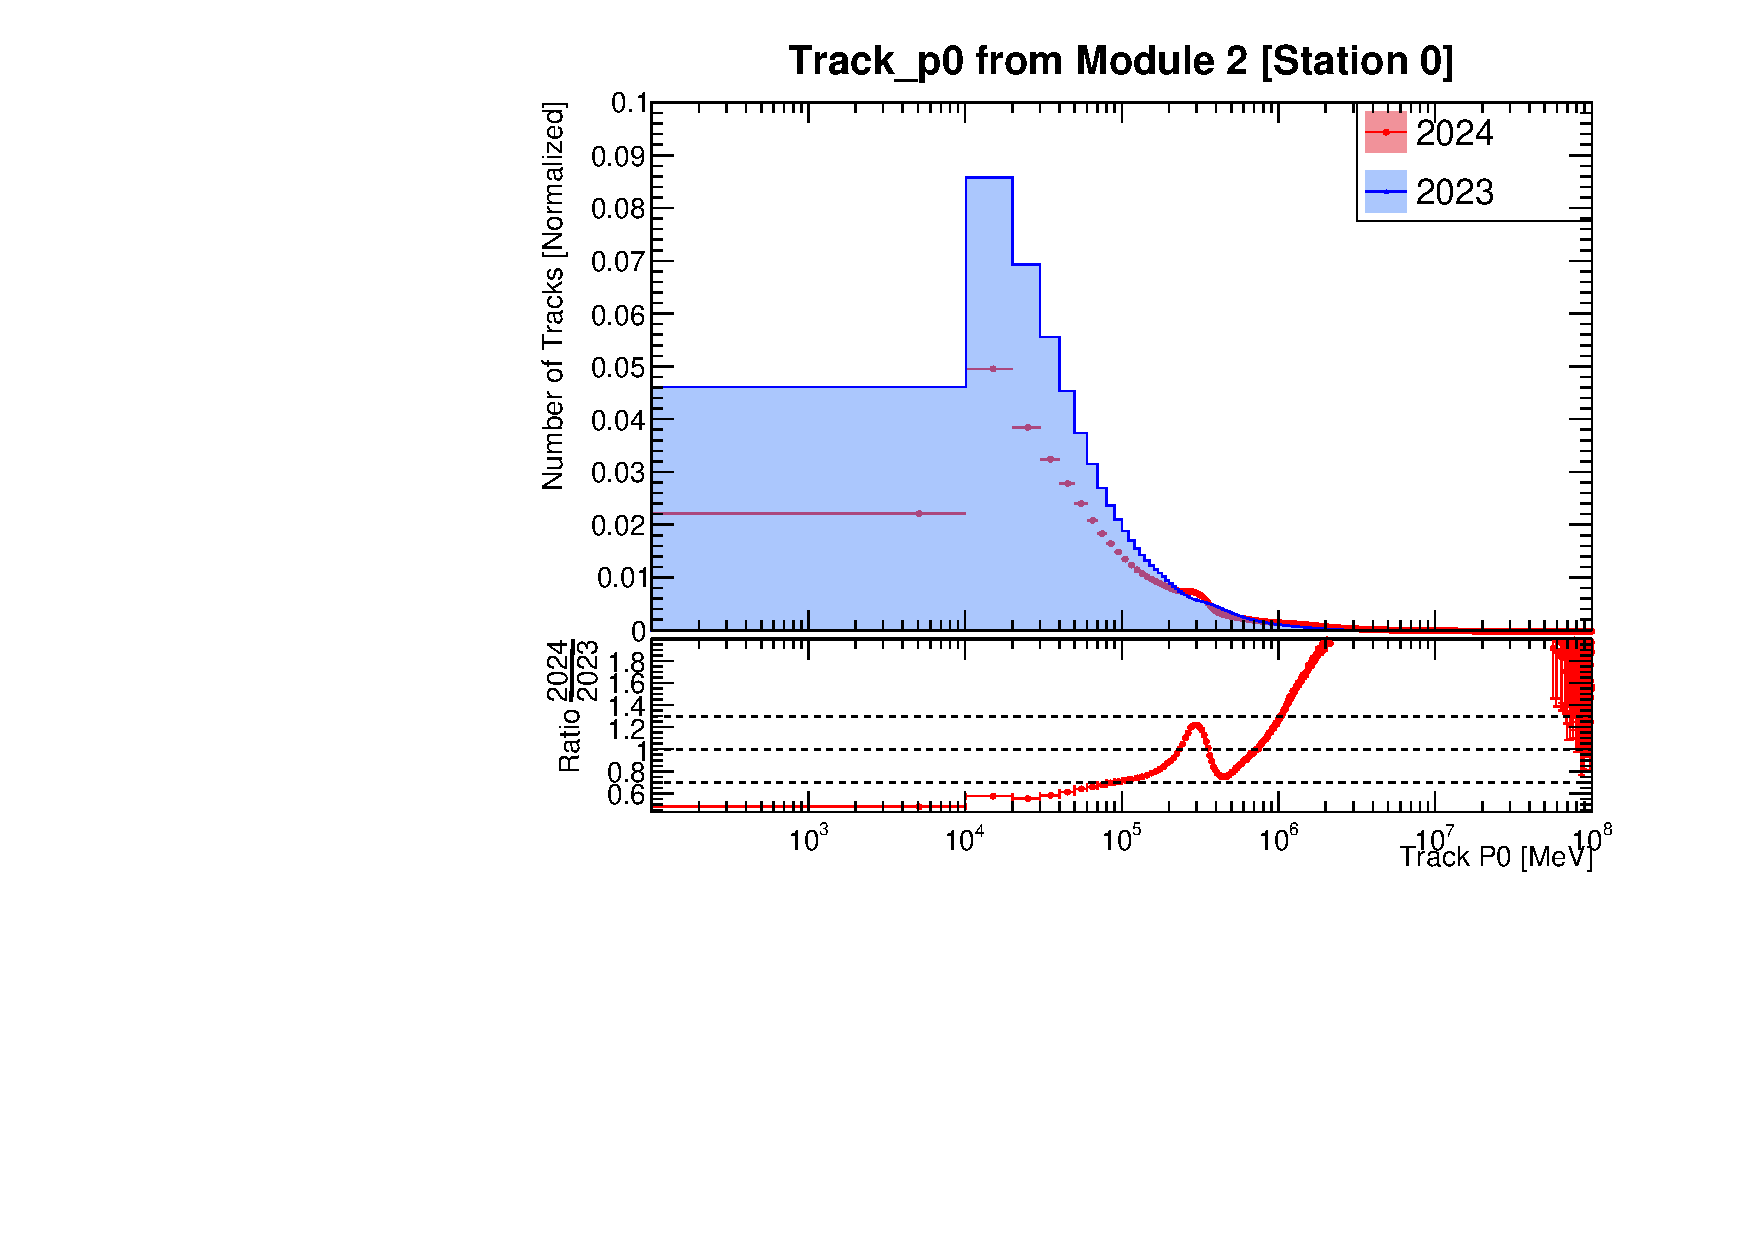
\includegraphics[width=\linewidth]{./ModuleLevelPlots/Track_p0_st0_module2_linear.pdf}
%         \end{subfigure}
%         \begin{subfigure}[t]{0.49\linewidth}
%             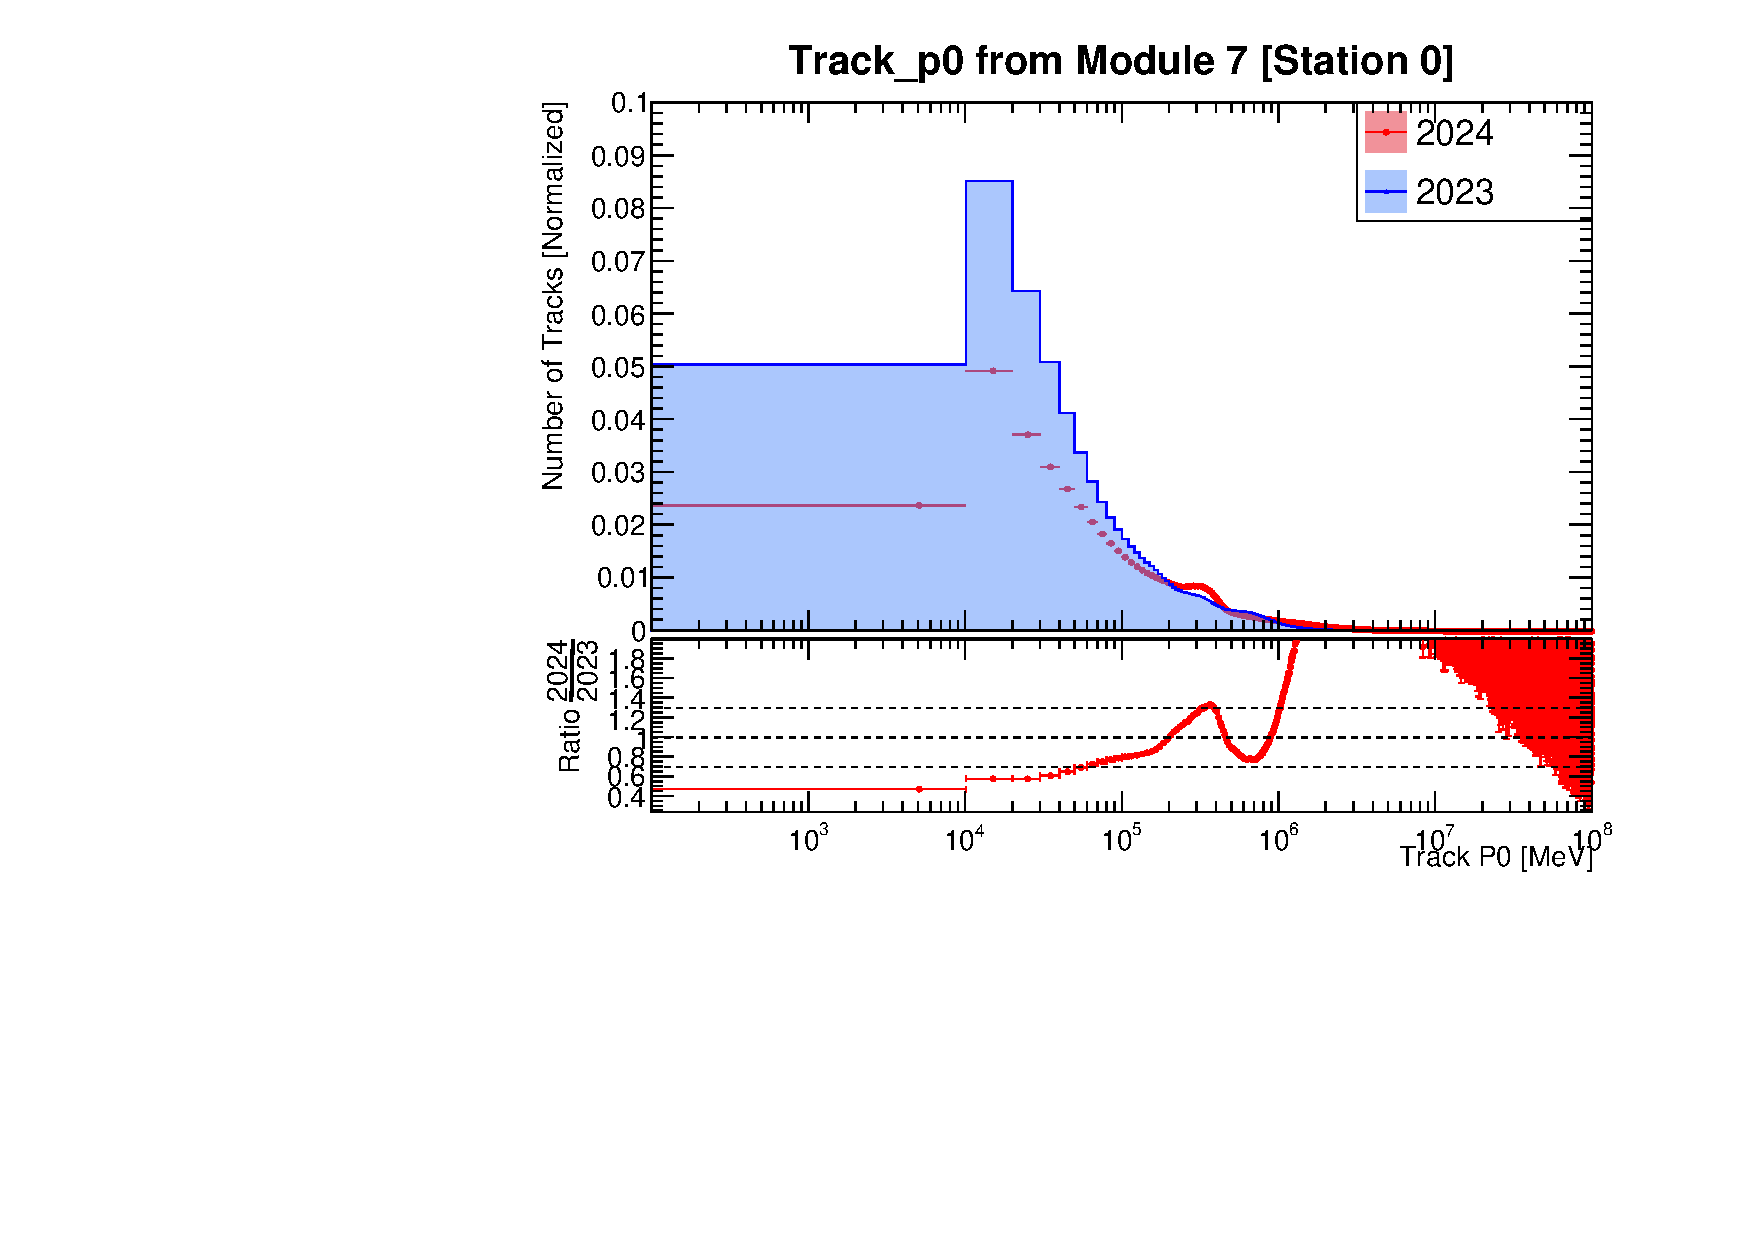
\includegraphics[width=\linewidth]{./ModuleLevelPlots/Track_p0_st0_module7_linear.pdf}
%         \end{subfigure}
%     \end{figure}
% \end{frame}

% \begin{frame}{Track Momenta Modulewise [Contd.]}
%     \begin{figure}
%         \centering
%         \begin{subfigure}[t]{0.49\linewidth}
%             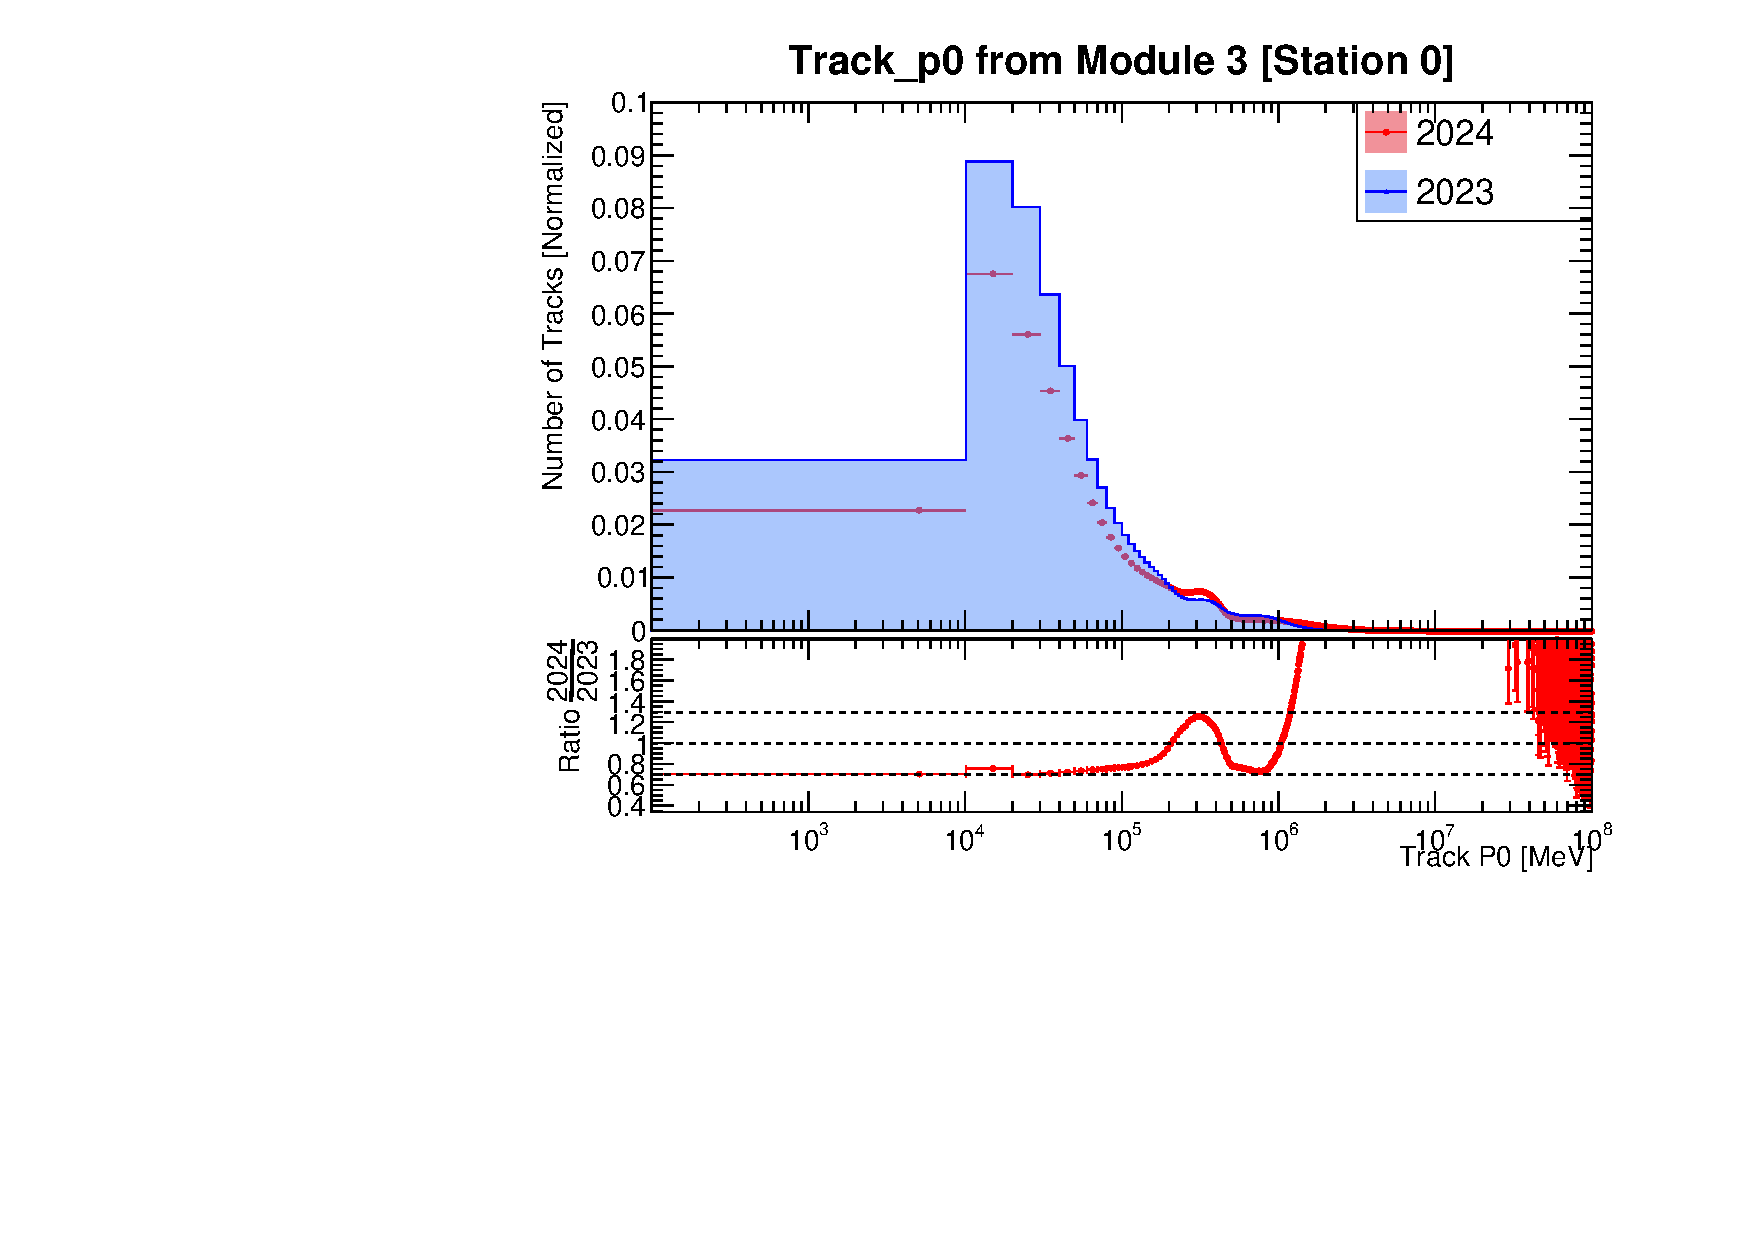
\includegraphics[width=\linewidth]{./ModuleLevelPlots/Track_p0_st0_module3_linear.pdf}
%         \end{subfigure}
%         \begin{subfigure}[t]{0.49\linewidth}
%             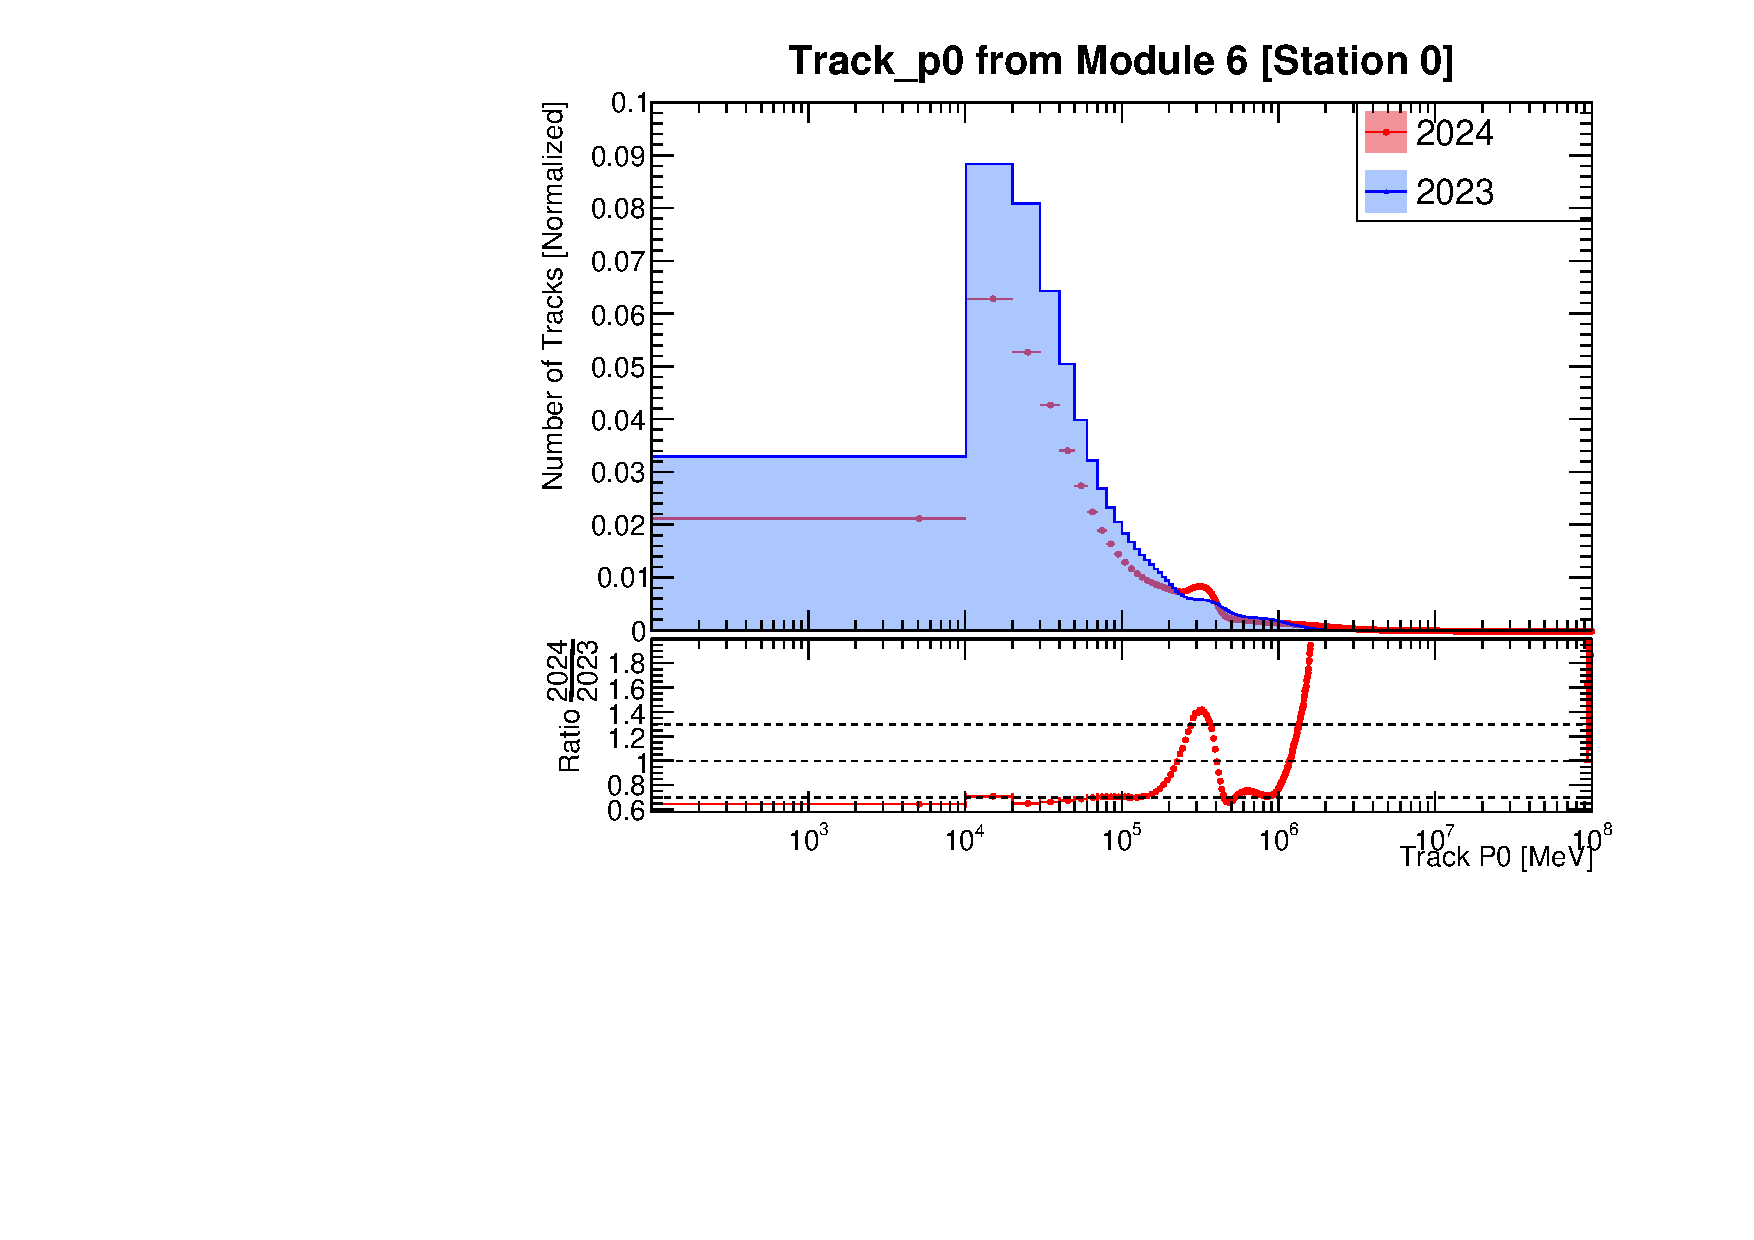
\includegraphics[width=\linewidth]{./ModuleLevelPlots/Track_p0_st0_module6_linear.pdf}
%         \end{subfigure}

%         \begin{subfigure}[t]{0.49\linewidth}
%             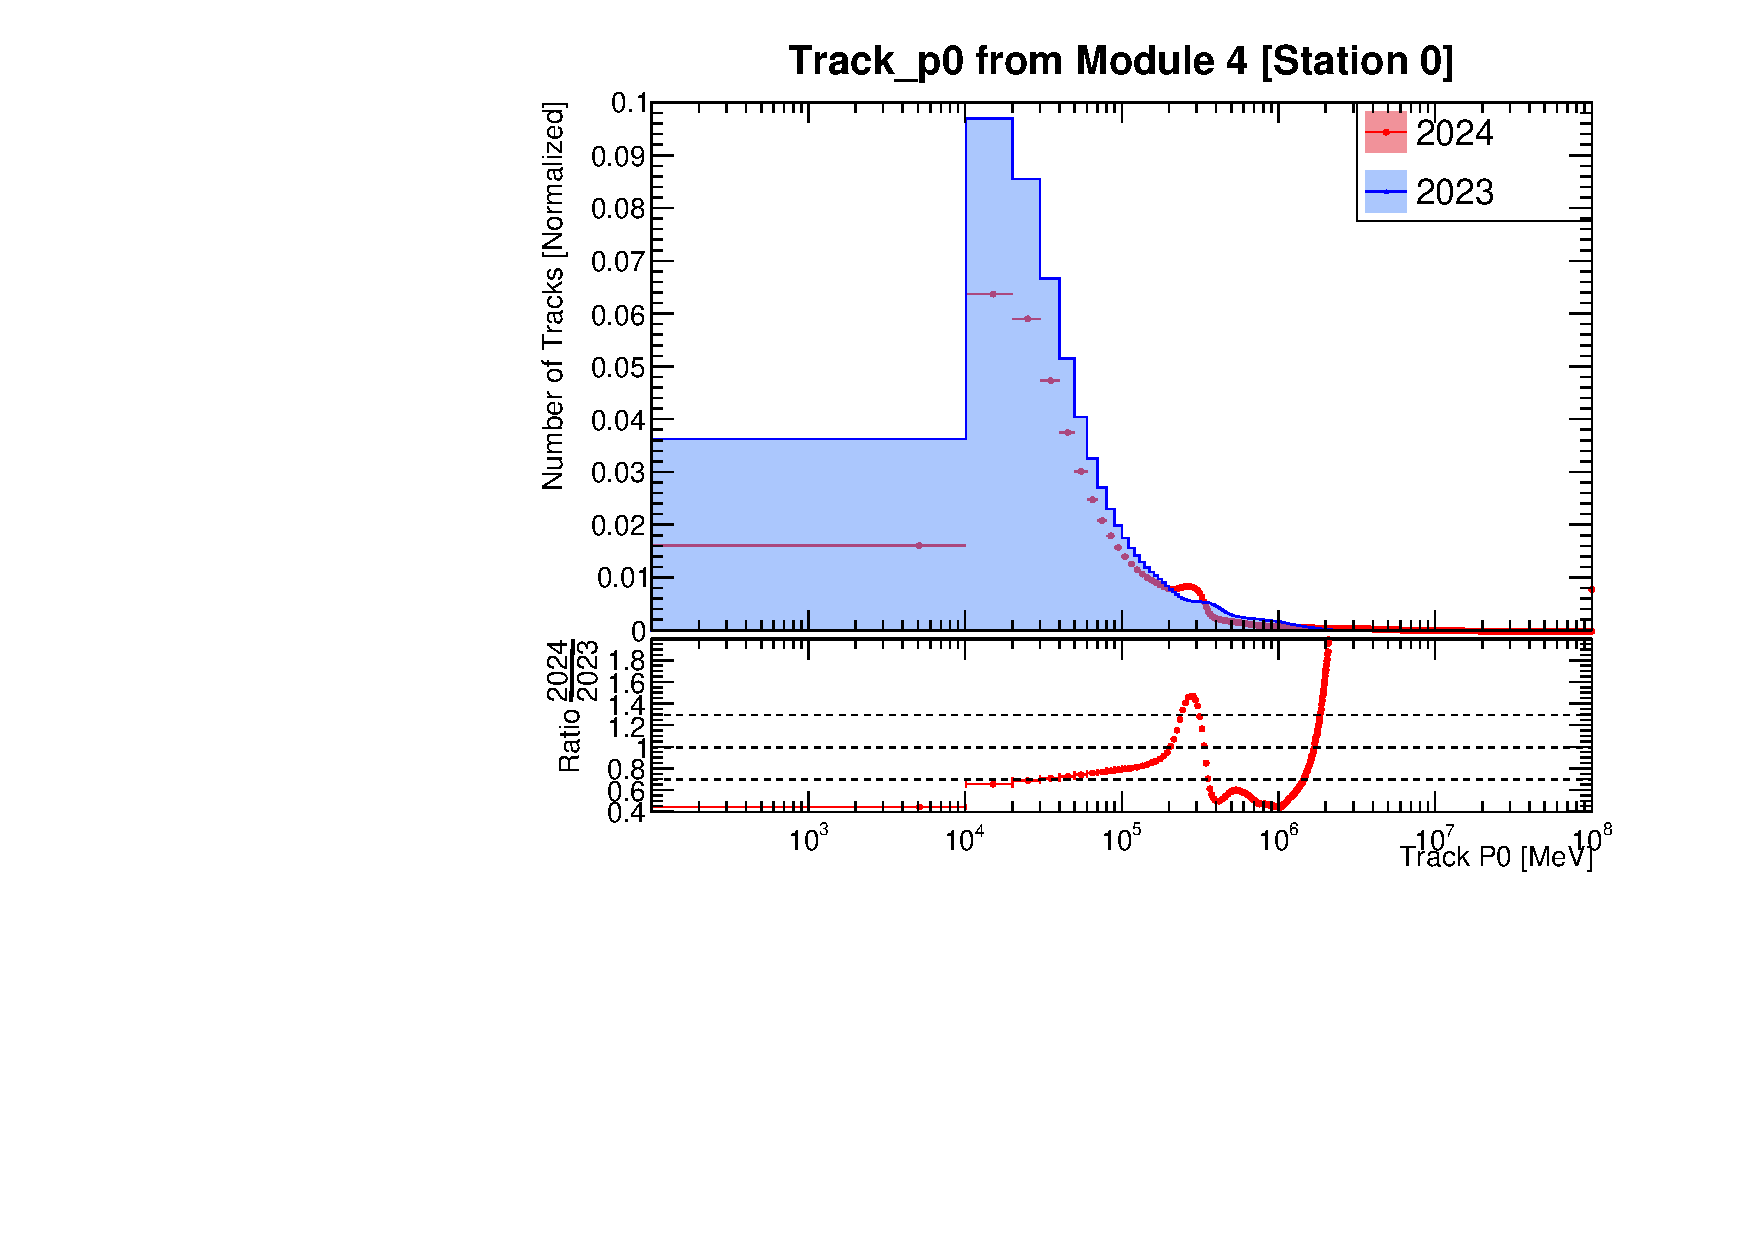
\includegraphics[width=\linewidth]{./ModuleLevelPlots/Track_p0_st0_module4_linear.pdf}
%         \end{subfigure}
%         \begin{subfigure}[t]{0.49\linewidth}
%             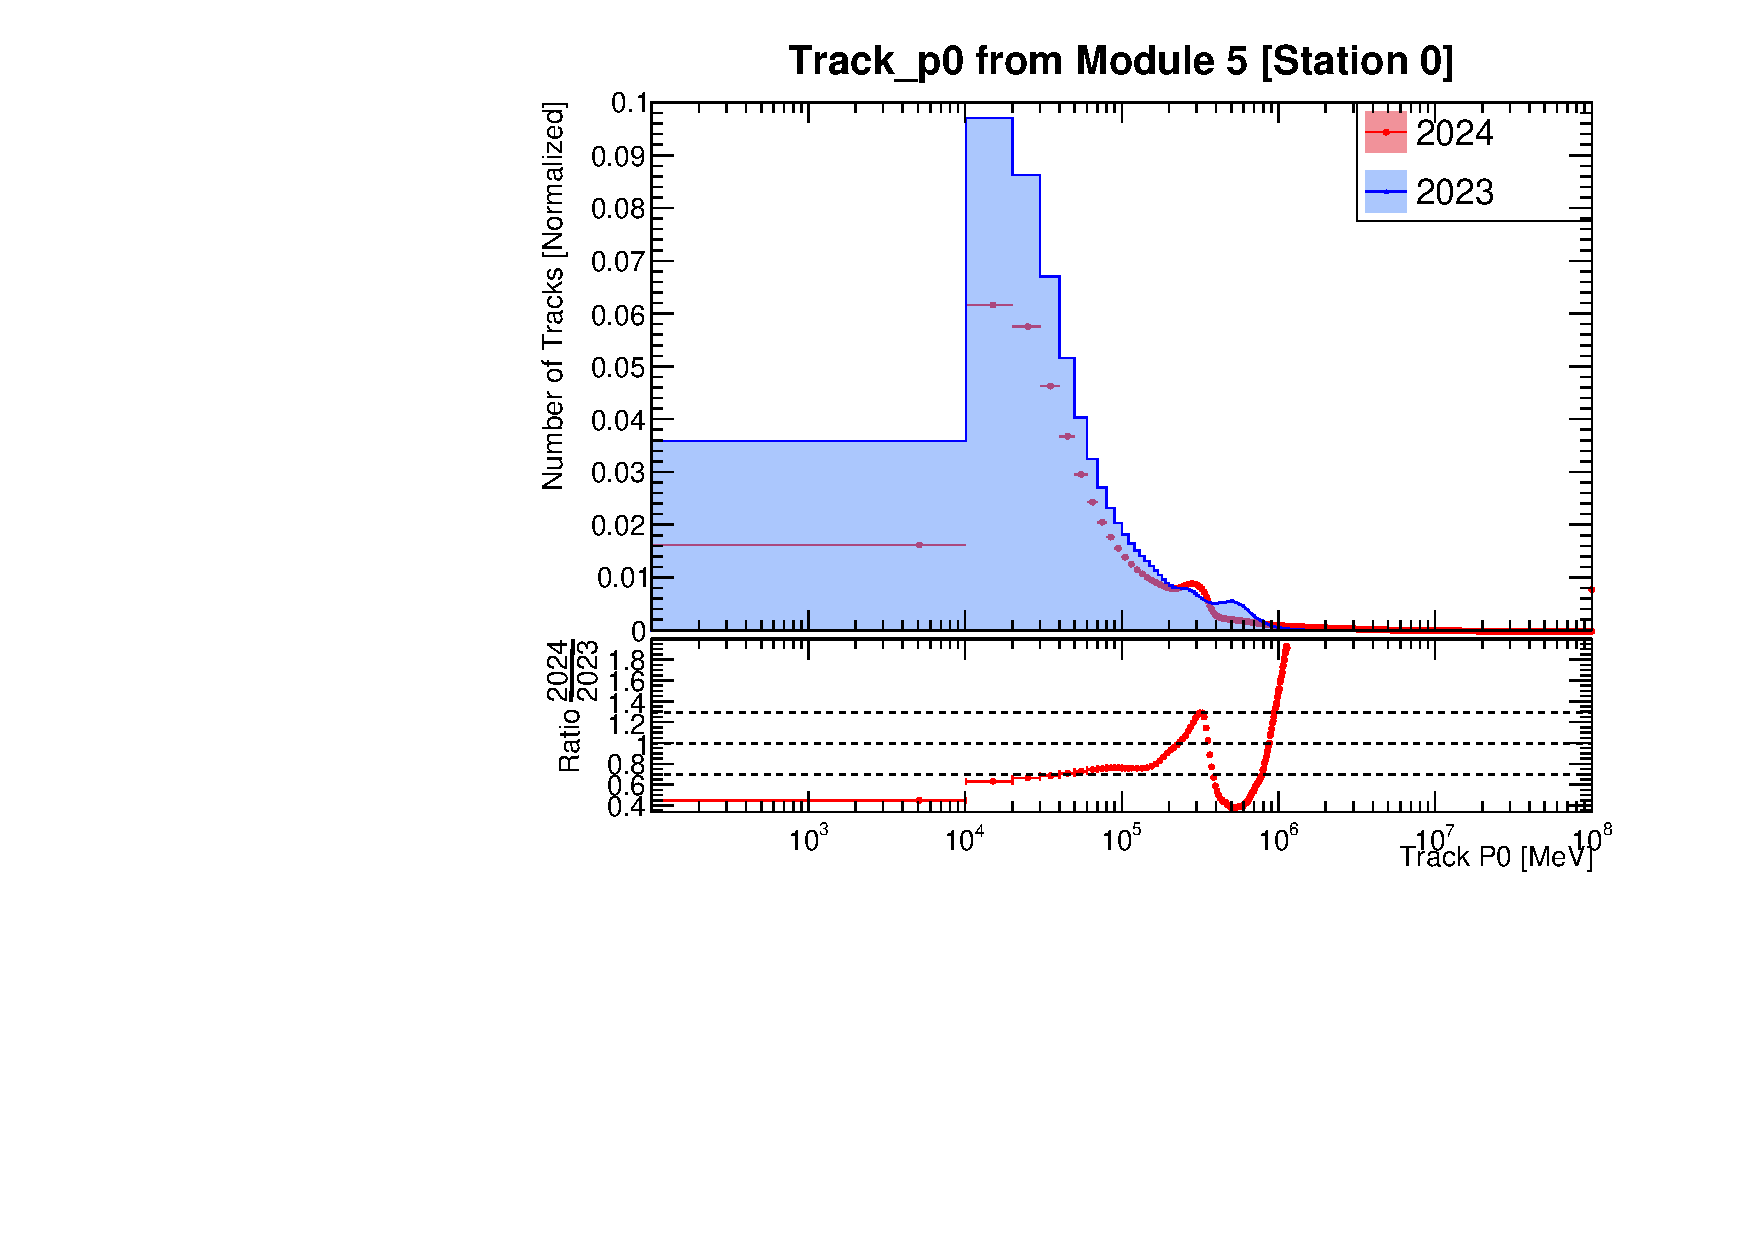
\includegraphics[width=\linewidth]{./ModuleLevelPlots/Track_p0_st0_module5_linear.pdf}
%         \end{subfigure}
%     \end{figure}
% \end{frame}

\begin{frame}{Distribution of Track Momenta Modulewise}
    \begin{columns}
        \begin{column}{0.6\linewidth}
            \begin{figure}
                \centering
                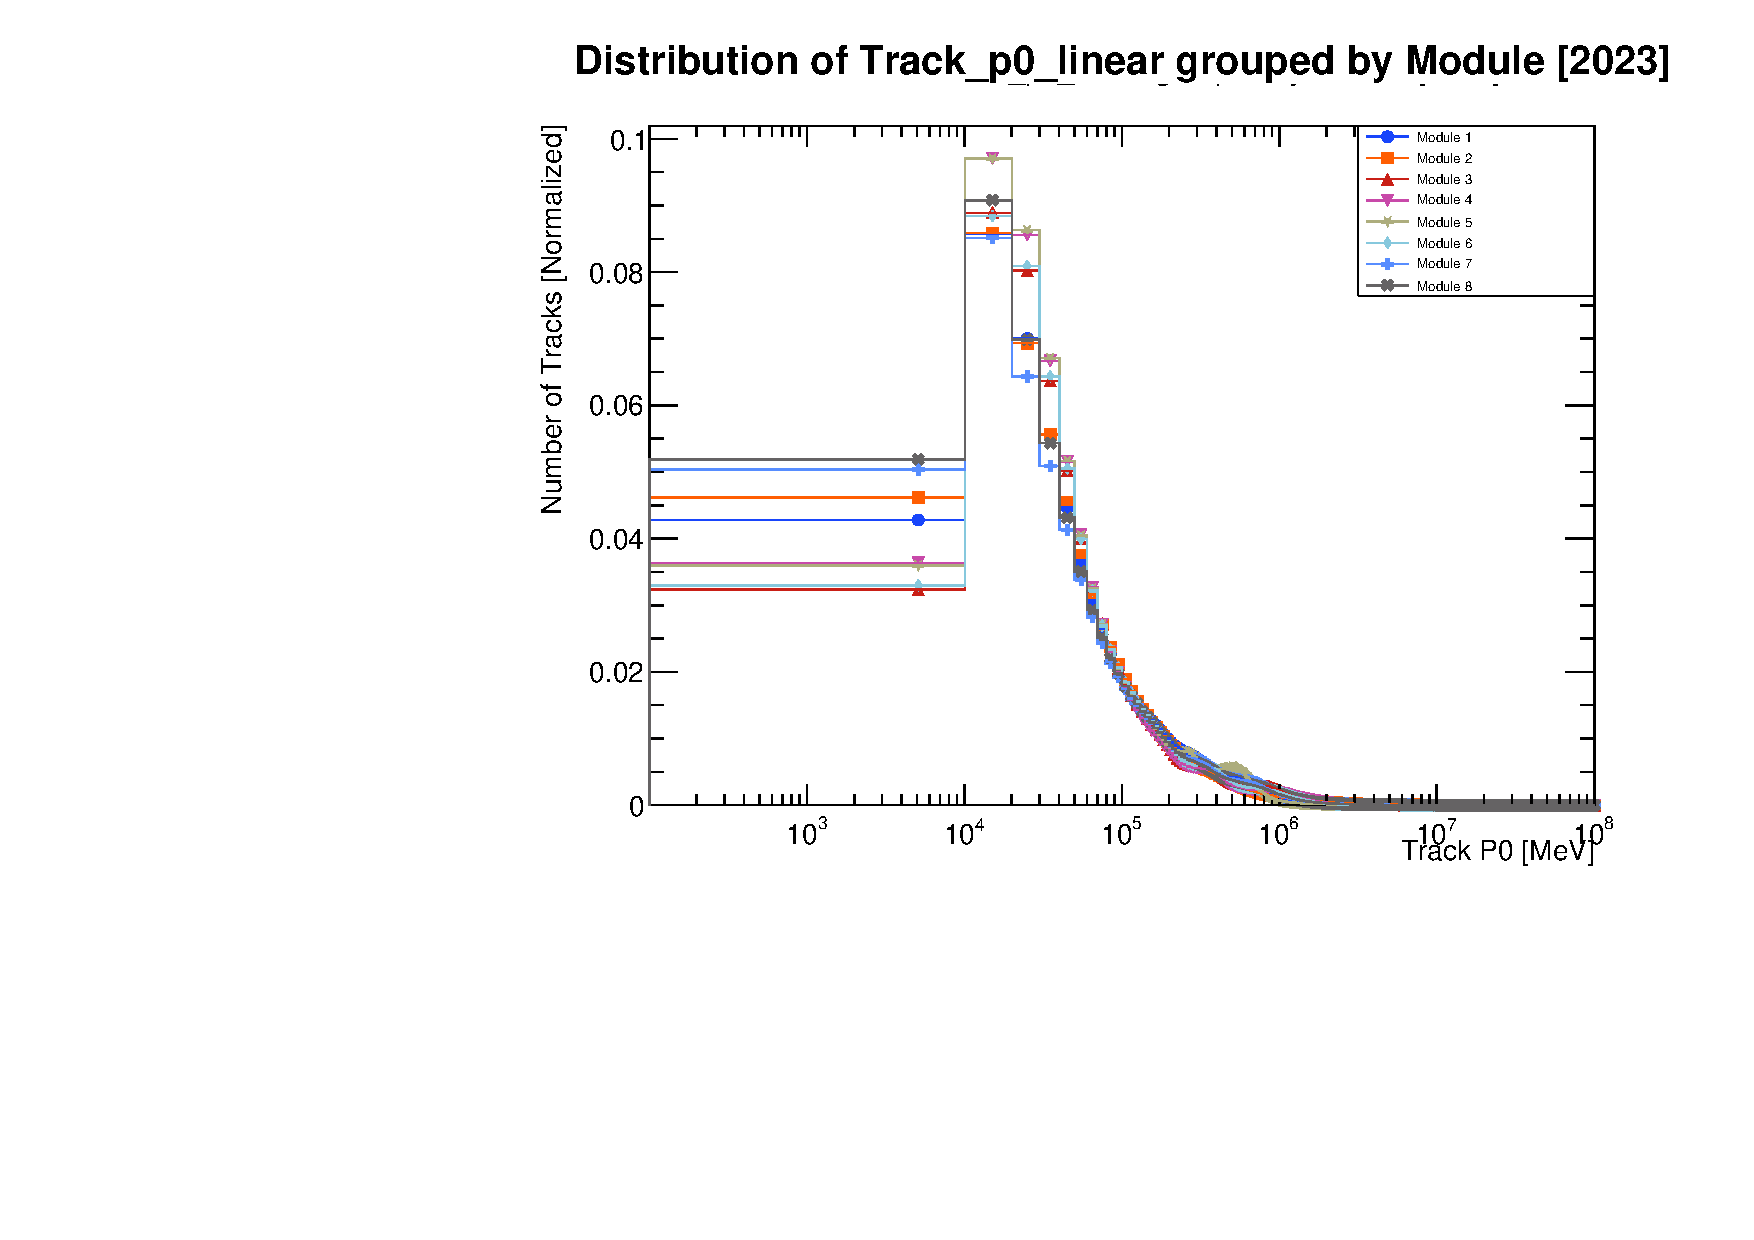
\includegraphics[width=\linewidth]{./ModuleLevelPlots/Track_p0_linear_st0_2023.pdf}
            \end{figure}
        \end{column}
        \begin{column}{0.6\linewidth}
            \begin{figure}
                \centering
                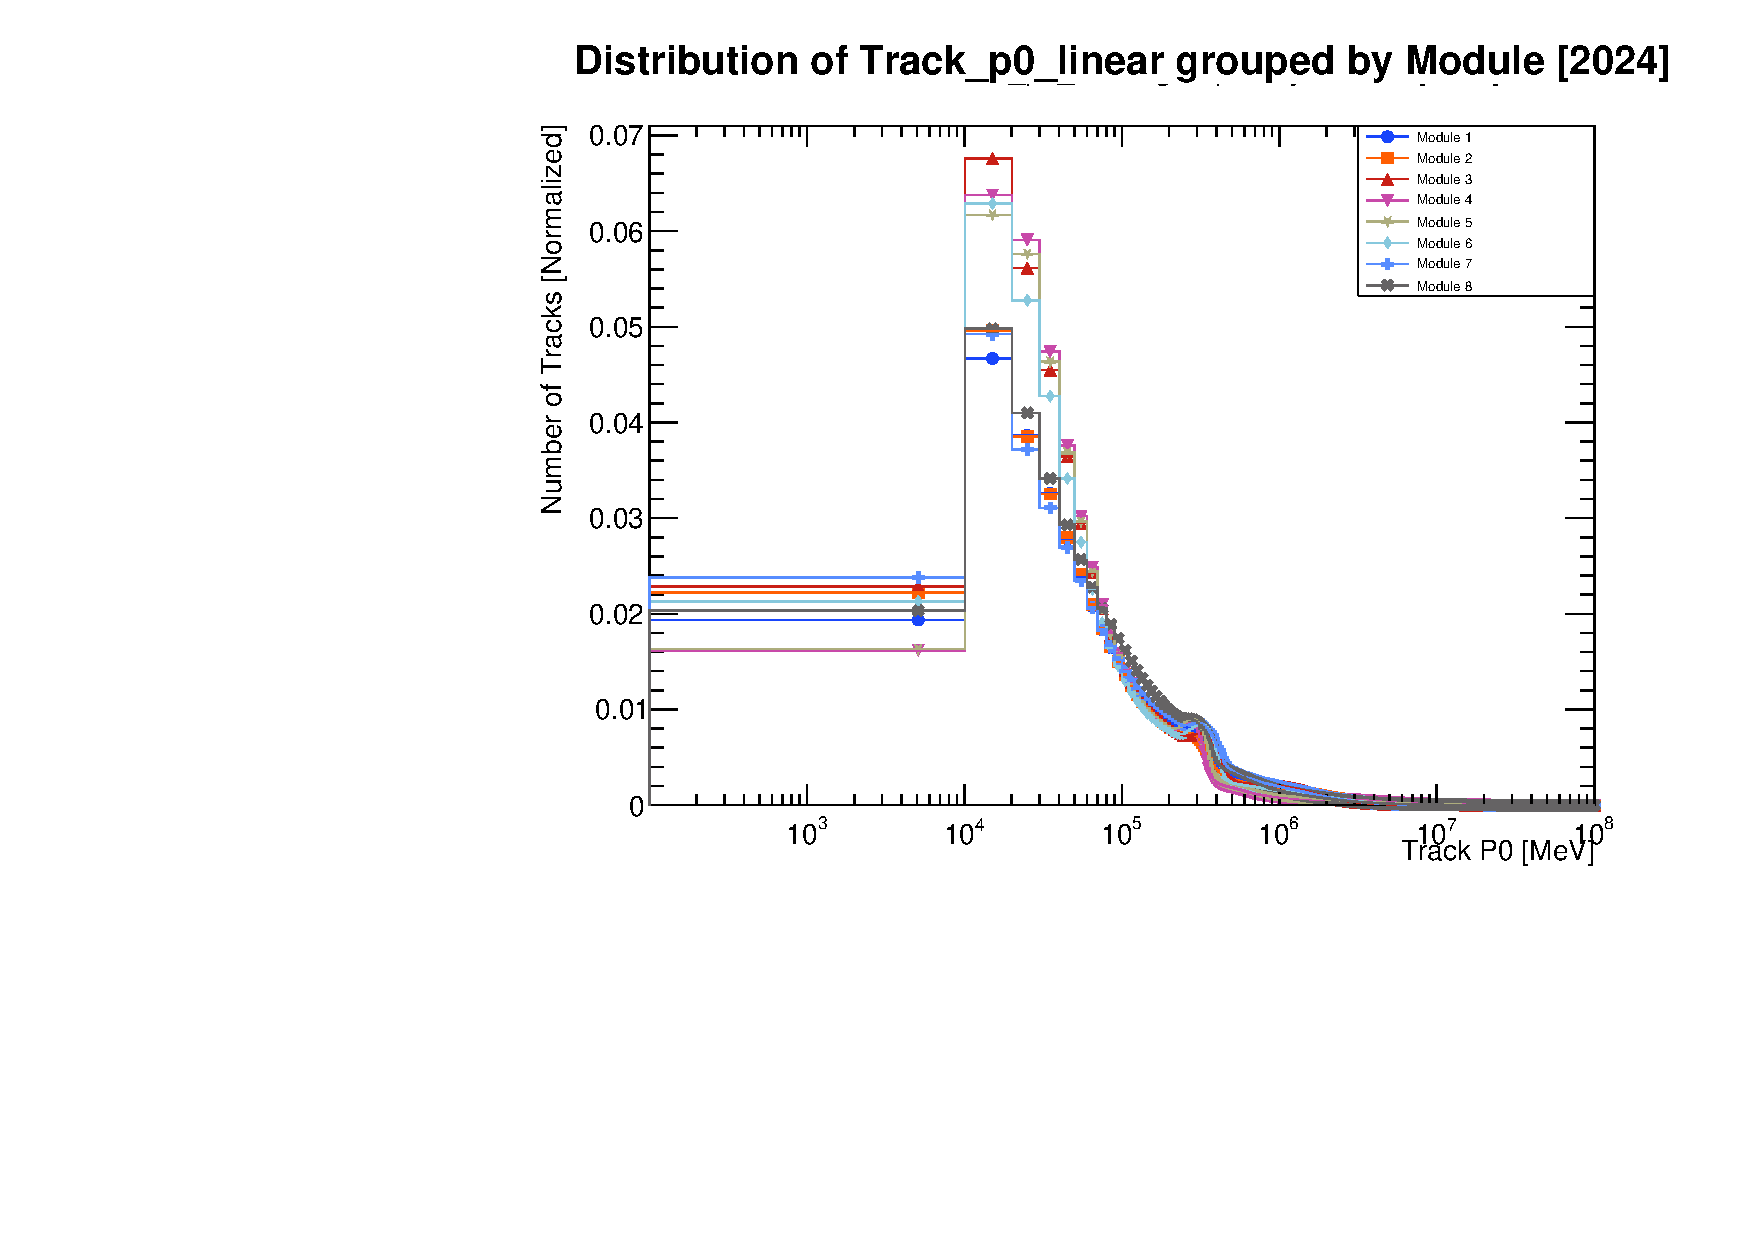
\includegraphics[width=\linewidth]{./ModuleLevelPlots/Track_p0_linear_st0_2024.pdf}
            \end{figure}
        \end{column}
    \end{columns}

    \begin{itemize}
        \small
        \item Distribution different across modules and years 
        \item Leading to lack of agreement in other parameters
        \item Modules tend to group together
        \begin{itemize}
            \item Higher Momenta Modules : 3, 4, 5, 6  [Modules with y $\leq$ 0]
            \item Lower Momenta Modules \ : 2, 1, 8, 7 [Modules with y $\geq$ 0]
        \end{itemize}
    \end{itemize}
\end{frame}

% \makemodulewiseframes{Track_charge}{Distribution of Track Charge Modulewise}
\begin{frame}{Distribution Track Charge Modulewise}
    \newcommand{\colname}{Track_charge}
    \begin{columns}
        \begin{column}{0.6\linewidth}
            \begin{figure}
                \centering
                \includegraphics[width=\linewidth]{./ModuleLevelPlots/\colname_st0_2023.pdf}
            \end{figure}
        \end{column}
        \begin{column}{0.6\linewidth}
            \begin{figure}
                \centering
                \includegraphics[width=\linewidth]{./ModuleLevelPlots/\colname_st0_2024.pdf}
            \end{figure}
        \end{column}
    \end{columns}

    \begin{itemize}
        \small
        \item Track Charge distribution is different across modules and years
        \item 2024 has more positively charged tracks than 2023 
        \item In 2023 Module 1,2 seem to get more positively charged tracks
        \item In 2024 Module 3,6,7,5 seem to get more positively charged tracks
        % \begin{itemize}
        %     \item Suggests, positive tracks concentrated in the bottom right?
        % \end{itemize}
    \end{itemize}
\end{frame}
% \begin{frame}{Summary of Module Level Analysis}
    
% \end{frame}
\begin{frame}{Runwise Analysis of 2024 Data}
    \begin{itemize}
        \item In 2024, FaserNu had to be replaced every 10 fb$^{-1}$.
        \item The replacement schedule was as follows
    \end{itemize}
    \begin{table}[h!]
        \begin{tabular}{|l|c|c|c|}
            \hline
            \textbf{Box}  & \textbf{Installed} & \textbf{Removed} & \textbf{Lumi (ifb)} \\ \hline
            F241          & 20/3               & 6/5              & 11.6                \\ \hline
            Tungsten only & 6/5                & 12/6             & 18.5                \\ \hline
            F242          & 12/6               & 8/7              & 9.9                 \\ \hline
            CaloNu        & 10/7               & 4/10             & 69.8                \\ \hline
            F243          & 4/10               & 22/10            & 11.9                \\ \hline
        \end{tabular}
		\vspace{0.3cm}
        \caption{Replacement Schedule [Source: \href{https://indico.cern.ch/event/1350805/contributions/5686417/attachments/2963344/5212652/FASER-GeneralMtg-8.11.24.pdf}{FASER General Meeting 8.11.24}]}
    \end{table}
	\vspace{-0.5cm}
    \begin{itemize}
        \item The runs are split into categories based on the above schedule
        \item We can look at the Yield for each category, 
		\begin{itemize}
			\item NEvents/Lumi : Top Plot
			\item  NTracks/Lumi : Botton Plot
		\end{itemize}
    \end{itemize}
    \tiny{Note: Detailed Calculation of Run Numbers and Problematic Yields can be found here \href{https://docs.google.com/spreadsheets/d/1nnYFcmhVieSHI5XAVhPiW1K6CoGYGxv2YPchwL0sqH4/edit?usp=sharing}{[Link to Sheet]}}
\end{frame}

\begin{frame}{Issues with BCID}
	\begin{itemize}
		\item Reminder that the 2024 data is split into as p0011 and p0012
		\item The p0011 data has issues with the BCID makes the distanceToCollidingBCID unreliable
		\item But unfortunately, p0011 data is more than 55\% of the 2024 data thus cannot be ignored.
		\item Following plots apply the BCID cut only on the 2023 data and the p0012 data, the first 55 runs do not pass the cut at all.
	\end{itemize}
	\begin{figure}
		\includegraphics[width=\linewidth]{./assets/BCIDEfficiency_p0011.pdf}
		\caption{Efficiency of the BCID cut on the p0011 data}
	\end{figure}

\end{frame}

\begin{frame}{Yield Plots for F241-2024}
	\begin{center}
		\begin{tikzpicture}
			\node[anchor=south west, inner sep=0] (image) at (0,0) {\includegraphics[height=0.4\textheight]{RunwisePlots/F241-2024_NEventsbyLumi.pdf}};
			\begin{scope}[x={(image.south east)},y={(image.north west)}]
				% \draw[help lines,xstep=.1,ystep=.1] (0,0) grid (1,1);
				\draw[red] (0.06,0.6) rectangle (0.25,0.84);
				\node[red, below, scale=0.6] at (0.155,0.6) {\tiny Early Runs Erratic};
				\draw[red] (0.455,0.69) rectangle (0.475,0.73);
				\node[red, right, scale=0.6] at (0.48,0.71) {\tiny Potentially Problematic [14776]};
			\end{scope}
		\end{tikzpicture}
	\end{center}
	\begin{center}
	\begin{tikzpicture}
		\centering
		\node[anchor=south west, inner sep=0] (image) at (0,0) {\includegraphics[height=0.4\textheight]{RunwisePlots/F241-2024_NTracksbyLumi.pdf}};
		\begin{scope}[x={(image.south east)},y={(image.north west)}]
			% \draw[help lines,xstep=.1,ystep=.1] (0,0) grid (1,1);
			\draw[red] (0.06,0.35) rectangle (0.25,0.4);
			\node[red, below, scale=0.6] at (0.155,0.36) {\tiny Less Pronounced!};
			\draw[red] (0.455,0.37) rectangle (0.475,0.4);
			% \node[red, right, scale=0.6] at (0.48,0.39) {\tiny Potentially Problematic [14776]};
		\end{scope}
	\end{tikzpicture}
\end{center}

\end{frame}

\begin{frame}{Yield Plots for Tungsten-2024}
	\begin{center}
	\begin{tikzpicture}
		\node[anchor=south west, inner sep=0] (image) at (0,0) {\includegraphics[height=0.4\textheight]{RunwisePlots/Tungsten-2024_NEventsbyLumi.pdf}};
		\begin{scope}[x={(image.south east)},y={(image.north west)}]
			% \draw[help lines,xstep=.1,ystep=.1] (0,0) grid (1,1);
			\draw[red] (0.065,0.198) rectangle (0.17,0.22);
			\node[red, above, scale=0.6] at (0.12,0.24) {\tiny Early Runs High?};
			\draw[red] (0.22,0.2) rectangle (0.37,0.93);
			\node[red, right, scale=0.6] at (0.37,0.6) {\tiny Unusually High! Throws off the scale};
			% \draw[red] (0.455,0.69) rectangle (0.475,0.73);
			% \node[red, right, scale=0.6] at (0.48,0.71) {\tiny Potentially Problematic [14776]};
		\end{scope}
	\end{tikzpicture}
	\end{center}
	\begin{center}
	\begin{tikzpicture}
		\node[anchor=south west, inner sep=0] (image) at (0,0) {\includegraphics[height=0.4\textheight]{RunwisePlots/Tungsten-2024_NTracksbyLumi.pdf}};
		\begin{scope}[x={(image.south east)},y={(image.north west)}]
			% \draw[help lines,xstep=.1,ystep=.1] (0,0) grid (1,1);
			\draw[red] (0.062,0.335) rectangle (0.165,0.36);
			\node[red, above, scale=0.6] at (0.12,0.36) {\tiny Seem better here?};
			\draw[red] (0.22,0.45) rectangle (0.37,0.93);
			\node[red, right, scale=0.6] at (0.37,0.65) {\tiny Unusual!};
			\draw[red] (0.64,0.35) rectangle (0.8,0.4);
			\draw[red] (0.95,0.35) rectangle (0.99,0.4);
			\draw[red] (0.8,0.4) -- (0.95,0.4);
			\node[red, right, scale=0.6] at (0.83,0.43) {\tiny Slightly Elevated?};
		\end{scope}
	\end{tikzpicture}
\end{center}
\end{frame}

\begin{frame}{Yield Plots for F242-2024}
\begin{center}
	\begin{tikzpicture}
		\node[anchor=south west, inner sep=0] (image) at (0,0) {\includegraphics[height=0.4\textheight]{RunwisePlots/F242-2024_NEventsbyLumi.pdf}};
		\begin{scope}[x={(image.south east)},y={(image.north west)}]
			% \draw[help lines,xstep=.1,ystep=.1] (0,0) grid (1,1);
			\draw[red] (0.06,0.8) rectangle (0.08,0.9);
			\node[red, right, scale=0.6] at (0.08,0.85) {\tiny High};
			\draw[red] (0.335,0.76) rectangle (0.35,0.82);
			\node[red, right, scale=0.6] at (0.35,0.80) {\tiny  High};
			\draw[red] (0.215,0.32) rectangle (0.23,0.355);
			\node[red, below, scale=0.6] at (0.225,0.34) {\tiny  Low?};
			\draw[red] (0.879,0.275) rectangle (0.89,0.31);
			\node[red, below, scale=0.6] at (0.885,0.275) {\tiny  Low};
		\end{scope}
	\end{tikzpicture}
\end{center}
\begin{center}
	\begin{tikzpicture}
		\node[anchor=south west, inner sep=0] (image) at (0,0) {\includegraphics[height=0.4\textheight]{RunwisePlots/F242-2024_NTracksbyLumi.pdf}};
		\begin{scope}[x={(image.south east)},y={(image.north west)}]
			% \draw[help lines,xstep=.1,ystep=.1] (0,0) grid (1,1);
			\draw[red] (0.06,0.34) rectangle (0.2,0.4);
			\node[red, above, scale=0.6] at (0.13,0.4) {\tiny Slightly Elevated};
			\draw[red] (0.335,0.65) rectangle (0.35,0.7);
			\node[red, above, scale=0.6] at (0.3425,0.7) {\tiny  High};
			\draw[red] (0.215,0.32) rectangle (0.23,0.355);
			\node[red, below, scale=0.6] at (0.225,0.34) {\tiny  Low?};
			\draw[red] (0.879,0.275) rectangle (0.89,0.31);
			\node[red, below, scale=0.6] at (0.885,0.275) {\tiny  Low};
		\end{scope}
	\end{tikzpicture}
\end{center}

\end{frame}

\begin{frame}{Yield Plots for CaloNu-2024}
\begin{center}
	\begin{tikzpicture}
		\node[anchor=south west, inner sep=0] (image) at (0,0) {\includegraphics[height=0.4\textheight]{RunwisePlots/CaloNu-2024_NEventsbyLumi.pdf}};
		\begin{scope}[x={(image.south east)},y={(image.north west)}]
			% \draw[help lines,xstep=.05,ystep=.05] (0,0) grid (1,1);
			% \foreach \x in {0,1,...,9} { \node [anchor=north] at (\x/10,0) {0.\x}; }
			% \foreach \y in {0,1,...,9} { \node [anchor=east] at (0,\y/10) {0.\y}; }
			\draw[red] (0.78,0.71) rectangle (0.81,0.76);
			\node[red, above, scale=0.6] at (0.795,0.76) {\tiny High};
			\draw[red] (0.335,0.41) rectangle (0.35,0.45);
			\node[red, above, scale=0.6] at (0.3425,0.45) {\tiny High?};
			\draw[red] (0.215,0.35) rectangle (0.225,0.375);
			\draw[red] (0.595,0.35) rectangle (0.61,0.38);
			\draw[red] (0.639,0.358) rectangle (0.655,0.385);
			\draw[red] (0.675,0.35) rectangle (0.683,0.373);
			\draw[red] (0.872,0.36) rectangle (0.88,0.38);
			\draw[red] (0.445,0.17) rectangle (0.46,0.2);
			\node[red, above, scale=0.6] at (0.495, 0.19) {\tiny Low};
			\draw[red] (0.525,0.2) rectangle (0.54,0.22);
			\draw[red] (0.965,0.16) rectangle (0.975,0.19);
			\node[red, above, scale=0.6] at (0.97,0.19) {\tiny Low};
		\end{scope}
	\end{tikzpicture}
\end{center}
\begin{center}
	\begin{tikzpicture}
		\node[anchor=south west, inner sep=0] (image) at (0,0) {\includegraphics[height=0.4\textheight]{RunwisePlots/CaloNu-2024_NTracksbyLumi.pdf}};
		\begin{scope}[x={(image.south east)},y={(image.north west)}]
			\draw[red] (0.78,0.71) rectangle (0.81,0.76);
			\node[red, above, scale=0.6] at (0.795,0.76) {\tiny High};
			\draw[red] (0.3375,0.39) rectangle (0.35,0.41);
			\node[red, above, scale=0.6] at (0.3475,0.41) {\tiny Better?};
			\draw[red] (0.215,0.35) rectangle (0.225,0.375);
			\draw[red] (0.595,0.35) rectangle (0.61,0.38);
			\draw[red] (0.639,0.358) rectangle (0.655,0.385);
			\draw[red] (0.675,0.35) rectangle (0.683,0.373);
			\draw[red] (0.872,0.36) rectangle (0.88,0.38);
			\draw[red] (0.445,0.17) rectangle (0.46,0.2);
			\node[red, above, scale=0.6] at (0.495, 0.19) {\tiny Low};
			\draw[red] (0.525,0.2) rectangle (0.54,0.22);
			\draw[red] (0.965,0.16) rectangle (0.975,0.19);
			\node[red, above, scale=0.6] at (0.97,0.19) {\tiny Low};
		\end{scope}
	\end{tikzpicture}
\end{center}
\end{frame}

\begin{frame}{Yield Plots for F243-2024}
	\begin{center}
	\begin{tikzpicture}
		\node[anchor=south west, inner sep=0] (image) at (0,0) {\includegraphics[height=0.4\textheight]{RunwisePlots/F243-2024_NEventsbyLumi.pdf}};
		\begin{scope}[x={(image.south east)},y={(image.north west)}]
			% \draw[help lines,xstep=.1,ystep=.1] (0,0) grid (1,1);
			\draw[red] (0.15,0.29) rectangle (0.165,0.33);
			\draw[red] (0.19,0.15) rectangle (0.205,0.17);
			\node[red, above, scale=0.6] at (0.1975,0.16) {\tiny Zero!};
			\draw[red] (0.515,0.15) rectangle (0.53,0.17);
			\draw[red] (0.598,0.15) rectangle (0.61,0.17);
			\node[red, above, scale=0.6] at (0.564,0.15) {\tiny Zero!};
			\draw[red] (0.64,0.2) rectangle (0.65,0.25);
			\draw[red] (0.76,0.18) rectangle (0.773,0.22);
			\draw[red] (0.84,0.28) rectangle (0.854,0.3);
			\draw[red] (0.925,0.205) rectangle (0.935,0.23);
		\end{scope}
	\end{tikzpicture}
\end{center}
	\begin{center}
	\begin{tikzpicture}
		\node[anchor=south west, inner sep=0] (image) at (0,0) {\includegraphics[height=0.4\textheight]{RunwisePlots/F243-2024_NTracksbyLumi.pdf}};
		\begin{scope}[x={(image.south east)},y={(image.north west)}]
			% \draw[help lines,xstep=.1,ystep=.1] (0,0) grid (1,1);
			\draw[red] (0.15,0.29) rectangle (0.165,0.33);
			\draw[red] (0.19,0.15) rectangle (0.205,0.17);
			\node[red, above, scale=0.6] at (0.1975,0.16) {\tiny Zero!};
			\draw[red] (0.515,0.15) rectangle (0.53,0.17);
			\draw[red] (0.598,0.15) rectangle (0.61,0.17);
			\node[red, above, scale=0.6] at (0.564,0.15) {\tiny Zero!};
			\draw[red] (0.64,0.2) rectangle (0.65,0.25);
			\draw[red] (0.76,0.18) rectangle (0.773,0.22);
			\draw[red] (0.84,0.28) rectangle (0.854,0.3);
			\draw[red] (0.925,0.205) rectangle (0.935,0.23);
		\end{scope}
	\end{tikzpicture}
	\end{center}
\end{frame}



% \begin{frame}{Yield Plots for F241-2024}
% 	\begin{figure}
% 		\includegraphics[height=0.4\textheight]{RunwisePlots/F241-2024_NEventsbyLumi.pdf}
% 	\end{figure}
% 	\begin{figure}
% 		\includegraphics[height=0.4\textheight]{RunwisePlots/F241-2024_NTracksbyLumi.pdf}
% 	\end{figure}
% \end{frame}

% \begin{frame}{Yield Plots for Tungsten-2024}
% 	\begin{figure}
% 		\includegraphics[height=0.4\textheight]{RunwisePlots/Tungsten-2024_NEventsbyLumi.pdf}
% 	\end{figure}
% 	\begin{figure}
% 		\includegraphics[height=0.4\textheight]{RunwisePlots/Tungsten-2024_NTracksbyLumi.pdf}
% 	\end{figure}
% \end{frame}

% \begin{frame}{Yield Plots for F242-2024}
% 	\begin{figure}
% 		\includegraphics[height=0.4\textheight]{RunwisePlots/F242-2024_NEventsbyLumi.pdf}
% 	\end{figure}
% 	\begin{figure}
% 		\includegraphics[height=0.4\textheight]{RunwisePlots/F242-2024_NTracksbyLumi.pdf}
% 	\end{figure}
% \end{frame}

% \begin{frame}{Yield Plots for CaloNu-2024}
% 	\begin{figure}
% 		\includegraphics[height=0.4\textheight]{RunwisePlots/CaloNu-2024_NEventsbyLumi.pdf}
% 	\end{figure}
% 	\begin{figure}
% 		\includegraphics[height=0.4\textheight]{RunwisePlots/CaloNu-2024_NTracksbyLumi.pdf}
% 	\end{figure}
% \end{frame}

% \begin{frame}{Yield Plots for F243-2024}
% 	\begin{figure}
% 		\includegraphics[height=0.4\textheight]{RunwisePlots/F243-2024_NEventsbyLumi.pdf}
% 	\end{figure}
% 	\begin{figure}
% 		\includegraphics[height=0.4\textheight]{RunwisePlots/F243-2024_NTracksbyLumi.pdf}
% 	\end{figure}
% \end{frame}

\begin{frame}{Median Yields across Runs}
	\begin{figure}
		\includegraphics[width=\linewidth]{./RunwisePlots/MedianYieldsPhase.pdf}
	\end{figure}
	\vspace{-0.5cm}
	\begin{itemize}
		\item Possible anomaly in the F241 data from lack of BCID cut.
		\item Detailed Listing of runs with problematic yields. \href{https://docs.google.com/spreadsheets/d/1nnYFcmhVieSHI5XAVhPiW1K6CoGYGxv2YPchwL0sqH4/edit?usp=sharing}{[LINK]}
	\end{itemize}
\end{frame}

% \begin{frame}{Distribution of Track Parameters across Runs}
% 	\begin{center}
% 		Excellent agreement of variables across runs !
% 	\end{center}
	
% \end{frame}


\begin{frame}{Distribution of Track Position/Angle across runs}
	\begin{columns}
		\begin{column}{0.5\linewidth}
			\vspace{-0.4cm}
			\begin{figure}
				\includegraphics[width=\linewidth]{./RunwisePlots/Track_x0_runwise.pdf}
				\caption{Distribution of Track Position X0}
			\end{figure}
			\vspace{-0.9cm}
			\begin{figure}
				\includegraphics[width=\linewidth]{./RunwisePlots/Track_ThetaX_0_runwise.pdf}
				\caption{Distribution of Track ThetaX0 across 2024 runs}
			\end{figure}
		\end{column}
		\begin{column}{0.5 \linewidth}
			\vspace{-0.4cm}
			\begin{figure}
				\includegraphics[width=\linewidth]{./RunwisePlots/Track_y0_runwise.pdf}
				\caption{Distribution of Track Position in Y0}
			\end{figure}
			\vspace{-0.9cm}
			\begin{figure}
				\includegraphics[width=\linewidth]{./RunwisePlots/Track_ThetaY_0_runwise.pdf}
				\caption{Distribution of Track ThetaY0 across 2024 runs}
			\end{figure}
		\end{column}
	\end{columns}
	% \begin{itemize}
	% 	\item General, run-wise agreement is excellent for the Track variables
	% \end{itemize}
\end{frame}


% \begin{frame}{Distribution of Track Angles across 2024 runs}
% 	\begin{columns}
% 		\begin{column}{0.5\linewidth}
% 			\begin{figure}
% 				\includegraphics[width=\linewidth]{./RunwisePlots/Track_ThetaX_0_runwise.pdf}
% 				\caption{Distribution of Track ThetaX0 across 2024 runs}
% 			\end{figure}
% 		\end{column}
% 		\begin{column}{0.5 \linewidth}
% 			\begin{figure}
% 				\includegraphics[width=\linewidth]{./RunwisePlots/Track_ThetaY_0_runwise.pdf}
% 				\caption{Distribution of Track ThetaY0 across 2024 runs}
% 			\end{figure}
% 		\end{column}	
% 	\end{columns}
% \end{frame}


\begin{frame}{Distribution of Track Momenta/Charge across runs}
	\begin{columns}
		\begin{column}{0.5\linewidth}
			\begin{figure}
				\includegraphics[width=\linewidth]{./RunwisePlots/Track_p0_runwise.pdf}
				\caption{Distribution of Track Momenta in MeV across 2024 runs, as measured by the first tracking station}
			\end{figure}
		\end{column}
		\begin{column}{0.5\linewidth}
			\begin{figure}
				\includegraphics[width=\linewidth]{./RunwisePlots/Track_charge_runwise.pdf}
				\caption{Distribution of Track Charge across 2024 runs}
			\end{figure}
		\end{column}
	\end{columns}
	\begin{itemize}
		\item The background seems consistent across the runs as well.
		\item Really good agreement across runs for all tracking parameters (Track $\chi^{2}$ etc) across the five 2024 run periods.
	\end{itemize}
\end{frame}

\begin{frame}{Distribution of longTracks across 2024 runs}
	\begin{columns}
		\begin{column}{0.55 \linewidth}
			\begin{figure}
				\includegraphics[width=\linewidth]{./RunwisePlots/longTracks_runwise.pdf}
				\caption{LongTracks across 2024 runs [Normalized to Sum of Entries across all bins]}
			\end{figure}
		\end{column}
		\begin{column}{0.55 \linewidth}
			\begin{figure}
				\includegraphics[width=\linewidth]{RunwisePlots/longTracks_normalisedfrom2_runwise.pdf}
				\caption{LongTracks across 2024 runs [Normalized to Sum of Entries starting from 2nd bin]}
			\end{figure}
		\end{column}
	\end{columns}
	\begin{itemize}
		\item F241 seems to show a higher number of 0-longTrack events.
		\item Most likely from the lack of BCID cut for the early runs (less bunches) in F241.
	\end{itemize}
	% \begin{figure}
	% 	\begin{subfigure}{0.45\linewidth}
	% 		\includegraphics[width=1.2\linewidth]{./RunwisePlots/longTracks_runwise.pdf}
	% 	\end{subfigure}
	% 	\begin{subfigure}{0.45\linewidth}
	% 		\includegraphics[width=1.2\linewidth]{RunwisePlots/longTracks_normalisedfrom2_runwise.pdf}
	% 	\end{subfigure}
	% \end{figure}
\end{frame}

% \begin{frame}{Track Charge across 2024 runs}
% 	\includegraphics[width=\linewidth]{./RunwisePlots/Track_charge_runwise.pdf}
% \end{frame}

% \begin{frame}{Track Chi2/nDoF across 2024 runs}
% 	\begin{columns}
% 		\begin{column}{0.5 \linewidth}
% 			\vspace{-0.4cm}
% 			\begin{figure}
% 				\includegraphics[width=\linewidth]{./RunwisePlots/Track_Chi2_runwise.pdf}
% 				% \caption{Distribution of Track Chi2 across 2024 runs}
% 			\end{figure}
% 			\vspace{-0.6cm}
% 			\begin{figure}
% 				\includegraphics[width=\linewidth]{./RunwisePlots/Track_nDoF_runwise.pdf}
% 			\end{figure}
% 		\end{column}
% 		\begin{column}{0.5 \linewidth}
% 			\begin{figure}
% 				\includegraphics[width=\linewidth]{./RunwisePlots/Track_Chi2perDoF_runwise.pdf}
% 				\caption{Distribution of Track Chi2/DoF across 2024 runs}
% 			\end{figure}
% 		\end{column}
% 	\end{columns}
% \end{frame}

% \begin{frame}{Track nDoF and nLayers across 2024 runs}
% 	\begin{columns}
% 		\begin{column}{0.5\linewidth}
% 			\includegraphics[width=\linewidth]{./RunwisePlots/Track_nDoF_runwise.pdf}
% 		\end{column}
% 		\begin{column}{0.5\linewidth}
% 			\includegraphics[width=\linewidth]{./RunwisePlots/Track_nLayers_runwise.pdf}
% 		\end{column}
% 	\end{columns}
% 	\begin{itemize}
% 		\item Really good agreement across runs for all tracking parameters across the five 2024 run periods.
% 	\end{itemize}
% \end{frame}


% \begin{frame}{Summary of Runwise Analysis}
	
% \end{frame}
\begin{frame}{Binned Momentum Analysis}
    \begin{itemize}
        \item Much of the variation in the track variables between 2023 and 2024 data can be attributed to the difference in the momentum distribution.
        \item To get a more equitable comparison between 2023 and 2024 data, we binned the data by momentum.
        \item Split the momenta into bins in units of MeV
        \begin{itemize}
            \item Bin 0 :\ \ \ \ \   [ 0, 20e3 ]
            \item Bins 1-4 : [ 20e3, 40e3, 60e3, 80e3, 100e3 ]
            \item Bins 5-9 :   [ 100e3, 200e3, 400e3, 600e3, 800e3, 1000e3 ]
            \item Bin 10 : \ \ [ 1000e3, 20e6 ]
        \end{itemize}
    \end{itemize}
    \vspace{0.8cm}
    \small{    
        Note: Again, 10 bins across 2 year = 20 Histograms \\
        Detailed comparison plots in Backup.
    }
\end{frame}

\newcommand{\makebinnedframes}[4]{
    % \newcommand{\title_text}{#2}
    % \begin{frame}{Distribution of #2 for all Momenta}
    %     \newcommand{\colname}{#1}
    %     \begin{figure}
    %         \includegraphics[width=0.8\textwidth]{ColumnPlots/\colname_ratio.pdf}
    %         \caption{Distribution of #2 for all Momenta between 2023 and 2024}
    %     \end{figure}
    %     #3
    % \end{frame}
%     \begin{frame}{Distribution of #2 binned by Momenta}
%     \newcommand{\colname}{#1}
%     \begin{columns}
%         \begin{column}{0.55 \linewidth}
%             \begin{figure}
%                 \centering
%                 \includegraphics[width=1.0\textwidth]{BinnedPlots/\colname_bin0.pdf}
%                 \caption{Distribution of #2 in Bin0 \newline[0 $\geq$ Track\_p0 $\leq$ 20 GeV]}
%             \end{figure}
%         \end{column}
%         \begin{column}{0.55 \linewidth}
%             \begin{figure}
%                 \centering
%                 \includegraphics[width=1.0\textwidth]{BinnedPlots/\colname_bin10.pdf+}
%                 \caption{Distribution of #2 in Bin10 \newline[1 TeV $\geq$ Track\_p0 $\leq$ 20 TeV]}
%             \end{figure}
%         \end{column}
%     \end{columns}
% \end{frame}

% \begin{frame}{Distribution of #2 binned by Momenta}
%     \newcommand{\colname}{#1}
%     \newcommand{\colwidth}{0.5 \linewidth}
%     \newcommand{\figwidth}{0.83 \linewidth}
%     \begin{columns}
%         \begin{column}{\colwidth}
%             \begin{figure}
%                 \centering
%                 \includegraphics[width=\figwidth]{BinnedPlots/\colname_bin1.pdf}
%                 \caption{Distribution of #2 in Bin1 \newline[20 Gev $\geq$ Track\_p0 $\leq$ 40 GeV]}
%             \end{figure}
%             \vspace{-0.65cm}
%             \begin{figure}
%                 \centering
%                 \includegraphics[width=\figwidth]{BinnedPlots/\colname_bin3.pdf}
%                 \caption{Distribution of #2 in Bin3 \newline[60 GeV $\geq$ Track\_p0 $\leq$ 80 GeV]}
%             \end{figure}
%         \end{column}
%         \begin{column}{\colwidth}
%             \begin{figure}
%                 \centering
%                 \includegraphics[width=\figwidth]{BinnedPlots/\colname_bin2.pdf}
%                 \caption{Distribution of #2 in Bin2 \newline[40 GeV $\geq$ Track\_p0 $\leq$ 60 GeV]}
%             \end{figure}
%             \vspace{-0.65cm}
%             \begin{figure}
%                 \centering
%                 \includegraphics[width=\figwidth]{BinnedPlots/\colname_bin4.pdf}
%                 \caption{Distribution of #2 in Bin4 \newline[80 GeV $\geq$ Track\_p0 $\leq$ 100 MeV]}
%             \end{figure}
%         \end{column}
%     \end{columns}
% \end{frame}

% \begin{frame}{Distribution of #2 binned by Momenta}
%     \newcommand{\colname}{#1}
%     \newcommand{\colwidth}{0.5 \linewidth}
%     \newcommand{\figwidth}{0.83 \linewidth}
%     \begin{columns}
%         \begin{column}{\colwidth}
%             \begin{figure}
%                 \centering
%                 \includegraphics[width=\figwidth]{BinnedPlots/\colname_bin5.pdf}
%                 \caption{Distribution of #2 in Bin5 \newline[100 GeV $\geq$ Track\_p0 $\leq$ 200 GeV]}
%             \end{figure}
%             \vspace{-0.65cm}
%             \begin{figure}
%                 \centering
%                 \includegraphics[width=\figwidth]{BinnedPlots/\colname_bin7.pdf}
%                 \caption{Distribution of #2 in Bin7 \newline[400 GeV $\geq$ Track\_p0 $\leq$ 600 GeV]}
%             \end{figure}
%         \end{column}
%         \begin{column}{\colwidth}
%             \begin{figure}
%                 \centering
%                 \includegraphics[width=\figwidth]{BinnedPlots/\colname_bin6.pdf}
%                 \caption{Distribution of #2 in Bin6 \newline[200 GeV $\geq$ Track\_p0 $\leq$ 400 GeV]}
%             \end{figure}
%             \vspace{-0.65cm}
%             \begin{figure}
%                 \centering
%                 \includegraphics[width=\figwidth]{BinnedPlots/\colname_bin8.pdf}
%                 \caption{Distribution of #2 in Bin8 \newline[600 GeV $\geq$ Track\_p0 $\leq$ 800 GeV]}
%             \end{figure}
%         \end{column}
%     \end{columns}
% \end{frame}

\begin{frame}{Distribution of #2 binned by Momenta}
    \newcommand{\colname}{#1}
    \begin{columns}
        \begin{column}{0.55\linewidth}
            \begin{figure}
                \includegraphics[width=\linewidth]{BinnedPlots/\colname_binned_2023.pdf}
                \caption{Distribution of #2 in 2023 data colored by momentum bins}
            \end{figure}
        \end{column}
        \begin{column}{0.55\linewidth}
            \begin{figure}
                \includegraphics[width=\linewidth]{BinnedPlots/\colname_binned_2024.pdf}
                \caption{Distribution of #2 in 2024 data colored by momentum bins}
            \end{figure}
        \end{column}
    \end{columns}
    #4
\end{frame}
}

\makebinnedframes{Track_Chi2}{Track $\chi^2$}{
    \vspace{-0.7cm}
    \begin{itemize}
        \item The Track-$\chi^2$ is lower in 2024 [Exacerbated in Track-$\chi^2$/DoF]
        \item Idea was that the higher momenta in 2024 caused this.
    \end{itemize}
}{
    \begin{itemize}
        \item Agreement in bins ``looks'' good. Ratio suggests otherwise.
        \item The agreement gets worse as the momentum increases.
    \end{itemize}
}
% \makebinnedframes{Track_nDoF}{Track nDoF}{
%     \begin{itemize}
%         \item The Track-nDoF is higher in 2024
%         \item Can be from the more central distribution of tracks in 2024
%     \end{itemize}
% }{
%     \begin{itemize}
%         \item Binning does not seem to provide much improvement
%         \item Low momenta prefer lower nDoF, high momenta prefer higher nDoF
%     \end{itemize}
% }
% \makebinnedframes{Track_Chi2perDoF}{Track $\chi^2$/DoF}{
%     \begin{itemize}
%         \item As seen previously, the lower tail in 2024 was attributed to the momenta difference in the background between the years.
%     \end{itemize}
% }{
%     \begin{itemize}
%         \item Agreement between 2024 and 2023 gets better in higher bins (modulo the last bin) 
%         \item Agreement between bins better in 2024 than in 2023
%     \end{itemize}
% }
\makebinnedframes{Track_charge}{Track charge}{
\vspace{-0.5cm}    
\begin{itemize}
    \item The charge distribution is more positively charged in 2024
    \item Primarily a result of the difference in background
\end{itemize}}{
    \begin{itemize}
        \item Shows large variation between bins
        \item In 2024, the positive charge is more pronounced in Tracks with momenta $\geq$ 400 GeV. [i.e more positively charged high momenta tracks]

    \end{itemize}
}
% \makebinnedframes{longTracks}{longTracks}{
%     \begin{itemize}
%         \item More longTracks in 2024
%     \end{itemize}
% }{
%     \begin{itemize}
%         \item Higher number of longTracks in high momenta bins 
%         \item Higher momenta tracks are more likely to be longTracks
%     \end{itemize}
% }
% \makebinnedframes{Track_nLayers}{Track nLayers}{

% }{
%     \begin{itemize}
%         \item High momenta tracks hits more layers.
%     \end{itemize}
% }
\makebinnedframes{Track_ThetaX_0}{Track $\theta_x$}{
    \begin{itemize}
        \item Was one of the least understood variables in the previous talk.
    \end{itemize}
}{
    \begin{itemize}
        \item Agreement is still inexistent.
        \item Seems to vary very significantly between bins.
        % \item Gets worse with higher momenta
    \end{itemize}
}
\makebinnedframes{Track_ThetaY_0}{Track $\theta_y$}{}{
    \begin{itemize}
        \item Agreement and variation between bins is similar to $\theta_x$
        \item Maybe a Reweighing scheme might provide better results.
    \end{itemize}
}

% \begin{frame}{Summary of Binned Analysis}
    
% \end{frame}

\begin{subframe}{Some other Links}
    \begin{itemize}
        \item Link to Detailed Comparison Plots [\href{https://github.com/Pawan-Johnson/DQFollowUp_PPT/blob/main/build/main.pdf}{Link}]
        \item Link to Previous Talk [\href{https://indico.cern.ch/event/1488927/}{Link}]
        % \item Link to Faser-
    \end{itemize}
    
\end{subframe}
% \begin{frame}{Reweighing 2024 data based on Momenta}
%     \begin{itemize}
%         \item The disagreement between 2023 and 2024 data is not ideal
%         \item Ideally could be traced down to the difference in momentum distribution (background) between the years
%         \item Idea is to scale down the 2024 data to match the 2023 data in terms of momentum distribution
%         \item This Reweighing should lift the agreement between the two years
%     \end{itemize}
% \end{frame}

\begin{frame}{Track Momenta Reweighed}
    \begin{columns}
        \begin{column}{0.5\linewidth}
            \begin{figure}
                \includegraphics[width=\linewidth]{./ReweighedPlots/Track_p0_ratio.pdf}
                \caption{Track Momenta across years}
            \end{figure}
        \end{column}
        \begin{column}{0.5\linewidth}
            \begin{figure}
                \includegraphics[width=\linewidth]{./ReweighedPlots/Track_p0_Reweighted.pdf}
                \caption{Track Momenta across years Reweighed}
            \end{figure}
        \end{column}
    \end{columns}
    \begin{itemize}
        \small
        \item Reweighing brings the two distributions to an almost exact agreement in terms of the Track Momenta
        \item This should have made the other parameters agree better
        \item But the ratio plots do not seem to show the expected agreement
    \end{itemize}
\end{frame}

\begin{frame}{Track Parameters Reweighed}
    \begin{columns}
        \begin{column}{0.5\linewidth}
            \vspace{-0.45cm}
            \begin{figure}
                \includegraphics[width=\linewidth]{./ReweighedPlots/Track_Chi2_Reweighted.pdf}
                \caption{Track Chi2 across years}
            \end{figure}
            \vspace{-0.9cm}
            \begin{figure}
                \includegraphics[width=\linewidth]{./ReweighedPlots/Track_nDoF_Reweighted.pdf}
                \caption{Track nDoF across years}
            \end{figure}
        \end{column}
        \begin{column}{0.5\linewidth}
            \vspace{-0.45cm}
            \begin{figure}
                \includegraphics[width=\linewidth]{./ReweighedPlots/Track_Chi2perDoF_Reweighted.pdf}
                \caption{Track Chi2perDoF across years}
            \end{figure}
            \vspace{-0.9cm}
            \begin{figure}
                \includegraphics[width=\linewidth]{./ReweighedPlots/Track_charge_Reweighted.pdf}
                \caption{Track Charge across years}
            \end{figure}
        \end{column}
    \end{columns}
\end{frame}

% \begin{frame}{Track Positions/Angles Reweighed}
%     \begin{columns}
%         \begin{column}{0.5\linewidth}
%             \vspace{-0.4cm}
%             \begin{figure}
%                 \includegraphics[width=\linewidth]{./ReweighedPlots/Track_x0_Reweighted.pdf}
%                 \caption{Track X-Position across years}
%             \end{figure}
%             \vspace{-0.9cm}
%             \begin{figure}
%                 \includegraphics[width=\linewidth]{./ReweighedPlots/Track_ThetaX_0_Reweighted.pdf}
%                 \caption{Track X-Angle across years}
%             \end{figure}
%         \end{column}
%         \begin{column}{0.5\linewidth}
%             \vspace{-0.4cm}
%             \begin{figure}
%                 \includegraphics[width=\linewidth]{./ReweighedPlots/Track_y0_Reweighted.pdf}
%                 \caption{Track Y-Position across years}
%             \end{figure}
%             \vspace{-0.9cm}
%             \begin{figure}
%                 \includegraphics[width=\linewidth]{./ReweighedPlots/Track_ThetaY_0_Reweighted.pdf}
%                 \caption{Track Y-Angle across years}
%             \end{figure}
%         \end{column}
%     \end{columns}
% \end{frame}

\begin{frame}{Conclusions}
    \begin{itemize}
        \item Module Level Analysis
        \begin{itemize}
            \item Agreement between 2023 and 2024 data is not ideal 
            \item[] - expected due to background differences between the years
            \item Agreement between modules for a given year is also not good 
            \item[] - different in momentum distribution between modules
        \end{itemize}
        \item 2024 Run Splits
        \begin{itemize}
            \item p0011 data has issues with BCID variables
            \item Yields look good. Outliers runs have been identified. \href{https://docs.google.com/spreadsheets/d/1nnYFcmhVieSHI5XAVhPiW1K6CoGYGxv2YPchwL0sqH4/edit?usp=sharing}{[Sheet]}
            \item Good agreement of parameters between splits
        \end{itemize}
        % \item Binned Momentum Analysis
        % \begin{itemize}
        %     \item Better but not ideal agreement between 2023 and 2024 data
        %     \item Possibly from the difference in Momenta-dist. at each bin
        % \end{itemize}
        % \item Reweighed Analysis
        % \begin{itemize}
        %     \item Reweighing the 2024 data based on momenta brings the Momenta between two years to an almost exact agreement
        %     \item Not reflected in the other Track parameters
        % \end{itemize}
        \item Reweighed/Binned Momentum Analysis
        \begin{itemize}
            \item Binning slightly improves the agreement 
            \item Reweighing also slightly improves the agreement
            \item But ratio plots are still not ideal
        \end{itemize}
    \end{itemize}
\end{frame}




\section{Backup}
\appendix
\appendsubframes

\end{document}